\documentclass[11pt,a4paper]{article}

\usepackage{jheppub}
\usepackage{dsfont}
\usepackage{nicefrac}
\usepackage{bm}
\usepackage{mathsettings}
\usepackage{xparse}
\usepackage{mathrsfs}
\usepackage[none]{hyphenat}
\usepackage{tabularx}
\usepackage{makecell}
\usepackage{empheq}
\usepackage{pifont}
\usepackage{hhline}
\usepackage{tikz}

\usetikzlibrary{ext.paths.ortho,  % -|- and |-| path operations
                quotes,
                tikzmark,
                }
\tikzset{
 is/.style = {inner ysep=2pt},
lbl/.style = {anchor=#1, inner sep=1pt, align=center,
              font=\footnotesize\linespread{0.84}\selectfont},
lbl/.default=south
        }


\newcommand{\bfnt}[1]{{\bfseries #1}}
\newcommand{\ifnt}[1]{{\itshape #1}}
%\newcommand{\e}[1]{\ensuremath{\mathrm{e}^#1}}

% https://tex.stackexchange.com/a/531829/200495
\makeatletter
\gdef\@fpheader{}
\makeatother


\begin{document}

	\title{A Brief Primer on X-ray Diffraction Crystallography}
	\author{Wrichik Basu}
	\affiliation{Dept. of Physics, Scottish Church College, University of Calcutta}
	\date{\today}
	
	\maketitle
	\flushbottom
	
	\section{Introduction}
	
	\section{Spectroscopy vs. Crystallography}
	
		\textbf{Spectroscopy} is the study of absorption and/or emission of electromagnetic radiation in which the incident radiation interacts with the molecule and produces characteristic signals. From spectroscopy, we can get the following data about a molecule: %
%			
			\begin{itemize}%
%		
			    \item Bond lengths and bond angles of simple (diatomic, triatomic) molecules.
			    
			    \item Combination of Infrared and NMR (${}^1 \mathrm{H}$ and ${}^{13} \mathrm{C}$) spectroscopy provides information about functional groups, bond connectivity and stereochemistry (absolute configuration) of simple molecules.
		    
		    \end{itemize}
		    
		Spectroscopy, however, cannot provide information about bond lengths, bond angles, torsion angles, etc. of complicated molecules.
		
		\textbf{Crystallography}, on the other hand, deals in the interaction of EM radiation of very small wavelength ($\lambda \sim \SI{1}{\angstrom}$) with solid materials (crystalline or amorphous) through scattering. The main difference with spectroscopy is that in crystallography, there is no absorption ot emission of radiation; only scattering of radiation. Crystallography allows us to study%
%			
			\begin{itemize}%
%			
			    \item Accurate bond length, bond angles, torsion angles, precise absolute configuration, etc. of all types of crystalline substances.
			    
			    \item 3D structure of crystalline substances can lead to intermolecular or interionic interactions. Structure property relationship can be obtained using data from crystallography.
			    
			\end{itemize}
			
	\section{Why X-rays?}
	
		
	\section{Sources of X-rays}

	For X-ray diffraction experiments, monochromatic radiation from various metal-based sources (eg. Cu, Ag, Mo) is used in the lab. There are also synchotron-based sources for X-rays.%
%			
	\begin{itemize}%
%			
	    \item \bfnt{Sealed-tube X-ray sources}%
%			    	
	    	\begin{itemize}[label={$\hookrightarrow$}]%
%			    	
	    	    \item \ul{Fine focus sources}: Operate at around $50~\si{kV}$ and $40~\si{mA}$ ($\sim \SI{2}{kW}$). Can give a photon flux of around $\SI{1e7}{photons/s~mm^2}.$
	    	    
	    	    \item \ul{Microfocus sources}: Highly focussed beam. Operates at $40-50~\si{kV}$ and $2-15~\si{mA}$  ($<\SI{1}{kW}$). Can provide around $\SI{1e8}{photons/s~mm^2}.$
	    	    
	    	\end{itemize}
	    	
	    \item \bfnt{Rotating anode based source}: The anode is rotated at a very high speed of around $10,000~\si{rpm}.$ Cu, Mo or dual anode is used. Generally microfocus-based system. Operates at $\SI{60}{kV}$ and $\SI{100}{mA}$ or higher ($> \SI{6}{kW}$). Can produce a flux $\sim \num{1e10}-\num{e11}~\si{photons/s~mm^2}.$
	    
	    \item \bfnt{Metal Jet source}: Liquid Gallium is used, giving $\lambda = \SI{1.340}{\angstrom}.$ High intensity at much low power. Can generate $\sim \num{1e11}-\num{e12}~\si{photons/s~mm^2}.$
	    
	    \item Synchotron Sources:
	    
	\end{itemize}
	
	\section{Generating X-rays}

\begin{figure}
	\centering
	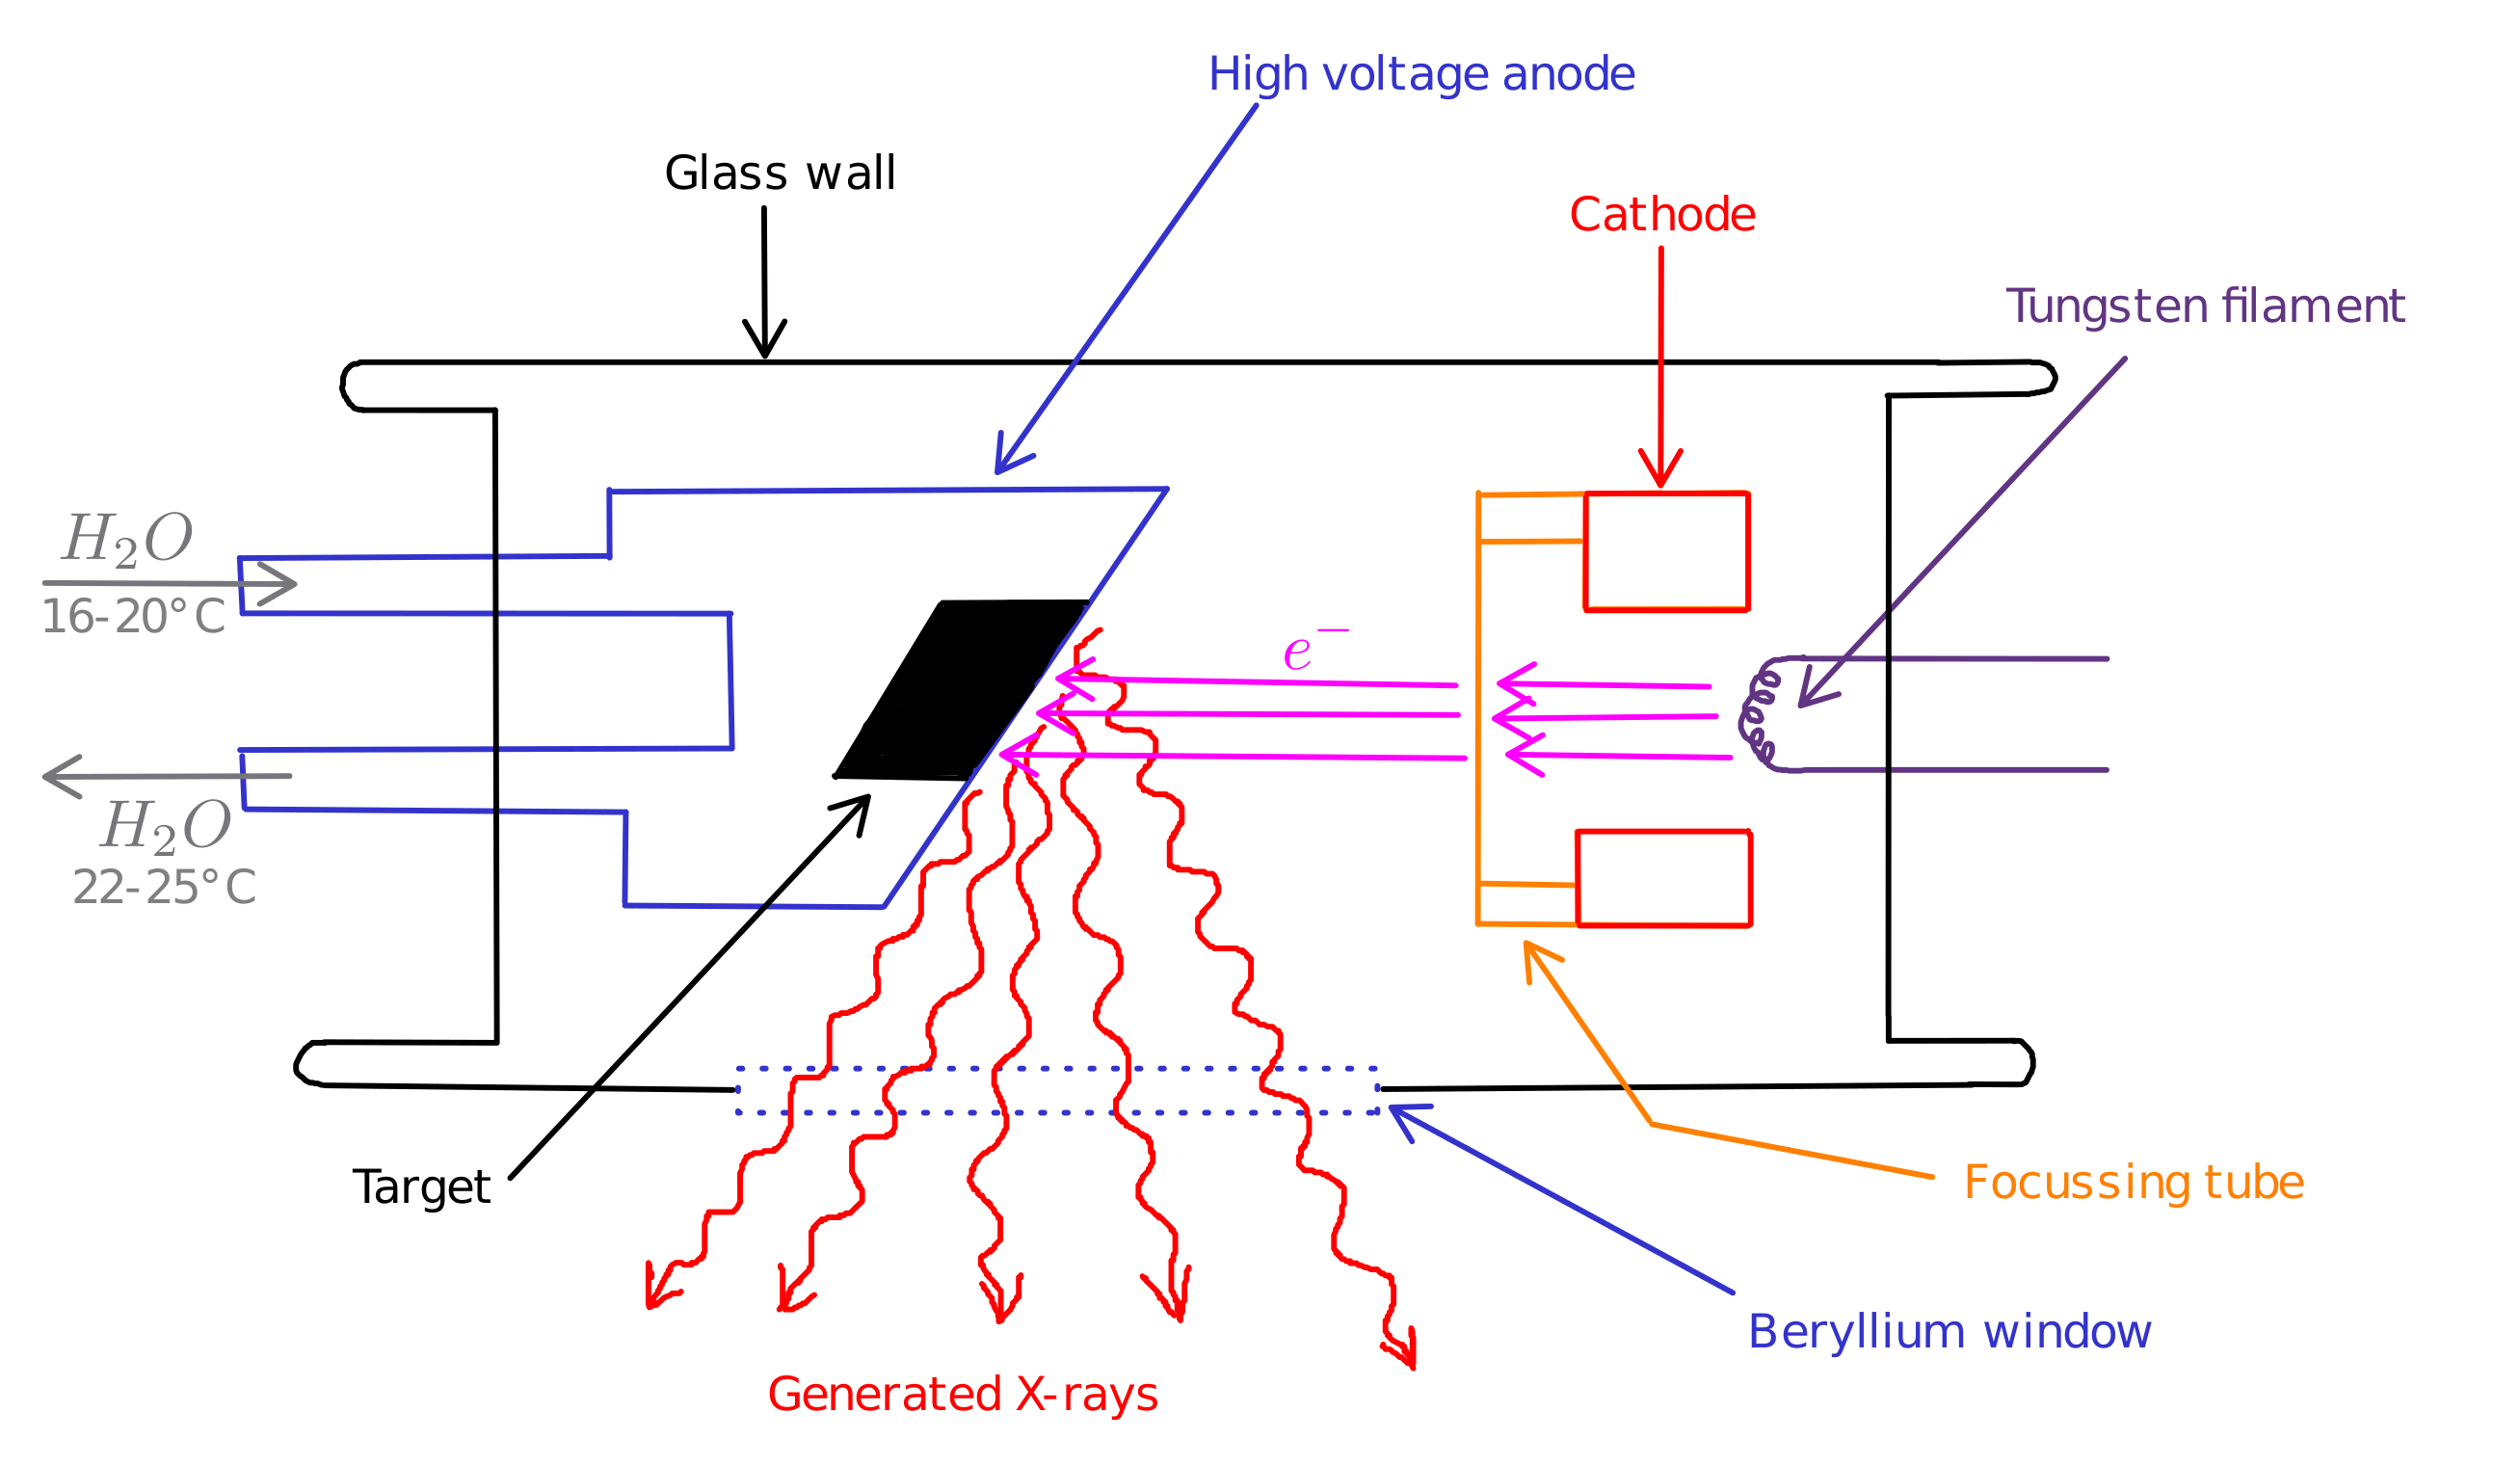
\includegraphics[scale=0.14]{xray_tube.png}
	\caption{\label{fig:xray_tube}Schematic of a X-ray tube.}
\end{figure}

	Figure~\ref{fig:xray_tube} shows the schematic of an X-ray tube. The potential difference between the anode to cathode is around $20-60~\si{kV},$ while the Tungsten filament is supplied a current of $\sim 2-50~\si{mA}.$ The target is composed of the material from which we want to generate the X-rays (generally Cu, Mo or Ag). The Beryllium window provides a transparent region for the generated X-rays to pass through.
	
	The tube is not allowed to cool down between experiments. In the stand-by state, the filament current is reduced to around $\SI{5}{mA}$ and the anode potential is also reduced to $\SI{20}{kV}.$ When data collection is started, the anode voltage is increased to $>\SI{50}{kV}$ and the current in the Tungsten filament is increased to $\SI{40}{mA}.$ In this state, the heated Tungsten filament generates electrons, which are then accelerated and finally hit the target at the anode.

\begin{figure}[h]
	\centering
	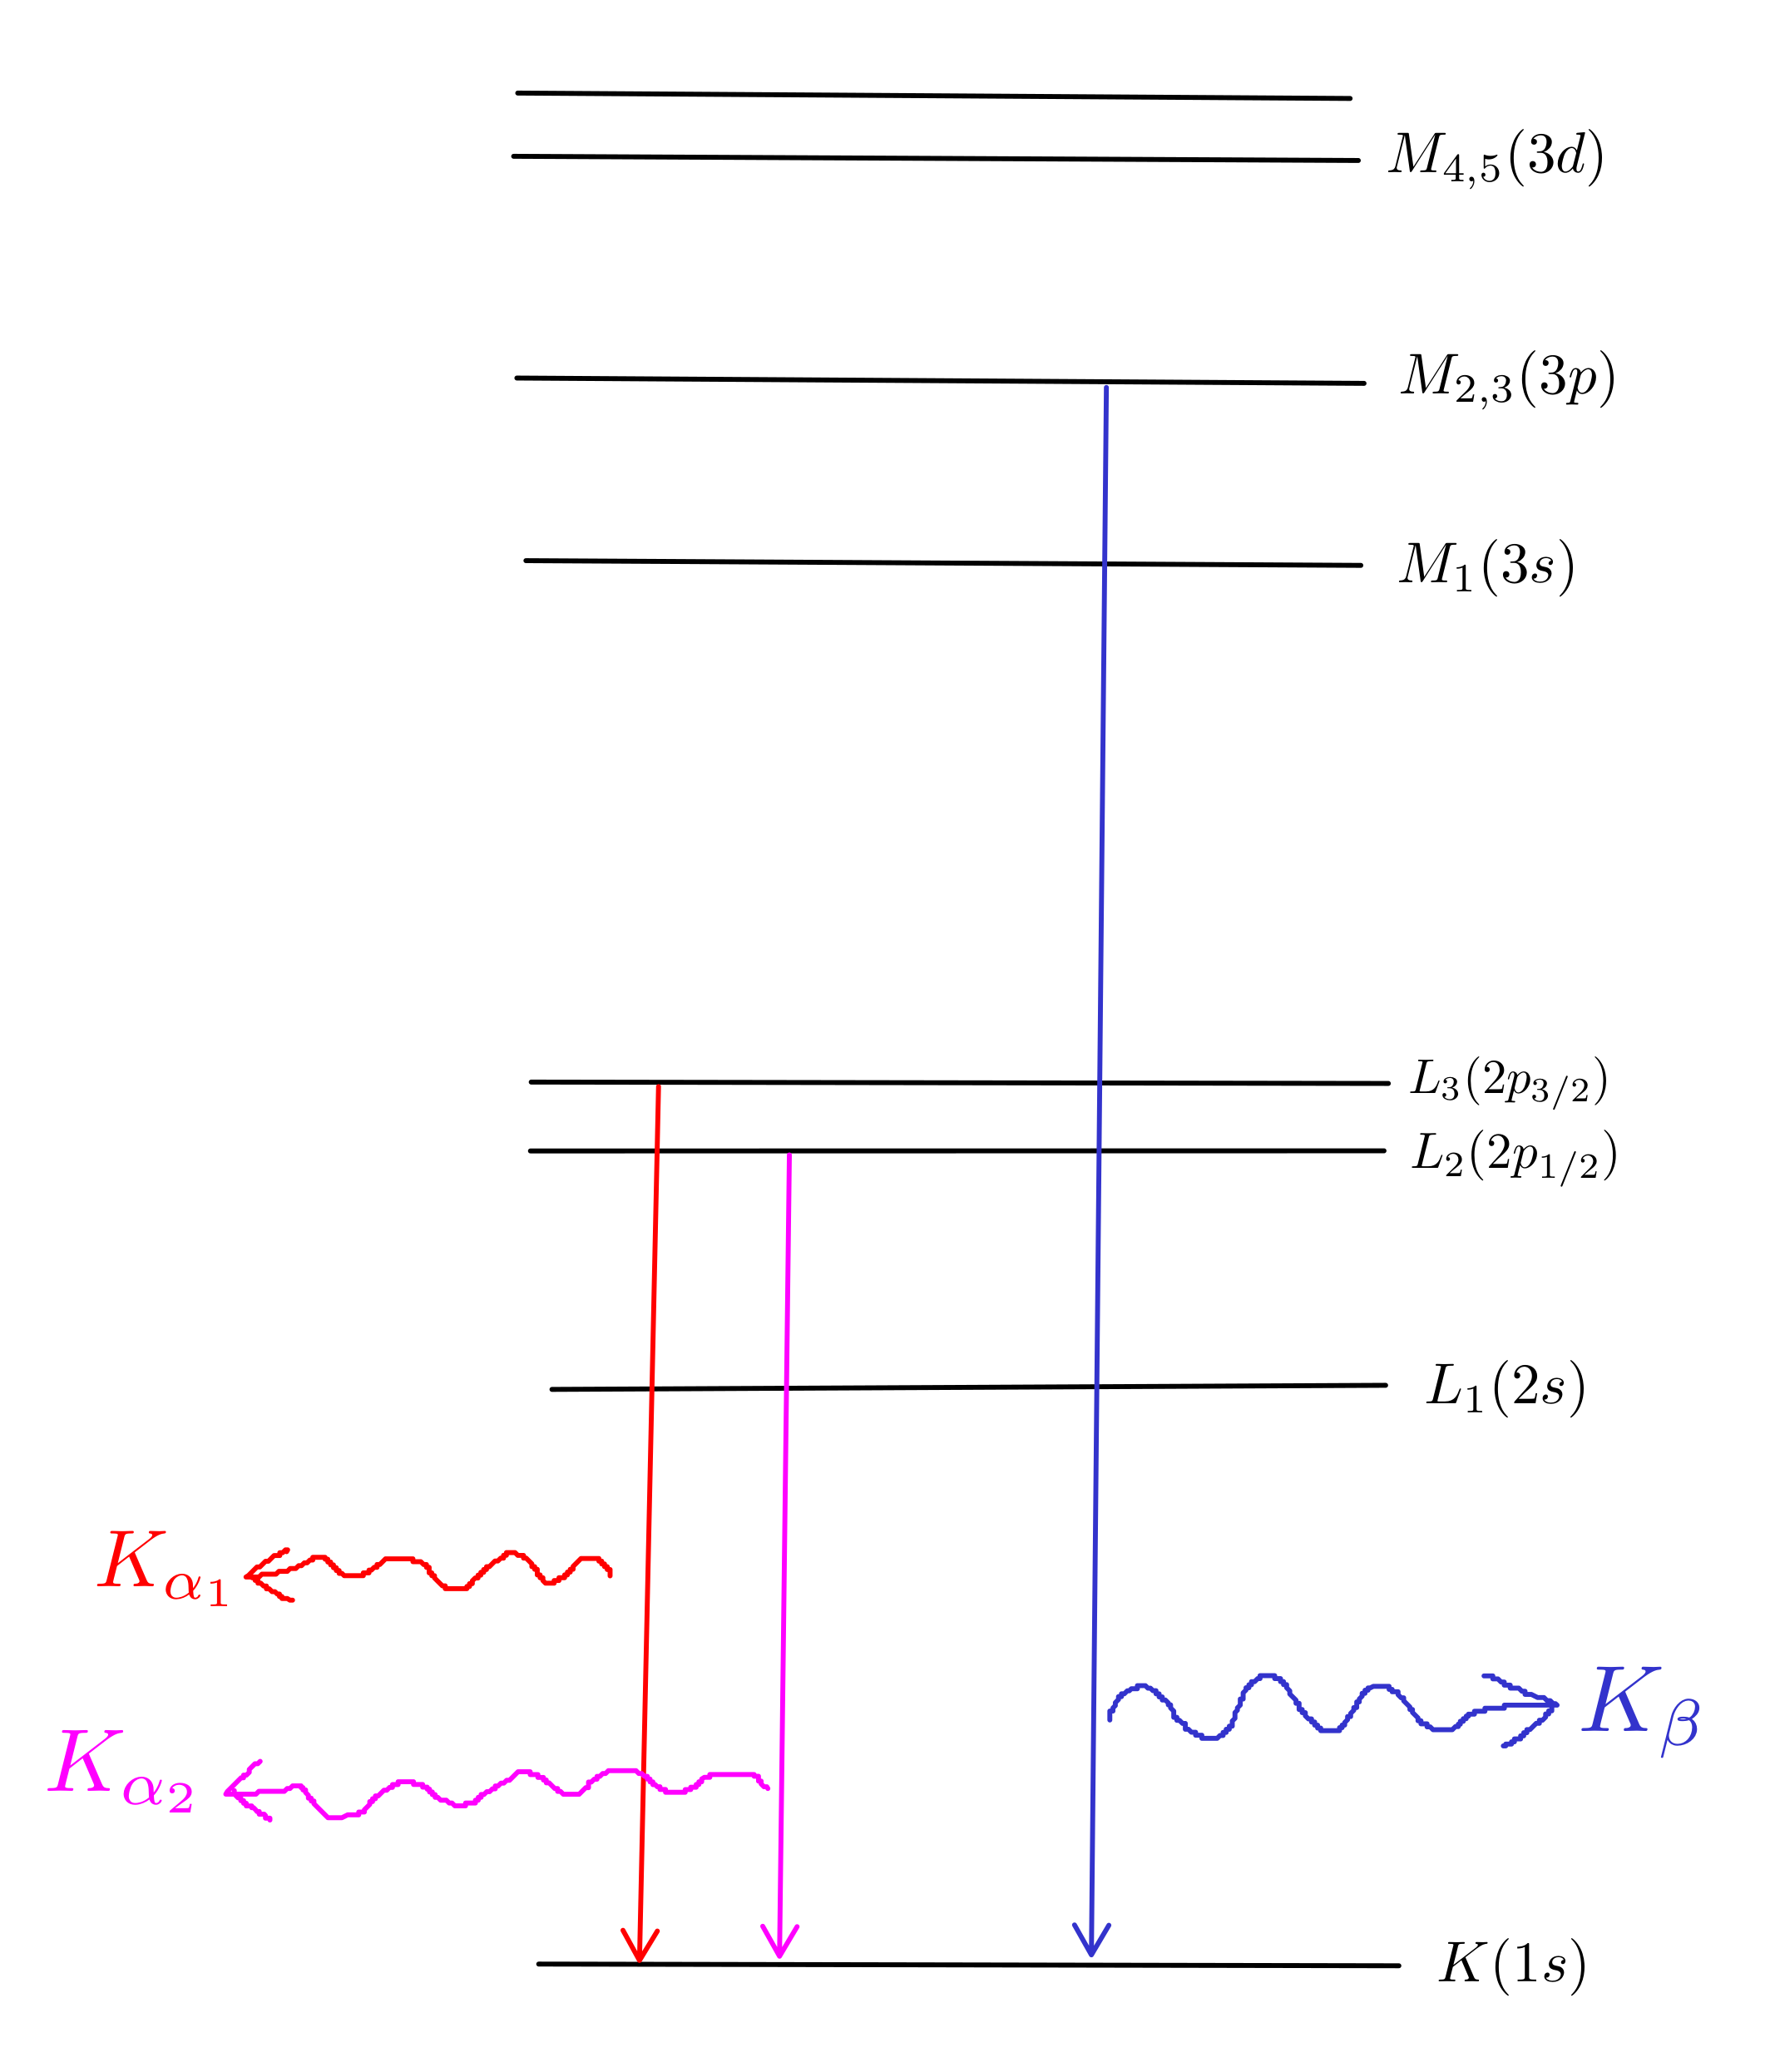
\includegraphics[scale=0.1]{characteristic_xray_transitions.png}
	\caption{\label{fig:xray_transitions}Transitions giving rise to characteristic X-rays.}
\end{figure}
	
	These electrons are able to knock out electrons from the K-shell of an atom in the target. Once an electron is removed from the K-shell, electrons from higher energy levels release energy and come to the K-shell. This release energy is the characteristic X-rays of the material. There are three possible transitions which give rise to X-rays of three different wavelengths. These are shown in figure~\ref{fig:xray_transitions}.
	
\begin{figure}[h]
	\centering
	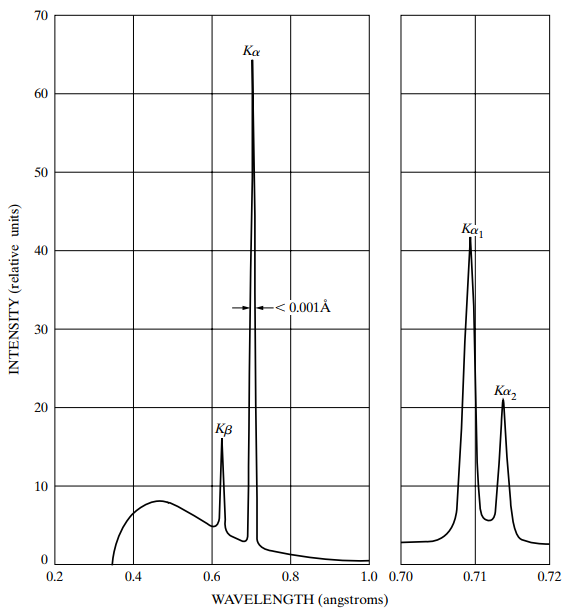
\includegraphics[scale=0.6]{xray_peaks.png}
	\caption{\label{fig:xray_spctra_Cu_Mo}X-ray spectra of $\mathrm{Mo}$ at $\SI{35}{kV}$. The $K_\alpha$ is shown expanded on the right. Picture courtesy:~\cite{Cullity2014}.}
\end{figure}
	
	The X-ray spectra of Mo is shown in figure~\ref{fig:xray_spctra_Cu_Mo}. The $K_\alpha$ peaks are very close to each other. The wavelengths can be found in table~\ref{tab:wavelengths}. The background radiation or white X-rays is attributed to Bremsstrahlung, which is the radiation emitted by electrons when they are decelerated in the X-ray tube.
	
\begin{table}
	\centering
	\caption{\label{tab:wavelengths}Wavelengths of characteristic radiations of Cu and Mo.}
	\begin{tabular}{|c|C|C|C|C|C|c|}
	
		\hline
		
		Source & K_{\alpha_1} (\si{\angstrom}) & K_{\alpha_2} (\si{\angstrom}) & \multicolumn{1}{c|}{\makecell{$K_\alpha$ (average)\\($\si{\angstrom}$)}} & K_\beta (\si{\angstrom}) & Z & $\beta$ filter\\
		
		\hhline{|=|=|=|=|=|=|=|}
		
		Cu & 1.5405 & 1.5433 & 1.5418 & 1.3922 & 29 & Ni (Z = 28) \\
		
		\hline
		
		Mo & 0.7093 & 0.7136 & 0.7107 & 0.6393 & 42 & Nb (Z = 41)\\
		
		\hline
	
	\end{tabular}
\end{table}
	
	We use monochromatic radiation for X-ray diffraction experiments. For this, we have to filter out the unwanted $K_\beta$ and $K_{\alpha2}$ radiations. To filter the $K_\beta$ spectra, we use a $\beta$-filter. The  $\beta$-filters used for Cu and Mo are listed in table~\ref{tab:wavelengths}.
	
	To separate $K_{\alpha1}$ from $K_{\alpha2}$, we use a crystal monochromator. For this, a $\mathrm{Ge}$ crystal is cut along the $(111)$ plane, and the beam with mixed radiation is shined on this plane. Since the two radiations have different wavelengths, they will diffract at two different angles. We can eliminate the unwanted $K_{\alpha2}$ in this way. However, note that \ifnt{the intensity of the reflected beam will fall severely} due to loss of intensity upon reflection.
	
	\section{The physics behind X-ray diffraction}

Max von Laue discovered the phenomena of diffraction of X-rays by crystals, for which he was awarded the Nobel Prize in Physics in 1914. Laue viewed the three-dimensional periodic arrangement of atoms in a crystal as a 3D diffraction grating, and thereby derived a condition which needs to be satisfied for the diffraction of X-rays to take place.

Sir William Henry Bragg and William Lawrence Bragg furthered the physics of X-ray diffraction. Lawrence Bragg, in contrast to Laue's work, viewed the layers (planes) of atoms in the crystal lattice as reflecting surfaces, and X-ray beams reflecting off consecutive planes would interfere constructively if a certain condition was satisfied. This theory is not true in the physical sense -- planes of atoms do not reflect X-rays as such -- but it is correct in the geometrical sense, and we can arrive at Bragg's Law if we start from Laue's condition. The Braggs were jointly awarded the Nobel prize in Physics in 1915 for their work in X-ray crystallography.

\subsection{Bragg's Analysis}
	
	\begin{figure}
	\centering
	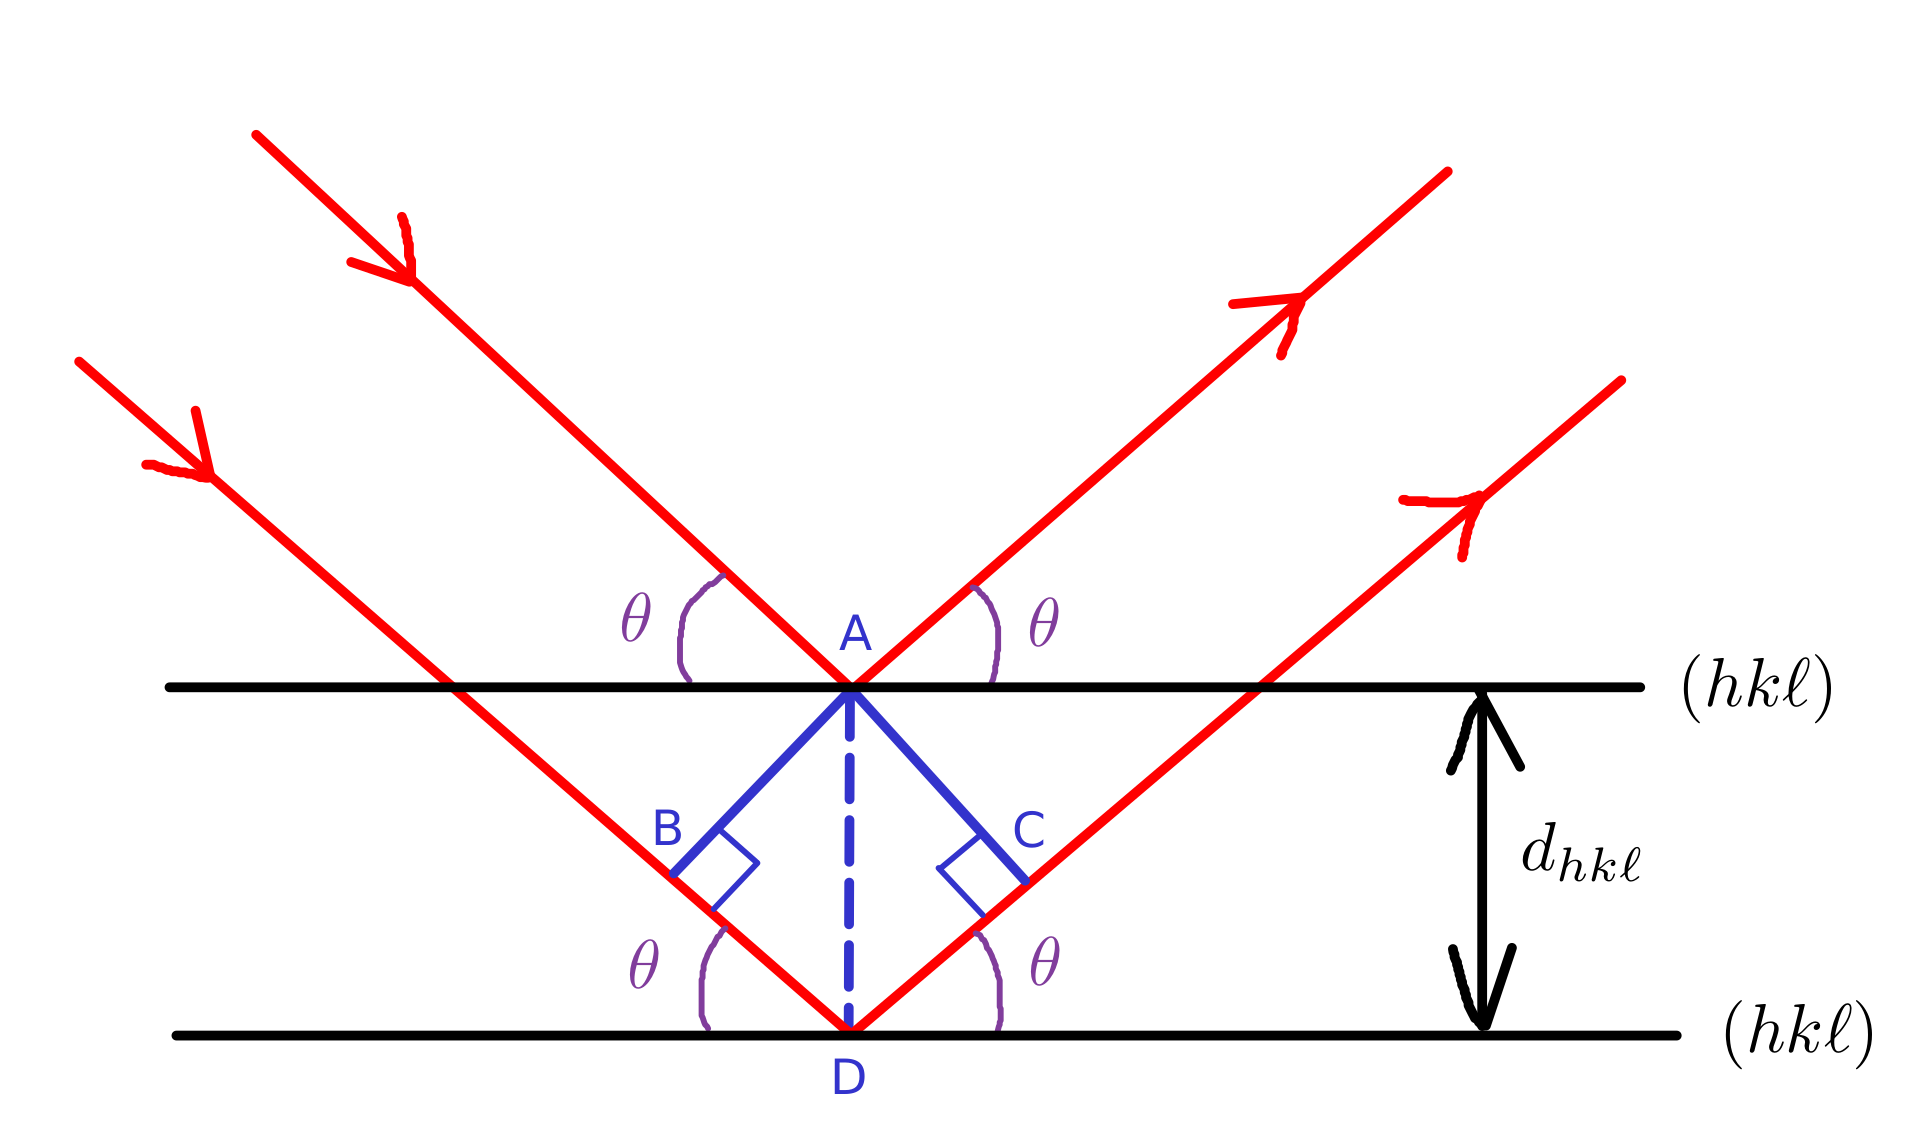
\includegraphics[scale=0.15]{bragg_law.png}
	\caption{\label{fig:bragg_law}X-ray beam is incident on a set of planes with Miller indices $(hk\ell),$ as shown. We draw perpendiculars $\mathrm{AB}$ and $\mathrm{AC}$. $d_{hk\ell}$ is the perpendicular distance between two planes with the same Miller indices $(hk\ell).$}
	\end{figure}

	Derivation of Bragg's Law is straightforward. Referring to figure~\ref{fig:bragg_law}, the path difference,%
%	
	\begin{align}
	\mathrm{P.D.} &= \mathrm{BD} + \mathrm{DC} \nonumber\\
				&= 2 d_{hk\ell} \sin \theta.
	\end{align}
	
	For constructive interference,%
%	
	\begin{align}
	&\phantom{\implies} \mathrm{P.D.} = n \lambda,\quad n \in \mathbb{Z} \nonumber\\
	&\implies \boxed{2 d_{hk\ell} \sin \theta = n \lambda}
	\end{align}
%	
	which is Bragg's Law for X-ray diffraction. $n$ is the order of diffraction or reflection.
	
%***************************************************************************************************
	
\subsection{Laue's analysis}

	\begin{figure}
	\centering
	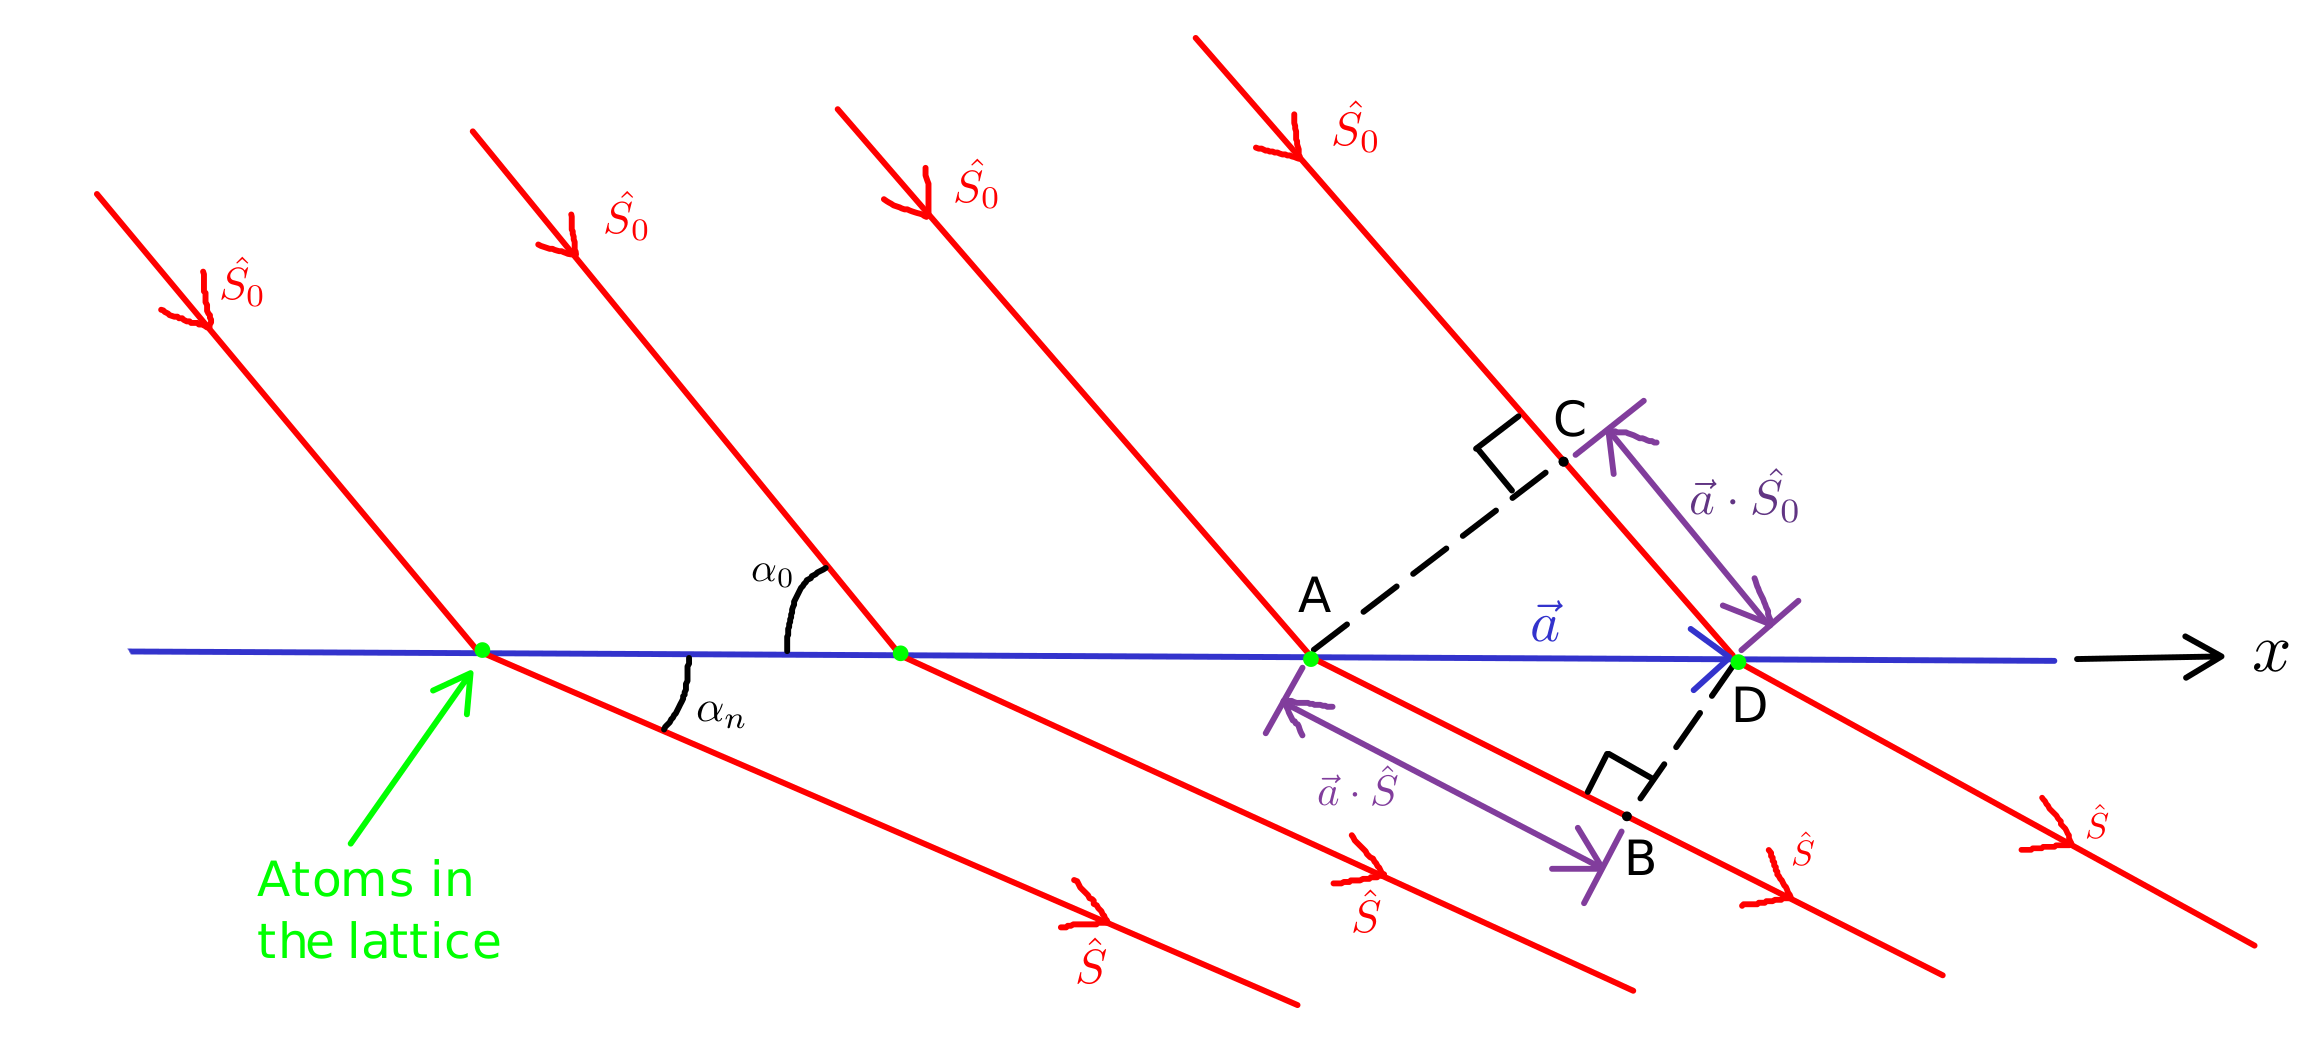
\includegraphics[scale=0.17]{laue_analysis.png}
	\caption{\label{fig:laue_analysis}Diffraction from a lattice row along the $x$ axis. The incident and diffracted beams make angles $\alpha_0$ and $\alpha_n$ respectively with the lattice row. $\vec{a}$ is the lattice translation vector. Adapted from \cite{Hammond2015}.}
	\end{figure}
	
	Consider a simple crystal with one atom as the basis, as shown in figure~\ref{fig:laue_analysis}. The atoms are regarded as the scattering centres from which the diffraction takes place. $\hat{S_0}$ and $\hat{S}$ are two unit vectors in the direction of the incident and diffracted beam, respectively. The lattice spacing is $a$.
	
	The path difference,%
%		
		\begin{align}
		\mathrm{P.D.} &= \mathrm{AB - CD}, \nonumber\\
					  &= a \qty( \cos \alpha_n - \cos \alpha_0 ) \\
					  &= \va{a} \cdot \qty( \vu{S} - \vu{S_0} ),
		\end{align}%
%		
	has to be an integer multiple of wavelength for constructive interference.%
%		
		\begin{equation}
		\therefore \boxed{a \qty( \cos \alpha_n - \cos \alpha_0 ) = \va{a} \cdot \qty( \vu{S} - \vu{S_0} ) = n_x \lambda,} \quad n_x \in \mathbb{Z}. \label{eq:1st_laue_eqn}
		\end{equation}
		
	Eqn.~\eqref{eq:1st_laue_eqn} is the \textbf{first Laue equation}.
	
	This path difference is still valid if the diffracted beam, instead of being below the row of atoms, is above it, or is out of the plane of the paper itself. Therefore, all diffracted beams with the same path difference occur at the same angle to the atom row. Thus, all diffracted beams lie on the surface of a cone, known as the \bfnt{Laue cone}, centred on the atom row with semi-apex angle $\alpha_n.$ This is illustrated in figure~\ref{fig:laue_cones}.
	
	\begin{figure}
	\centering
	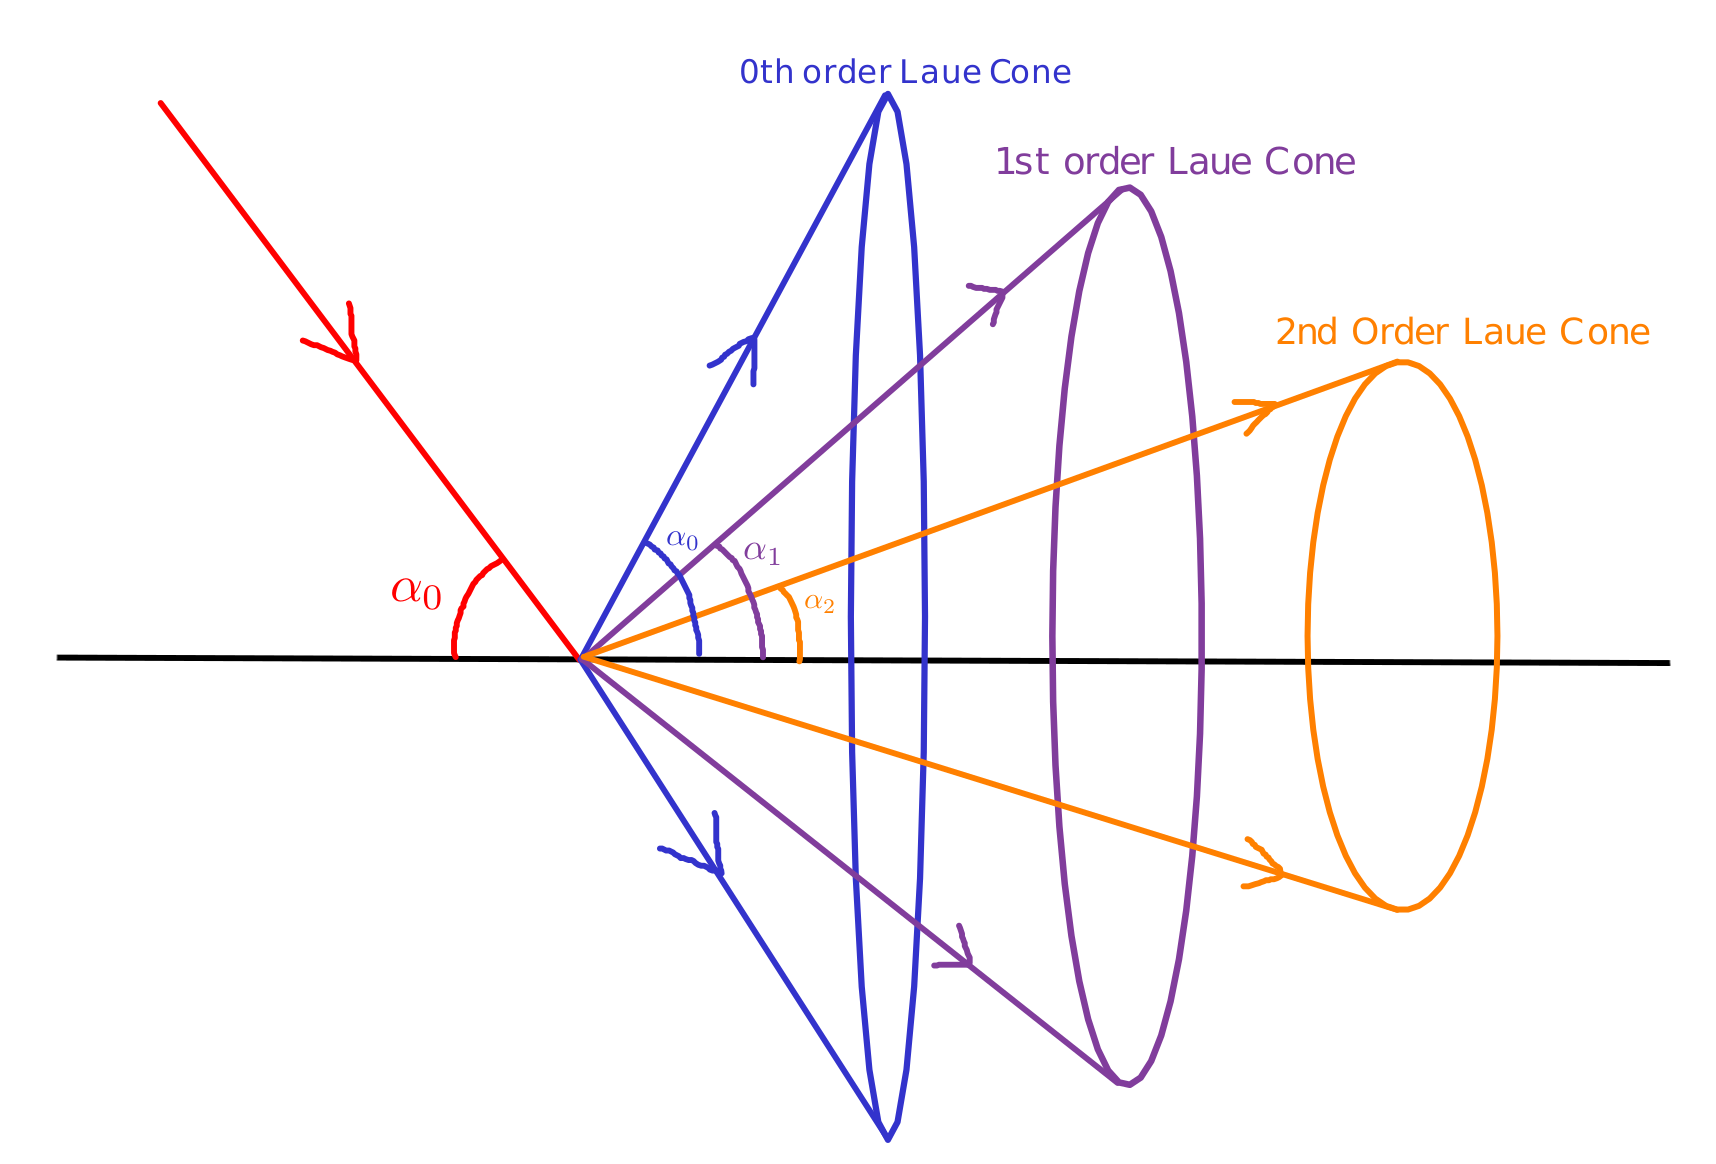
\includegraphics[scale=0.17]{laue_cones.png}
	\caption{\label{fig:laue_cones}Three Laue cones representing the direction of diffracted beam from a lattice row along the $x$-axis, with $0$ ($n_x = 0$), $\lambda$ ($n_x = 1$) and $2\lambda$ ($n_x = 2$) path differences. Similar cones also lie to the left of the 0th order cone for $n < 0.$}
	\end{figure}
	
	Proceeding similarly, we can derive two more equations for diffraction from atom rows along the $y$ and $z$ directions, thereby arriving at the second and third Laue equations:%
%		
	\begin{align}
	\boxed{b \qty( \cos \beta_n - \cos \beta_0 ) = \va{b} \cdot \qty( \vu{S} - \vu{S_0} ) = n_y \lambda,} \quad n_y \in \mathbb{Z}; \label{eq:2nd_laue_eqn} \\[1.5em]
	\boxed{c \qty( \cos \gamma_n - \cos \gamma_0 ) = \va{c} \cdot \qty( \vu{S} - \vu{S_0} ) = n_z \lambda,} \quad n_z \in \mathbb{Z}. \label{eq:3rd_laue_eqn}
	\end{align}
	
	For constructive interference to simultaneously occur from all the three atom rows in the three directions, all three Laue equations must be satisfied simultaneously. This is geometrically equivalent to three Laue cones intersecting at some points. Diffraction will only occur along those directions in which three Laue cones intersect.
	
%***********************************************************************************************


\subsection{The reciprocal lattice}

	\begin{figure}
	\centering
	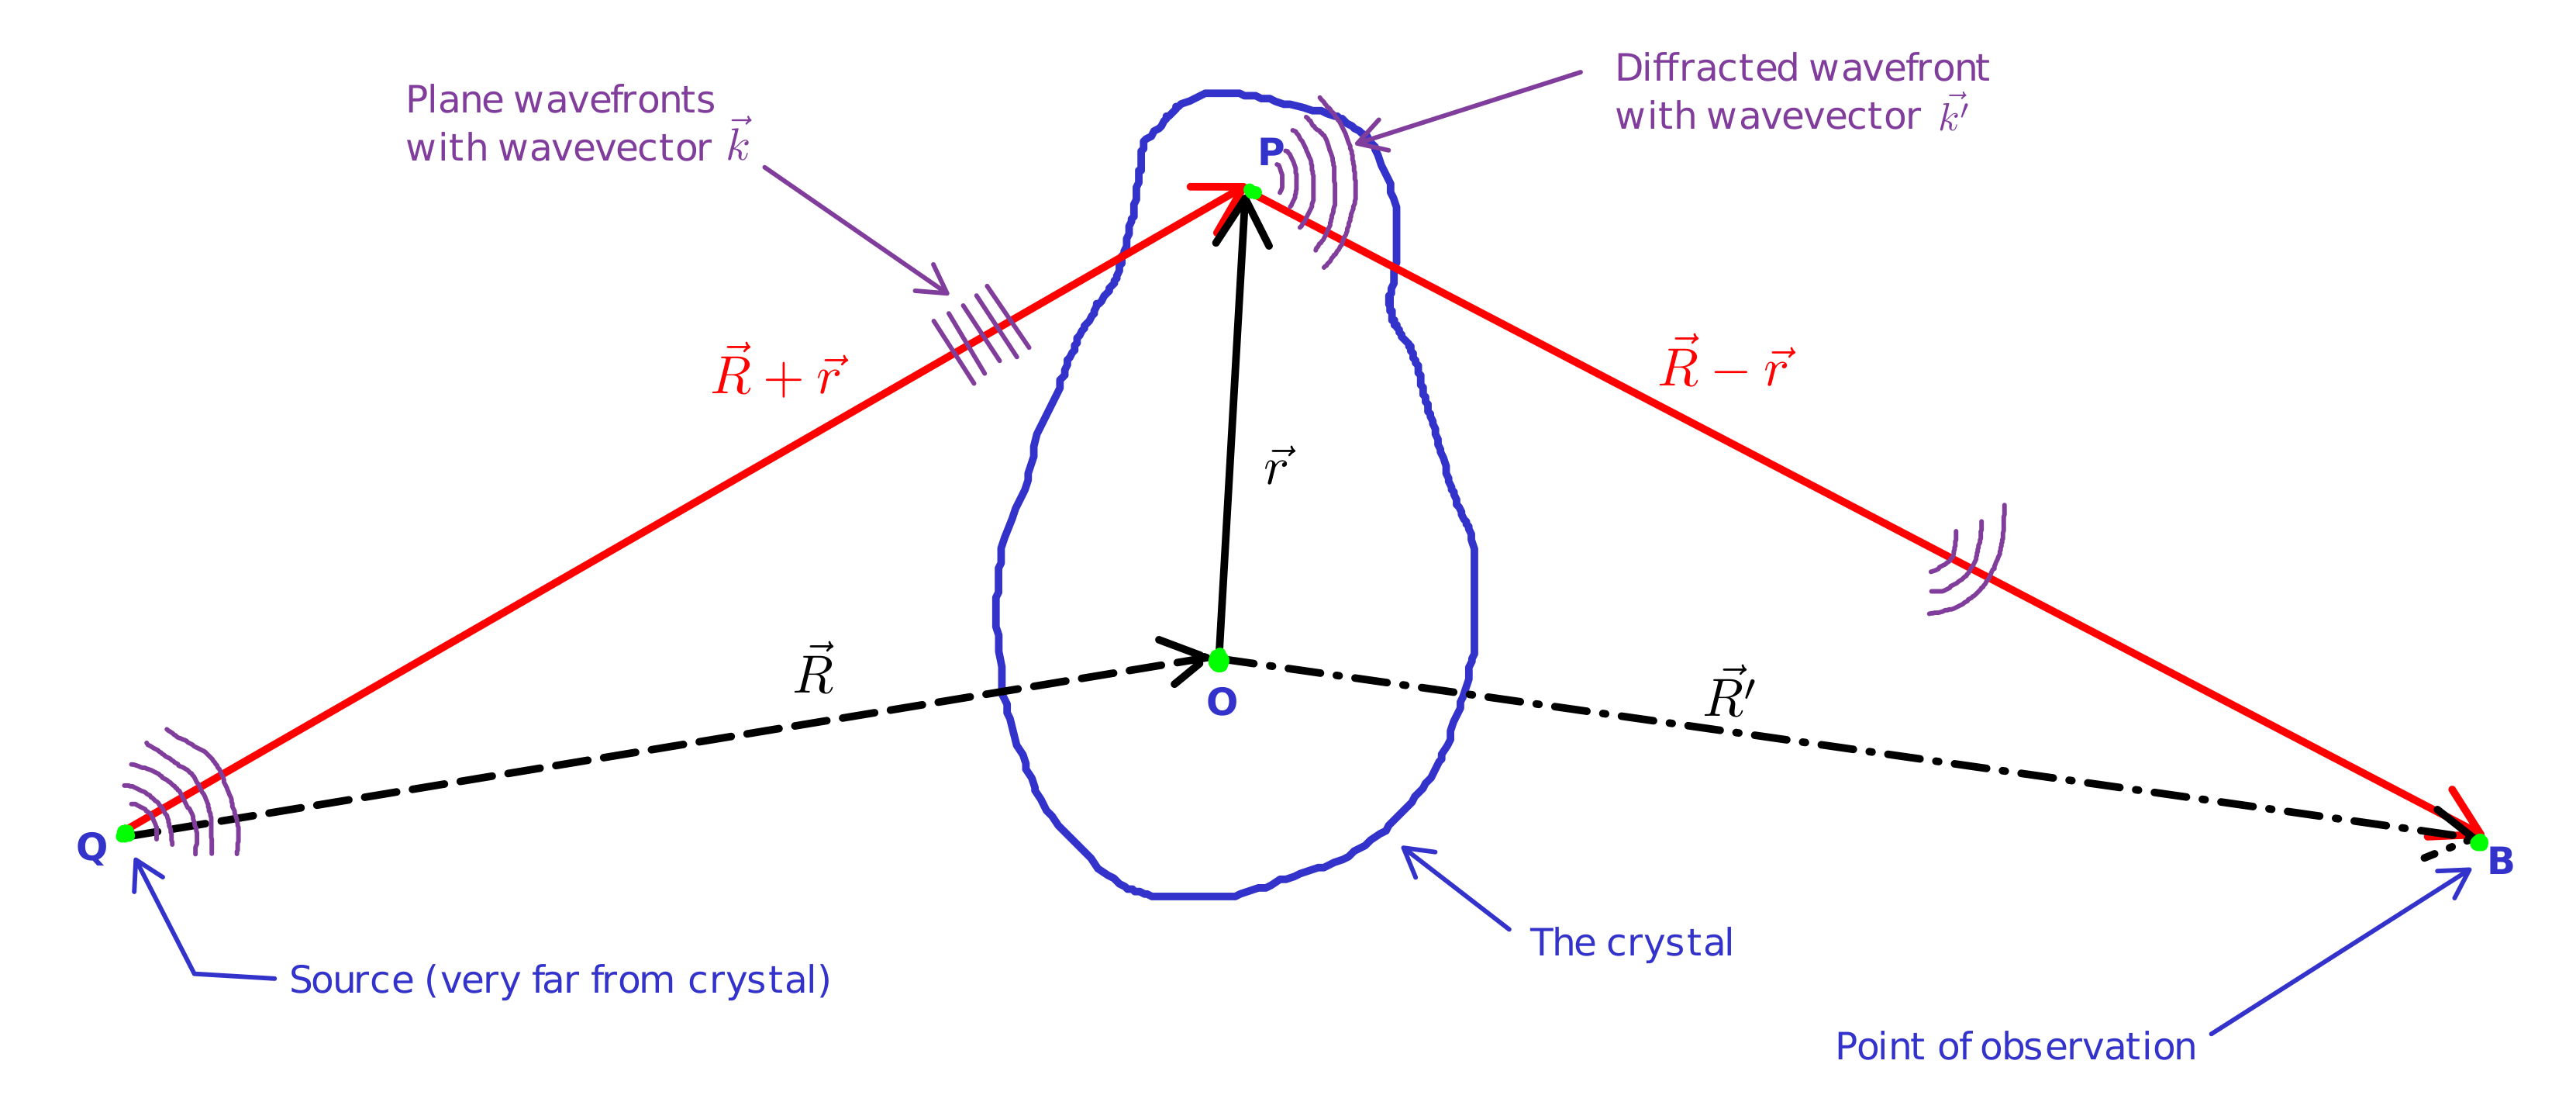
\includegraphics[width=\textwidth]{reciprocal_lattice.png}
	\caption{\label{fig:reciprocal_lattice}A plane wavefront with wavevector $\va{k}$ reaches a crystal, and is diffracted by an atom at point $P.$ We observe the diffracted beam, with wavevector $\va{k'}$, from point $B.$ Figure adapted from \cite{Harbola2021}.}
	\end{figure}

	Consider the situation shown in figure~\ref{fig:reciprocal_lattice}. The source of X-rays is very far away from the crystal; hence, the wavefront reaching the crystal can be considered to be a plane wavefront. We observe from point $B.$
	
	The plane wave reaches the point $P$ with an amplitude%
%		
		\begin{equation}
		A_P = A_0 ~ \e{i \va{k} \vdot \qty( \va{R} + \va{r} )} ~ \e{-i \omega_0 t}
		\end{equation}

	The amplitude of the waves reaching $B$ will depend on $A_P$ and density of scatterers at $P.$ The spherical waves generated from $P$ and reaching point $B$ will have the form%
%		
		\begin{equation}
		A_B = A_P ~ \rho(\va{r}) ~ \dfrac{\e{i \va{k'} \vdot ( \va{R'} - \va{r} ) }}{\abs{ \va{R'} - \va{r} }},
		\end{equation}%
%		
	where $\rho(\va{r})$ is the density of scatterers at $P.$ We assume that these scatterers are all in phase, and act as secondary sources.\\
	
	Assume $\va{R'} \gg \va{r}.$\\[0.8em]
	$\implies \abs{ \va{R'} - \va{r} } \approx \abs{\va{R'}} = R'$
	
	\begin{align}
	\therefore A_B &= \dfrac{A_0 \rho(\va{r})}{R'} ~ \e{i \va{k} \vdot ( \va{R} + \va{r} )} ~ \e{ i \va{k}' \vdot (  \va{R}' - \va{r}) } \nonumber \\[0.8em]
		&= \underbrace{\dfrac{A_0 \rho(\va{r})}{R'} ~ \e{ i ( \va{k} \vdot \va{R} + \va{k}' \vdot \va{R}' ) }}_{\text{constant}} ~ \e{i ( \va{k} - \va{k'} ) \vdot \va{r}}.
	\end{align}
	
	Let%
%		
		\begin{equation}
		\va{\kappa} = \va{k}' - \va{k}
		\end{equation}%
%		
	be the \textbf{scattering vector}.
	
	The net intensity due to all such points $P$ in the crystal is given by%
%		
		\begin{align}
		I &\propto \abs{ \int_V A_B(\va{r}) \dd[3]{r} }^2 \nonumber \\[1em]
		  &\propto \dfrac{A_0^2}{R'^2} \abs{ \int_V \dd[3]{r} \rho(\va{r}) ~ \e{ - i \va{\kappa} \vdot \va{r} } }  ^2. \label{eq:net_I}
		\end{align}
		
	$\va{R}$ is the lattice translation vector, defined by%
%		
	\begin{equation}
	\va{R} = \sum_{i=1}^3 n_i \va{a}_i
	\end{equation}%
%	
	where $\va{a}_i$ are the basis vectors, and $n_i \in \mathbb{Z} ~ \forall ~ i.$
	
	Expanding $\rho(\va{r})$ in terms of Fourier components,%
%		
	\begin{equation}
	\rho(\va{r}) = \sum_{\va{G}} \rho_{\va{G}} ~ \e{ i \va{G} \vdot \va{r} } \label{eq:fourier_rho}
	\end{equation}
%	
	and%
%	
	\begin{equation}
	\rho(\va{r} + \va{R}) = \sum_{\va{G}} \rho_{\va{G}} ~ \e{ i \va{G} \vdot \va{r} } ~ \e{ i \va{G} \vdot \va{R} }.
	\end{equation}
	
	Due to translational invariance in a Bravais lattice,%
%	
	\begin{align}
	&\phantom{\implies} \rho (\va{r}) = \rho( \va{r} + \va{R} ) \nonumber \\
	&\implies \boxed{ \e{i \va{G} \vdot \va{R} } = 1.} \\ \label{eq:reci_lattice_cond}
	&\implies \va{G} \vdot \va{R} = 2\pi m, \quad m \in \mathbb{Z}.
	\end{align}
	
	This $\va{G}$ is the translation vector of the reciprocal lattice. Given any lattice in real space, we can generate a lattice in reciprocal space keeping in mind equation~\eqref{eq:reci_lattice_cond}.
	
	If%
%	
	\begin{equation}
	\va{G} = h \va{g}_1 + k \va{g}_2 + \ell \va{g}_3,\label{eq:reci_lattice_vec}
	\end{equation}%
%	
	then we have%
%	
	\begin{equation}
	\va{g}_i \vdot \va{a}_j = 2\pi \delta_{ij}.\label{eq:relation_g_a}
	\end{equation}%
	
	One expression that satisfies this condition is%
%	
	\begin{equation}
	\va{g}_1 = 2\pi \dfrac{\va{a}_2 \cross \va{a}_3}{\qty[ \va{a}_1 ~ \va{a}_2 ~ \va{a}_3 ]}
	\end{equation}%
%	
	and so on.
	
	Returning to Eqn.~\eqref{eq:net_I}, substituting eqn.~\eqref{eq:fourier_rho}, we have%
%	
	\begin{align}
	I &\propto \dfrac{A_0^2}{R'^2} \abs{ \sum_{\va{G}} \int_V \dd[3]{r} \rho_{\va{G}} ~ \e{ i (\va{G} - \va{\kappa}) \vdot \va{r} } }  ^2 \nonumber \\[1em]
	  &\propto \dfrac{A_0^2}{R'^2} \abs{ \sum_{\va{G}} \rho_{\va{G}} \int_V \dd[3]{r} \e{ i (\va{G} - \va{\kappa}) \vdot \va{r} } }^2
	\end{align}%
	
	If $\va{G} = \va{\kappa},$ the above integral evaluates to $V.$ If $\va{G} \ne \va{\kappa},$ the integral is $0$ as it an integration of sines and cosines over the entire volume. Thus,%
%	
	\begin{equation}
	\int_V \dd[3]{r} \e{ i (\va{G} - \va{\kappa}) \vdot \va{r} } = \delta ( \va{G} - \va{\kappa} ) \cdot V.
	\end{equation}
	
	Therefore, the condition under which $I \ne 0$ is%
%	
	\begin{equation}
	\boxed{\va{\kappa} = \va{G}}
	\end{equation}%
%	
	i.e. when the reciprocal space lattice translation vector = scattering vector. This is known as \bfnt{Laue's condition} for X-ray diffraction.
	
	As a parting note, it should be mentioned that the vector $\va{G}_{hk\ell},$ written as in eqn.~\eqref{eq:reci_lattice_vec}, is perpendicular to the plane whose Miller indices are given by $(h k \ell).$
		
%--------------------------------------------------------------------------------------------------

\subsection{Ewald's Sphere}
	
	\begin{figure}
	\centering
	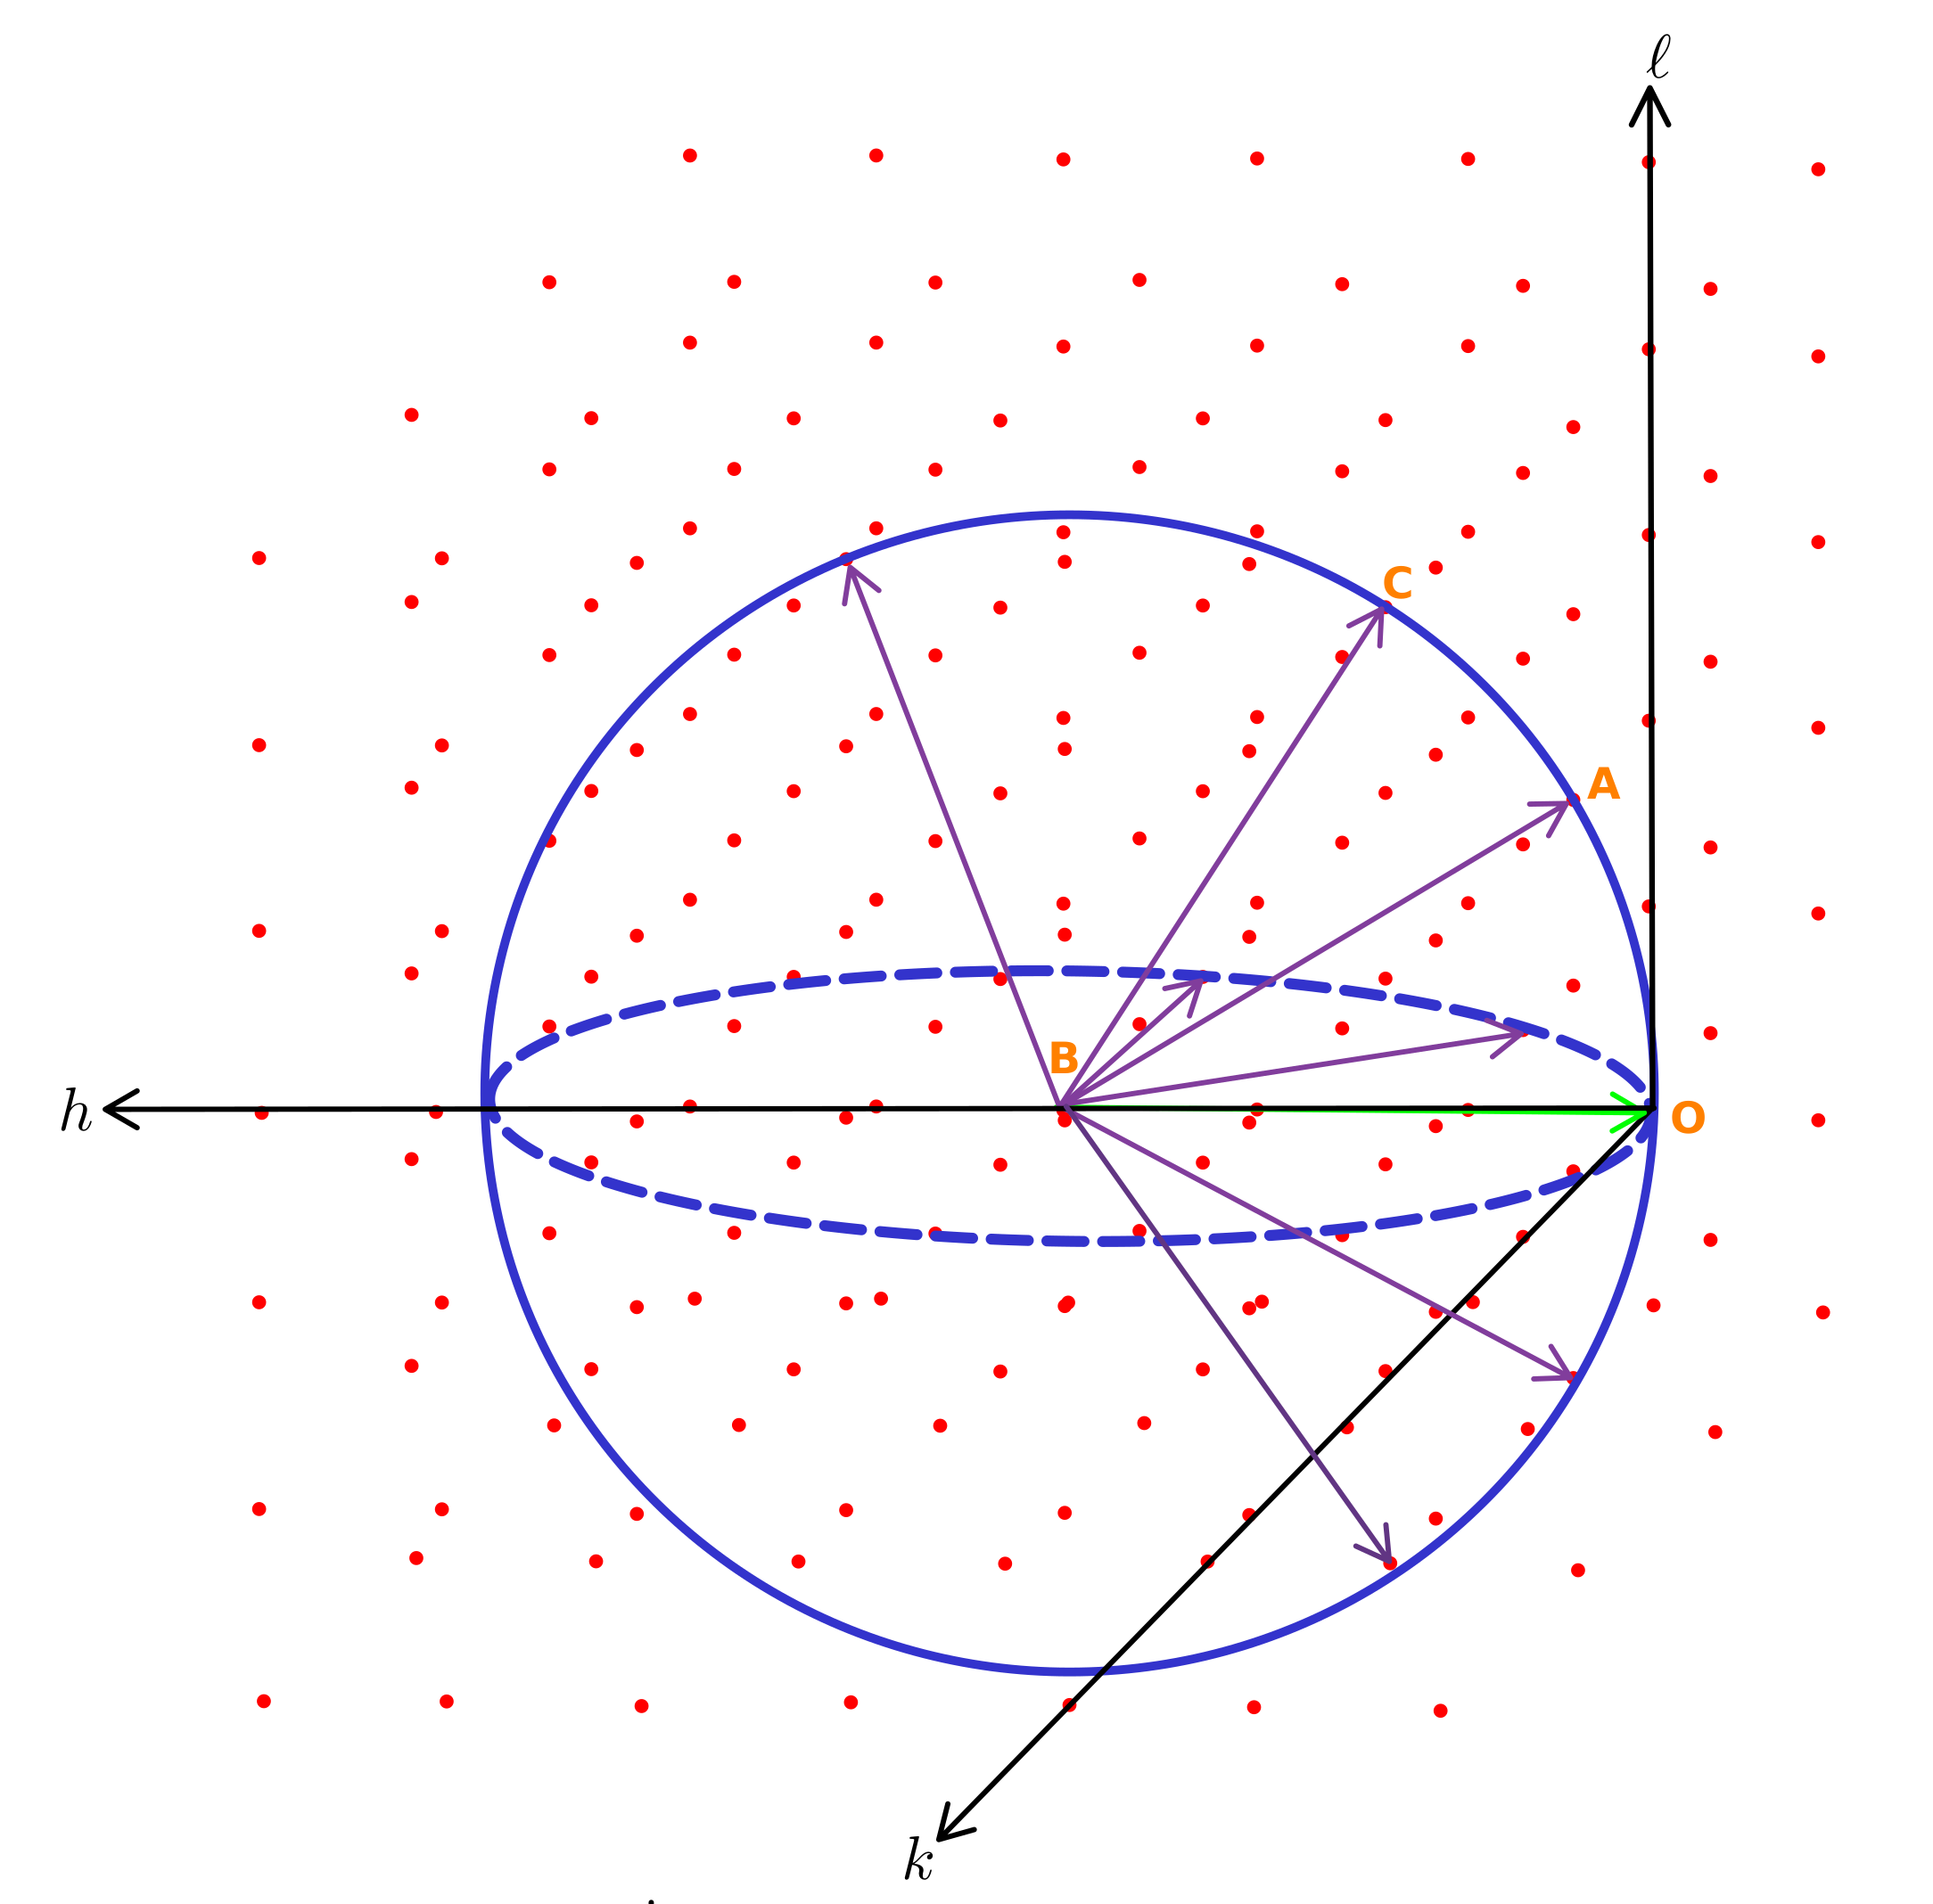
\includegraphics[scale=0.15]{ewald_sphere.png}
	\caption{\label{fig:ewald_sphere}Ewald's sphere construction in three dimensional reciprocal space. Each point in the reciprocal space corresponds to a set of planes in the real space with Miller indices same as that of the coordinates of the point. The green line is the wave vector of the incident X-ray beam, with $\overrightarrow{BO} \equiv \va{k}.$ We draw the sphere with the origin at the tail of the incident wave vector, $B,$ and with a radius~$= \abs*{\va{k}} = 2\pi / \lambda.$ The blue sphere thus drawn is Ewald's sphere. All the purple arrows are vectors which end on points on the surface of the sphere. These points satisfy Bragg's Law; therefore, the purple arrows are actually the wave vectors of the X-ray beam diffracted from that particular set of planes.}
	\end{figure}
	
	Refer to figure~\ref{fig:ewald_sphere}. In 3D reciprocal space, each point $(h, k, \ell)$ denotes a particular plane in real space with Miller indices $(hk\ell).$ The vector $\overrightarrow{BO} \equiv \va{k}$ is the wave vector of the incident X-ray beam. A sphere is drawn with the tail of the incident wave vector (point $B$) as the origin, and with a radius~$= \abs*{\va{k}} = \frac{2\pi}{\lambda}.$ This sphere, shown in blue, is Ewald's sphere or the reflecting sphere. Note that the tip of the arrow is taken as the origin of the coordinate system.
	
	In elastic scattering, the wave vector of the diffracted beam will have the same length as that of the incident wave vector, i.e. $\abs*{\va{k}'} = \abs*{\va{k}}.$  Therefore, \textcolor{red}{any point on the surface of the sphere will denote a set of planes that satisfy Bragg's Law}.
	
	Consider the point $A(h_1, k_1, \ell_1).$ It lies on the surface of the sphere, and hence, the set of planes with Miller indices $(h_1 k_1 \ell_1)$ will satisfy Bragg's Law. $\overrightarrow{BA}$ will be the wave vector of the diffracted beam, and $\angle ABO = 2\theta,$ where $\theta$ is the Bragg angle for this particular set of planes. The scattered wave vector $\va{\kappa}$ will be, in this case, $\overrightarrow{AO},$ and, due to Laue's condition, this is the same as the reciprocal lattice vector $\va{G}.$ Thus, we may visualize the incident beam hitting the crystal planes at the point $B,$ and the planes are oriented such that $AO$ is perpendicular to them.
	
	Ewald's sphere, thus, helps us to geometrically understand Laue's condition and the unification of Bragg's Law and Laue's condition.
	
%******************************************************************************************************

\subsection{Structure Factor, Friedel's Law and Centrosymmetry in X-ray Diffraction}

	The atomic scattering factor is given by%
%	
	\begin{equation}
	f = \dfrac{\text{Amplitude scattered by atom}}{\text{Amplitude scattered by single electron}}.
	\end{equation}
	
	At zero scattering angle, all the scattered waves are in phase and the scattered amplitude is the simple sum of the contribution from all $Z$ electrons, i.e. $f = Z$. As the scattering angle increases, $f$ falls below $Z$ because of the increasingly destructive interference effects between the $Z$ scattered waves.

	The scattering amplitude of a unit cell is determined by summing $f$ from all the atoms in a unit cell to all the atoms in a basis. The summation must take into account the path or phase differences between the scattered wave, and is given by the dimensionless structure factor:%
%	
	\begin{equation}
	F_{hk\ell} = \dfrac{\text{amplitude scattered by the atoms in the unit cell}}{\text{amplitude scattered by a single electron}}.
	\end{equation}
	
	$F_{hk\ell}$ must include the phase angle of the scattered wave, and hence, it is a complex number.
	
	\begin{figure}
	\centering
	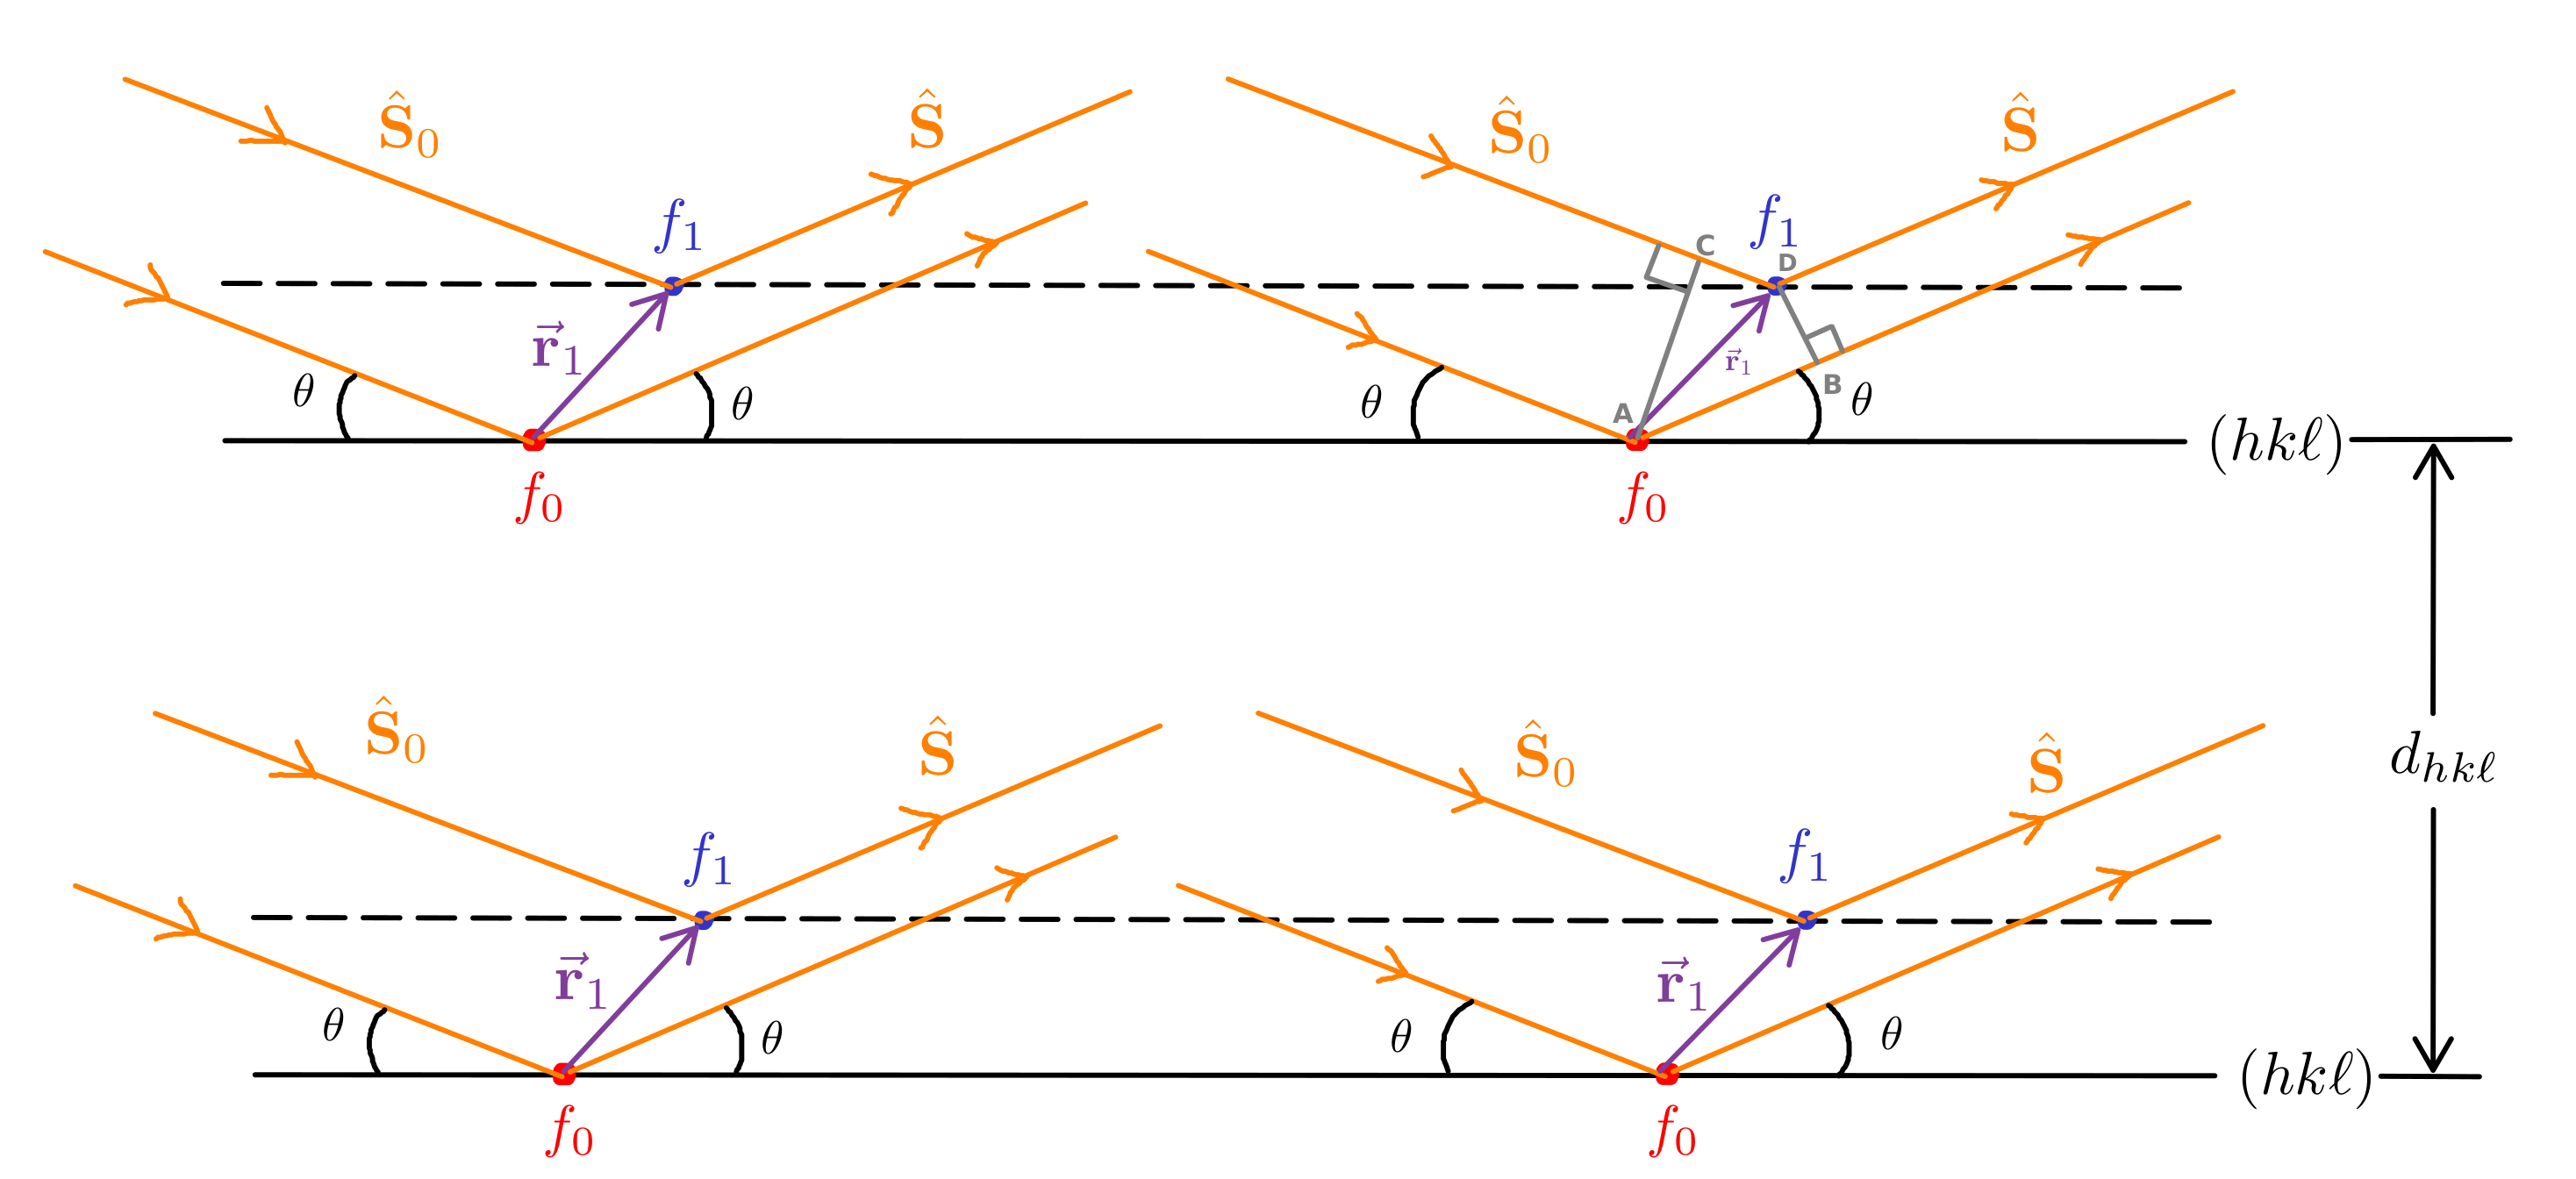
\includegraphics[scale=0.15]{structure_factor.png}
	\caption{\label{fig:struct_fact}Consider a basis with two atoms, one with atomic scattering factor $f_0$, and another with $f_1.$ $\va{r}_1$ is the position vector of one atom w.r.t. the other. $\vu{S}_0$ is a unit vector in the direction of the incoming X-ray beam, while $\vu{S}$ is the unit vector in the direction of the diffracted beam.}
	\end{figure}
	
	Refer to figure~\ref{fig:struct_fact}. The position vector $\va{r}_1$ is written as%
%	
	\begin{equation}
	\va{r}_1 = \sum_{i=1}^3 x_i \va{a}_i
	\end{equation}%
%	
	where $\va{a}_i$ are the lattice basis vectors, and $x_i$ are \textit{fractions} of the cell edge lengths.
	
	The path difference,%
%	
	\begin{align}
	\mathrm{P.D.} &= \mathrm{AB} - \mathrm{CD} \nonumber \\
				  &= \va{r}_1 \vdot \vu{S} - \va{r}_1 \vdot \vu{S}_0 \nonumber \\
				  &= \va{r}_1 \vdot ( \vu{S} - \vu{S}_0 ).
	\end{align}
	
	$\because$ Bragg's Law is satisfied, we can write using eqn.~XXX,%
%		
	\begin{align}
	&\phantom{\implies} ( \vu{S} - \vu{S}_0 ) = \lambda \va{G}_{hk\ell} \nonumber\\
	&\phantom{ \implies ( \vu{S} - \vu{S}_0 ) } = \lambda \qty( h \va{g}_1 + k \va{g}_2 + \ell \va{g}_3 ).\\
	&\implies \mathrm{P.D.} = \lambda \qty( x_1 \va{a}_1 + x_2 \va{a}_2 + x_3 \va{a}_3 ) \vdot \qty( h \va{g}_1 + k \va{g}_2 + \ell \va{g}_3 ) \nonumber \\
	&\implies \mathrm{P.D.} = \lambda \qty( h x_1 + k x_2 + \ell x_3 ).
	\end{align}%
%	
	where we have used $\va{g}_i \vdot \va{a}_j = \delta_{ij}$ to arrive at the last step.
	
	The phase angle is given by%
%	
	\begin{align}
	\phi &= \dfrac{2\pi}{\lambda} \mathrm{P.D.} \nonumber \\
		 &= 2 \pi \lambda \qty( h x_1 + k x_2 + \ell x_3 ).
	\end{align}
	
	There are two ways to add scattering amplitudes $f$ with their respective phase angles $\phi$ to arrive at the structure factor: by a vector space diagram, or in the Argand plane. We shall use the latter:%
%	
	\begin{equation}
	\boxed{F_{hk\ell} = \sum_{n = 1}^N f_n ~ \exp \qty[ 2\pi i \qty( h x_n + k y_n + \ell z_n ) ].}
	\end{equation}
	
	Consider the case of a crystal with a centre of inversion symmetry at the origin. For every atom with fractional coordinates $(x,y,z)$ and phase angle $+\phi,$ there will be an identical atom on the opposite side of the origin with fractional coordinates $(\bar{x}, \bar{y}, \bar{z})$ with phase angle $-\phi.$ Therefore,%
%	
	\begin{align}
	F_{hk\ell} &= f \exp \qty[ 2\pi i \qty( h x + k y + \ell z ) ] + f \exp \qty[ 2\pi i \qty( h \bar{x} + k \bar{y} + \ell \bar{z} ) ] \nonumber \\
		&= f \exp \qty[ 2\pi i \qty( h x + k y + \ell z ) ] + f \exp \qty[ - 2\pi i \qty( h x + k y + \ell z ) ] \nonumber \\
		&= 2f \cos 2\pi \qty( h x + k y + \ell z ).
	\end{align}%
	
	The intensity of the diffracted beam is given by%
%	
	\begin{align}
	I &\propto \abs{F_{hk\ell}} ^2 \nonumber \\
	  & \propto F_{hk\ell} \cdot F^*_{hk\ell}.
	\end{align}%
%	
	Therefore, for a centrosymmetric crystal, the diffraction pattern is also centrosymmetric.
	
	It can, in fact, be shown that except in the case of anomalous scattering, \textcolor{red}{even if a crystal is not centrosymmetric (i.e. does not possess a centre of inversion symmetry), the diffraction pattern will still always be centrosymmetric}. This is known as \bfnt{Friedel's Law} and is mathematically written as%
%	
	\begin{equation}
	\boxed{I_{hk\ell} = I_{\bar{h} \bar{k} \bar{\ell}}.}
	\end{equation}
	
	The presence of a centre of symmetry in the diffraction pattern means that non- centrosymmetric crystals cannot be distinguished from those with a centre of symmetry. There are eleven centrosymmetric point groups and hence, eleven symmetries which \\diffraction patterns can possess. These are called the eleven \bfnt{Laue groups}. Only Laue groups can be distinguished from a X-ray diffraction pattern. Thus, the phase information in the structure factor is lost when we measure intensity of the diffracted beam.

%******************************************************************************************************

\subsection{Systematic absences}

	In X-ray diffraction experiments, the intensities of reflections from certain planes are zero. Such reflections are said to be \ifnt{systematically absent} since they arise from the centring of the unit cell and/or the presence of translational symmetry elements -- glide planes and screw axes.
	
	Systematic absence conditions can be derived in two ways: 1. through the geometrical consequences of using a centred, rather than a primitive, unit cell, and the presence of glides and screw axes, or 2. through the structure factor equation. The former is the proper approach as systematic absences arise solely from the architecture of the crystals.\\
	
	\begin{figure}
	\centering
	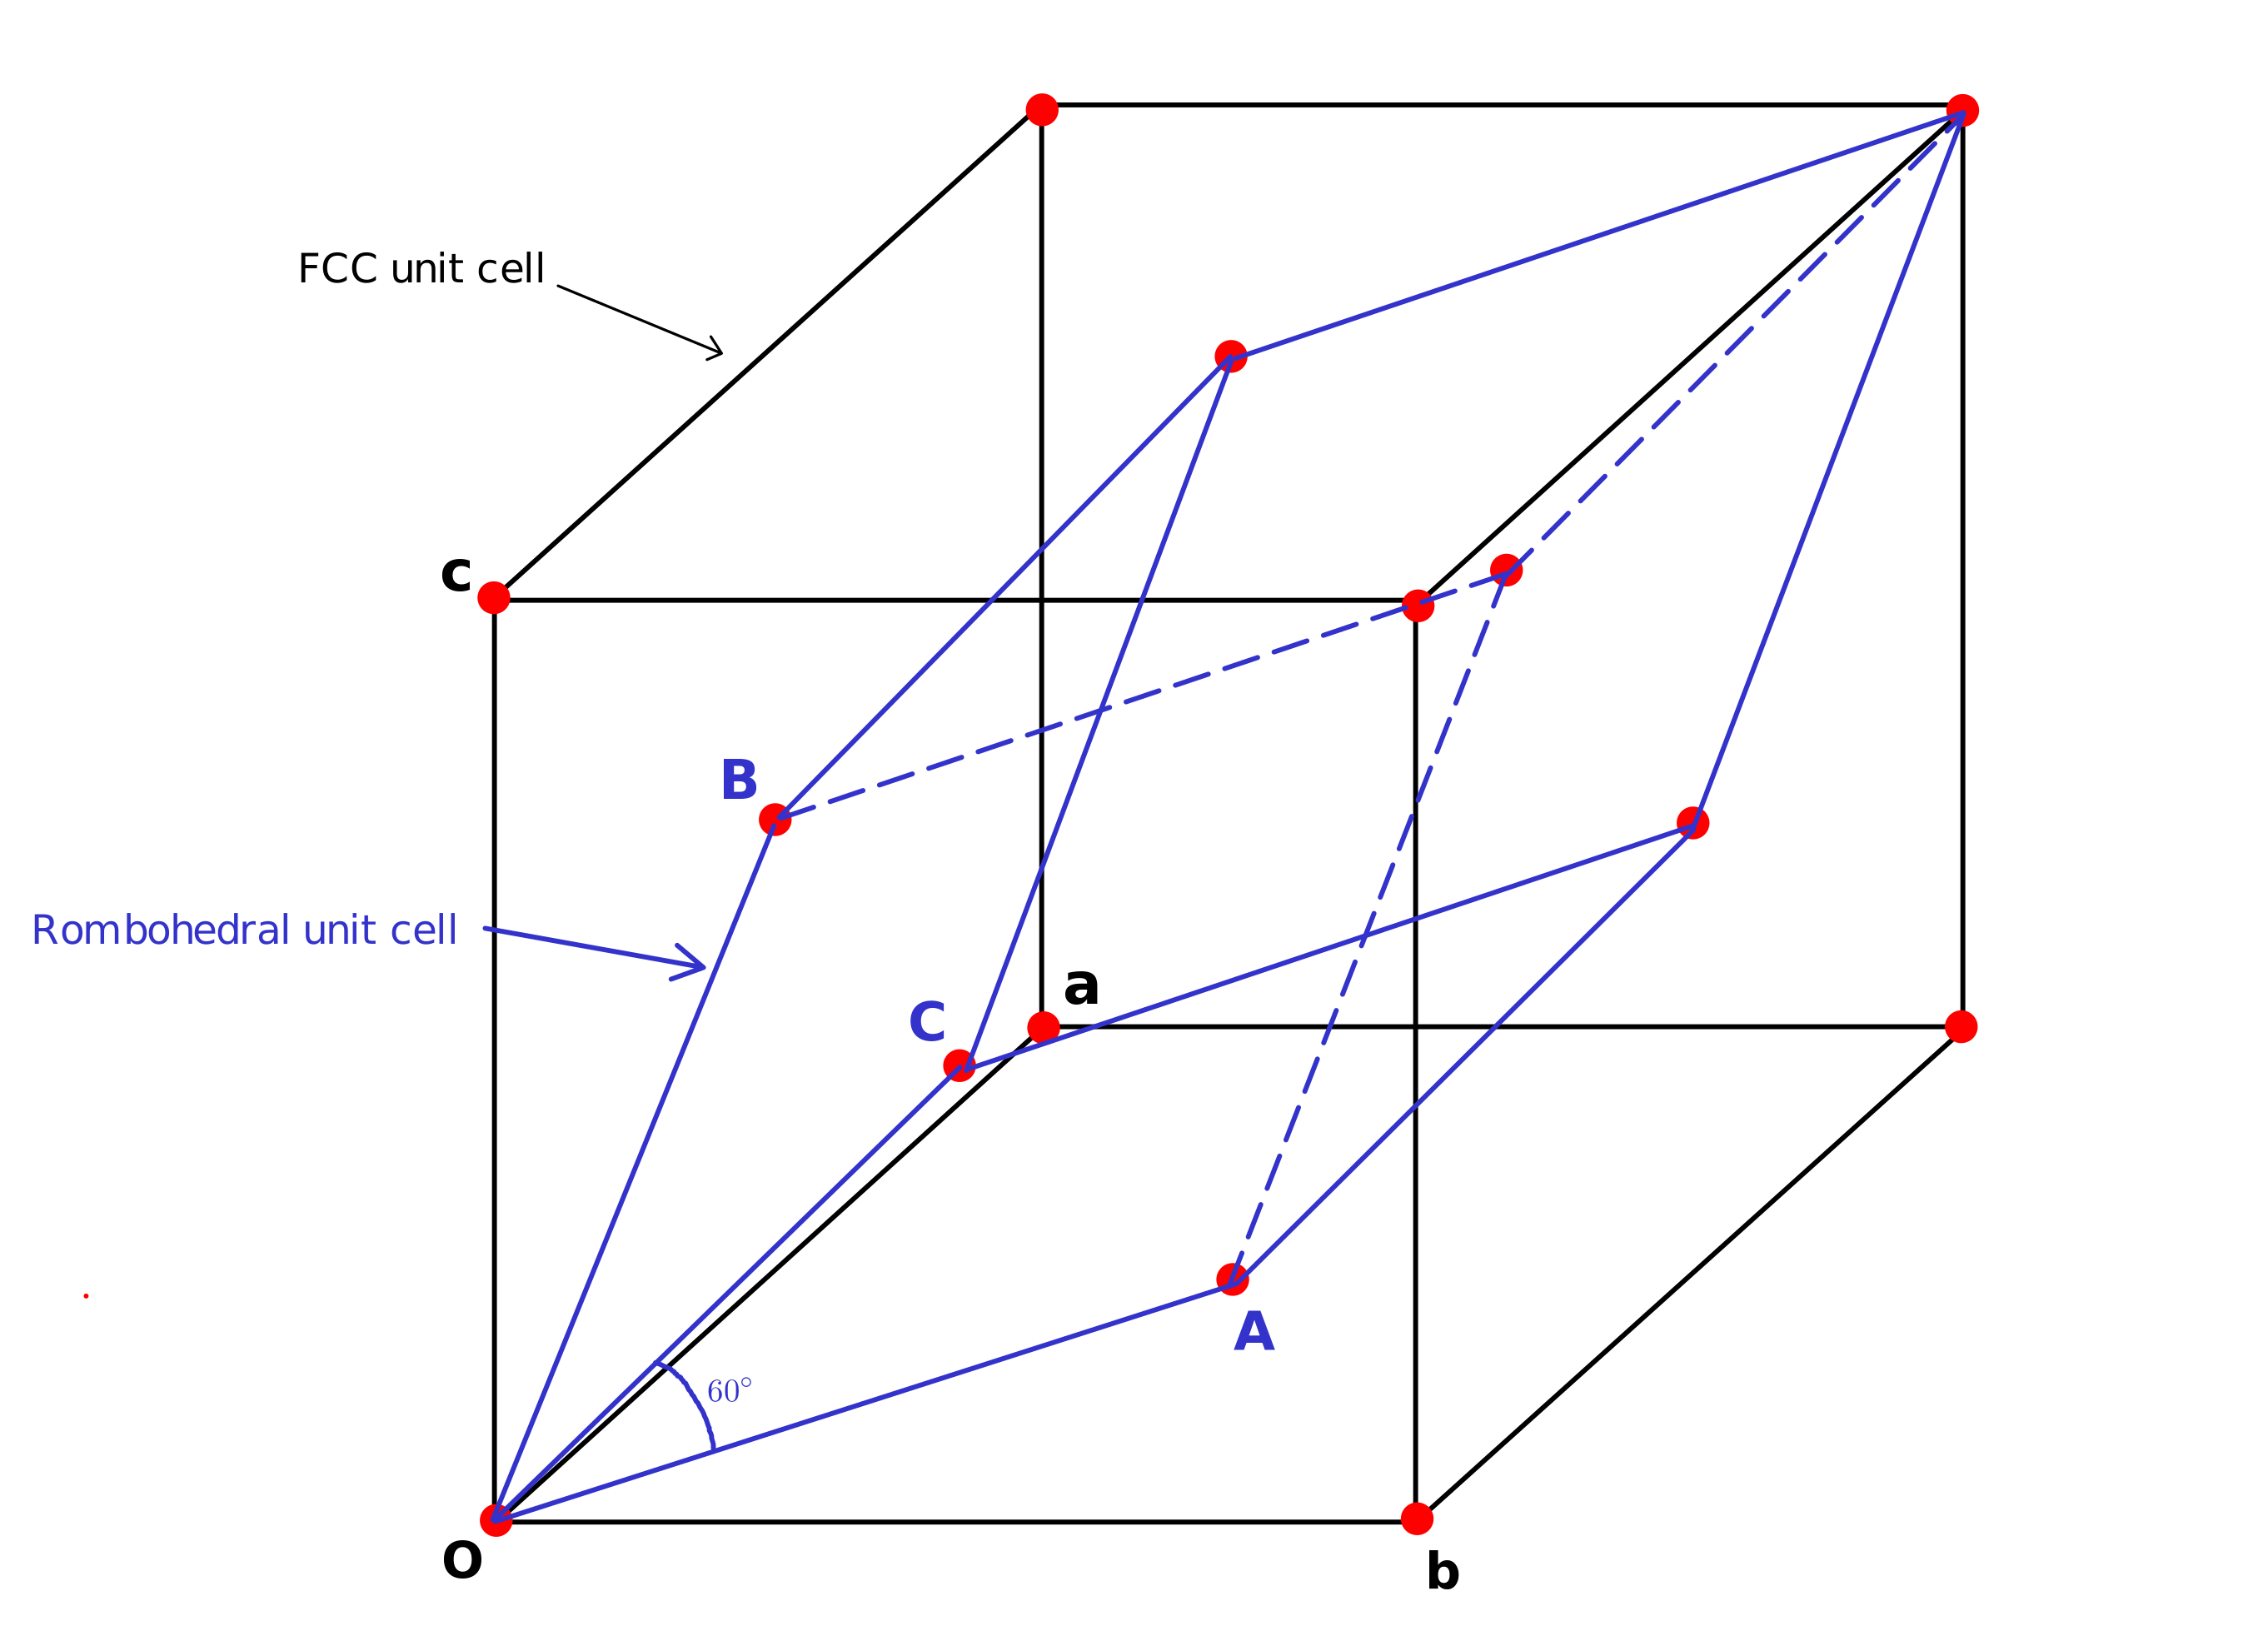
\includegraphics[scale=0.15]{fcc_lattice.png}
	\caption{\label{fig:fcc_fr}Cubic lattice with conventional face-centred unit cell, and a primitive rhombohedral unit cell.}
	\end{figure}
	
	Consider the cubic lattice shown in figure~\ref{fig:fcc_fr} with face-centred and rhombohedral unit cells. $\va{a}, \va{b}$ and $\va{c}$ are the basis vectors of the conventional FCC lattice, while $\va{A}, \va{B}$ and $\va{C}$ are the basis vectors of the primitive rhombohedral unit cell. The transformation equations are%
%		
	\begin{subequations}%
		\begin{align}
		\va{A} &= \frac{1}{2}\va{a} + \frac{1}{2}\va{b} + 0\va{c},\\[0.8em]
		\va{B} &= \frac{1}{2}\va{a} + 0\va{b} + \frac{1}{2}\va{c},\\[0.8em]
		\va{C} &= 0\va{a} + \frac{1}{2}\va{b} + \frac{1}{2}\va{c}.
		\end{align}
	\end{subequations}
	
	Miller indices follow the same transformation rules as unit cell vectors. Therefore,%
%	
	\begin{subequations}%
		\begin{align}
		H &= \frac{1}{2}h + \frac{1}{2}k + 0\ell \quad \implies 2H = h + k,\\[0.8em]
		K &= \frac{1}{2}h + 0k + \frac{1}{2}\ell, \quad \implies 2K = h + \ell,\\[0.8em]
		L &= 0h + \frac{1}{2}k + \frac{1}{2}\ell \quad \implies 2L = k + \ell.
		\end{align}
	\end{subequations}
	
	$\because H,K,L \in \mathbb{Z},$  $2H,\ 2K$ and $2L$ are all even integers, $\implies$ $h + k,\ h + \ell,$ and $k + \ell$ are also even integers.
	
	An even integer is the sum of either all odd or all even integers. Thus, reflections only occur from those lattice planes which have Miller indices $(hk\ell)$ all even or all odd. Planes for which the Miller indices are a mixture of off and even integers will be systematically absent in the X-ray diffraction peaks.
	
	Similar result can be derived using the structure factor equation, for body-centred cubic lattice, glide planes and screw axes.
	
%*********************************************************************************************

\subsection{Broadening of diffracted beams: the Scherrer equation}
	
	Till now, we have studied X-ray diffraction from a geometrical point of view. Incident and reflected beams were represented as perfectly collimated and narrow beams, and reflections occurred only at Bragg angles. This ideal situation is, in no way, the same as the practical situation as X-ray beams have a finite width and may not be perfectly parallel. Broadening of X-ray beams arise due to these instrumental factors. But, more importantly, inevitable line broadening arises from the crystallite size, perfection and state of strain of the specimen. The measurement of such broadening, after accounting for the instrumental factors, can give vital information about the specimen.
	
	The Scherrer equation is derived by considering a crystal of finite thickness $t$ perpendicular to the planes of interest, such that $m d){h k \ell} = t.$ Next, we consider interference conditions for incident and reflected beams that are slightly deviated, say by $\delta \theta,$ from the Bragg angle. As we go to higher order reflections, or equivalently, planes with larger Laue indices, the path difference due to this deviated angle adds up to finally result in a destructive interference. The condition for destructive interference for the whole crystal is obtained by pairing up the higher order reflections, and after some approximations, we arrive at the Scherrer equation:%
%		
	\begin{equation}
	\beta = \dfrac{K \lambda}{t \cos \theta}
	\end{equation}%
%	
	where $\beta$ is the full width of the Bragg peak at half the maxima (FWHM), and $K$ is often referred \cite{Klug1974} to as the crystallite shape factor. $K$ depends \cite{Holzwarth2011} on the crystallite shape, the definitions of average crystallite size and width. The structure of Scherrer equation is not affected by these, but the numerical value of $K$ can change appreciably. In the absence of detailed information about the shape of the crystal, $K = 0.9$ is a good approximation.
	
	The Scherrer equation becomes particularly useful when studying nanostructures because peak broadening becomes significant \cite{AkankshaUrade2023} when the crystallite size drops to $50-25~\si{nm}.$ At around $\SI{10}{nm},$ peak intensities become weak, and peak broadening becomes significant as peaks often overlap with each other, making it difficult to index and analyze the data.
	
	\section{The Choice of radiation}
	
	week 4, lec - 21 + week 5, lec - 22.
	
	\section{Type of X-ray diffraction experiments}

X-ray diffraction experiments for crystallography can be divided into two categories:%
%	
	\begin{itemize}%
%	
	    \item \bfnt{Powder XRD (PXRD)}:%
%	    	
	    	\begin{itemize}[label={$\rightarrowtail$}]%
%	    	
	    	    \item We get information about bulk properties like phase, purity, particle size, polymorph detection, etc.
	    	    
	    	    \item A bulk sample composed of micron or sub-micron sized particles is used.
	    	    
	    	    \item Small angle PXRD: $0-3~\si{\degree}$ in $2\theta.$ Wide angle PXRD: $3-80~\si{\degree}$ in $2\theta.$
	    	    
	    	    \item Generally, $\mathrm{Cu}~K_\alpha$ radiation is used.
	    	    
	    	\end{itemize}
	    	
	    \item \bfnt{Single Crystal XRD (SCXRD)}:%
%	    	
	    	\begin{itemize}[label={$\rightarrowtail$}]%
%	    	
	    	    \item Complete information about the crystal structure can be obtained.
	    	    
	    	    \item Slightly bigger crystals of size $5-50~\si{\micro\metre}$ have to be used.
	    	    
	    	    \item Generally $\mathrm{Mo}~K_\alpha$ radiation is used.
	    	    
	    	    \item $2-50~\si{\degree}$ in $2\theta$ sufficient for routine structure analysis. High resolution SCXRD requires $2\theta \in \qty[ \SI{2}{\degree}, \SI{120}{\degree} ].$
	    	    
	    	\end{itemize}
	    
	\end{itemize}
	
	\section{Single Crystal X-ray Diffraction}
	
	\subsection{\label{subsec:crystal_selection}Selection of crystals}

The criteria for selection of crystals for SCXRD is as follows:%
%			
	\begin{itemize}%
%			
	    \item \bfnt{Uniform internal structure}: The crystal should not have more than one domain of array of unit cells, should not be composed of a number of micron or sub-micron sized particles, and should not have crack or distortion of any means. However, \ifnt{the crystal need not have well-defined faces}.
	    
	    \item \bfnt{Suitable size and shape}: For SCXRD experiments, chosen crystals should have dimensions in the range $50-500~\si{\micro\metre}.$ The size of the crystal must be smaller than the spot size of the X-ray beam.
	    
	    \begin{figure}
	    	\centering
	    	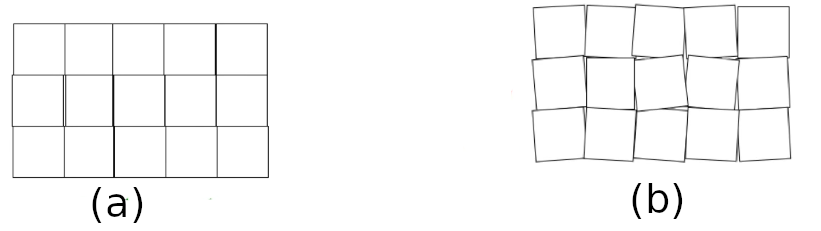
\includegraphics[scale=0.5]{imperfect_crystal.png}
	    	\caption{\label{fig:imperfect_crystal}The crystal on the left is a perfect crystal. The one on the right is a mosaic crystal with a deviation of $\sim 0.1-0.2 \si{\degree}.$ Image courtesy:~\cite{Chowdhury2022}.}
	    \end{figure}
	    
	    \item \bfnt{Imperfect crystals are better.} In perfect crystals, lattice planes traverse in the whole crystal without any deviation, resulting into extinction. Majority of crystals are imperfect, and they diffract better than perfect crystals. Imperfectness may be deliberately introduced into a crystal by a shock.
	    
	    \begin{figure}
	    	\centering
	    	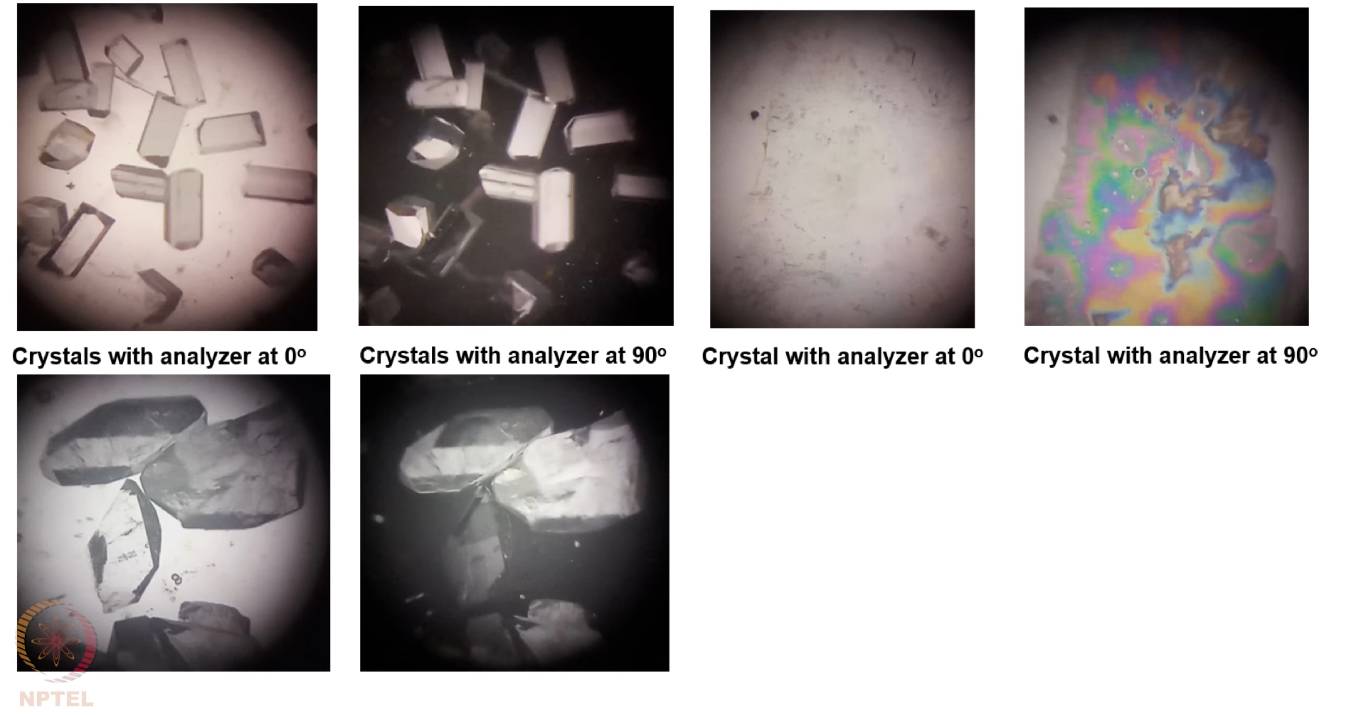
\includegraphics[scale=0.4]{crystal_optical_microscope.png}
	    	\caption{\label{fig:crystal_optical_micro}Crystals when viewed through an optical microscope in polarized light. The set of crystals on the left are good crystals because they are either uniformly dark or uniformly bright when the analyzer is rotated by $\pi/2.$ The crystal on the right shows different colours when the analyzer is rotated, implying that it has more than one domain and cannot be studied under SCXRD. Image courtesy:~\cite{Chowdhury2022}.}
	    \end{figure}
	    
	    \item \bfnt{Screening under optical microscope for domains}: Polarized light is passed through a crystal, and the crystal is rotated about its axis. The transmitted light is observed through an analyser. If, on rotating the analyser, the crystals appears either uniformly dark or uniformly bright in all regions of the crystal, then the crystal has a single domain. Crystals with multiple domains would appear both dark and bright, or show multiple colours at certain angles between the polariser and analyser. This is demonstrated in figure~\ref{fig:crystal_optical_micro}.
	    
	\end{itemize}
	
		We cannot know whether a crystal is good or bad until we mount it on the diffractometer and put it in the path of X-rays. Therefore, when a crystal passes the above minimum selection criteria, we mount it on the goniometer head and shine X-rays on it. The axis about which the crystal is mounted is known as the $\phi$ axis. We rotate crystal about the $\phi$ axis through a full $2\pi$ rotation while keeping the X-ray on for 1-2 minutes depending on the size of the crystal, and we keep recording the diffraction pattern. The diffraction pattern thus recorded is known as the \bfnt{rotation photograph} of the single crystal.
	
	\begin{figure*}
	\centering
	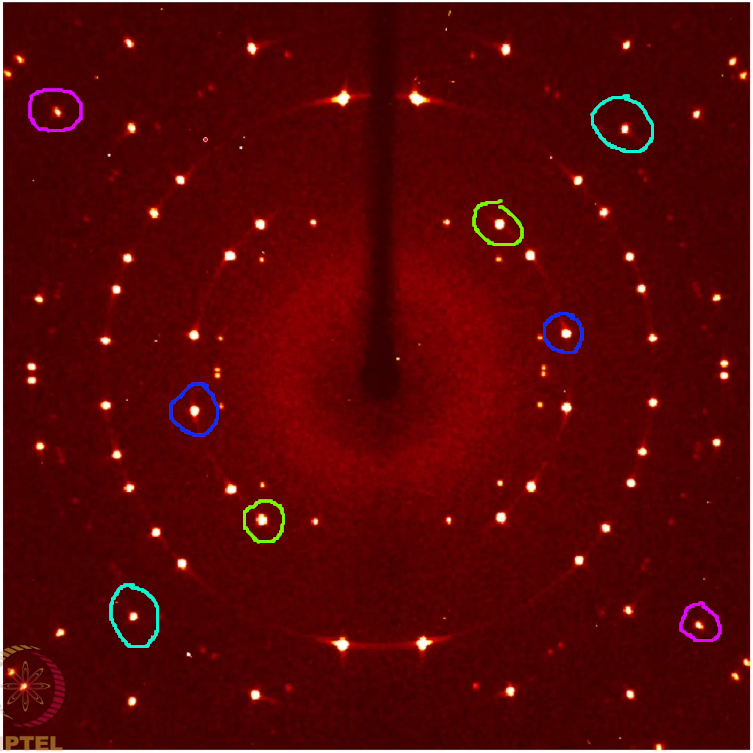
\includegraphics[scale=0.3]{rotation_photograph_mod.png}
	\caption{\label{fig:rotation_photo}Rotation photograph of a single crystal of $\mathrm{NaCl}$. Each spot has another spot on the other side related by a centre of inversion. Some examples are shown by different coloured circles; two spots encircled by the same colour are related to each other. The dark shadow is that of the beam stop, which prevents the direct X-ray beam from falling on the detector. Image courtesy:~\cite{Chowdhury2022}.}
	\end{figure*}
	
	Figure~\ref{fig:rotation_photo} shows the rotation photograph of a single crystal. This photograph is always centrosymmetric irrespective of the type of crystal geometry. Each spot on the rotation photograph has another corresponding spot that is related to it by a centre of inversion. If instead of these spots, the rotation photograph is composed of concentric circles, we conclude that the crystal is not a single crystal, but a polycrystal, and is not suitable for XRD.
	
	\section{Mounting a crystal on SCXRD diffractometer}

	\begin{figure*}[t]
		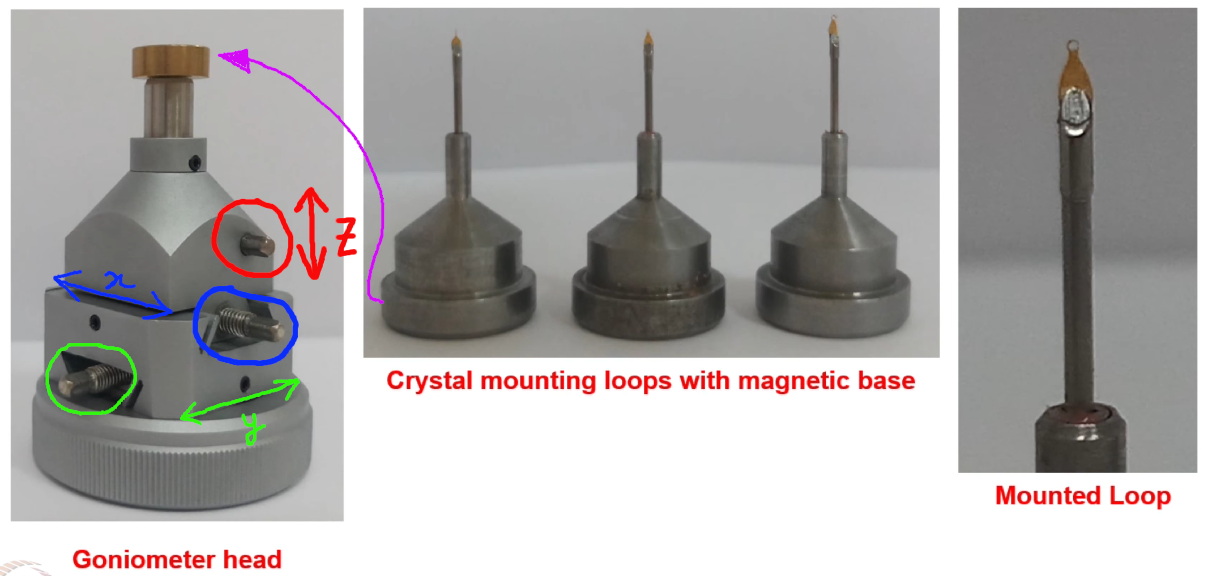
\includegraphics[scale=0.5]{goniometer_mod.png}
		\caption{\label{fig:goniometer}The goniometer head, mounting loop with the mounting base.}
	\end{figure*}

	In fig.~\ref{fig:goniometer}, a goniometer head is shown. This head is mounted on the goniometer of the diffractometer. The top of the goniometer head is a magnetic base which allows the mounting loops to be held in place. To align the crystal in the X-ray beam, the goniometer head has three screws that allow movement in the three Cartesian directions. These screws and their respective directions have been demarcated in the figure.

		The tip of the mounting metal pin has a small polymer loop. The crystal is mounted on this loop using some thick oil, which keeps the crystal in place by its surface tension. These loops are available in various diameters, generally in the range $0.05-0.5~\si{mm}.$

		Nylon loops are also available, in which the loop is made by a nylon thread, which is then twisted several times and then glued to a pin. The pin is attached to a brush, which can be directly mounted on the goniometer head and placed in the X-ray beam.

	\subsection{The diffractometer}

\begin{figure}
	\centering
	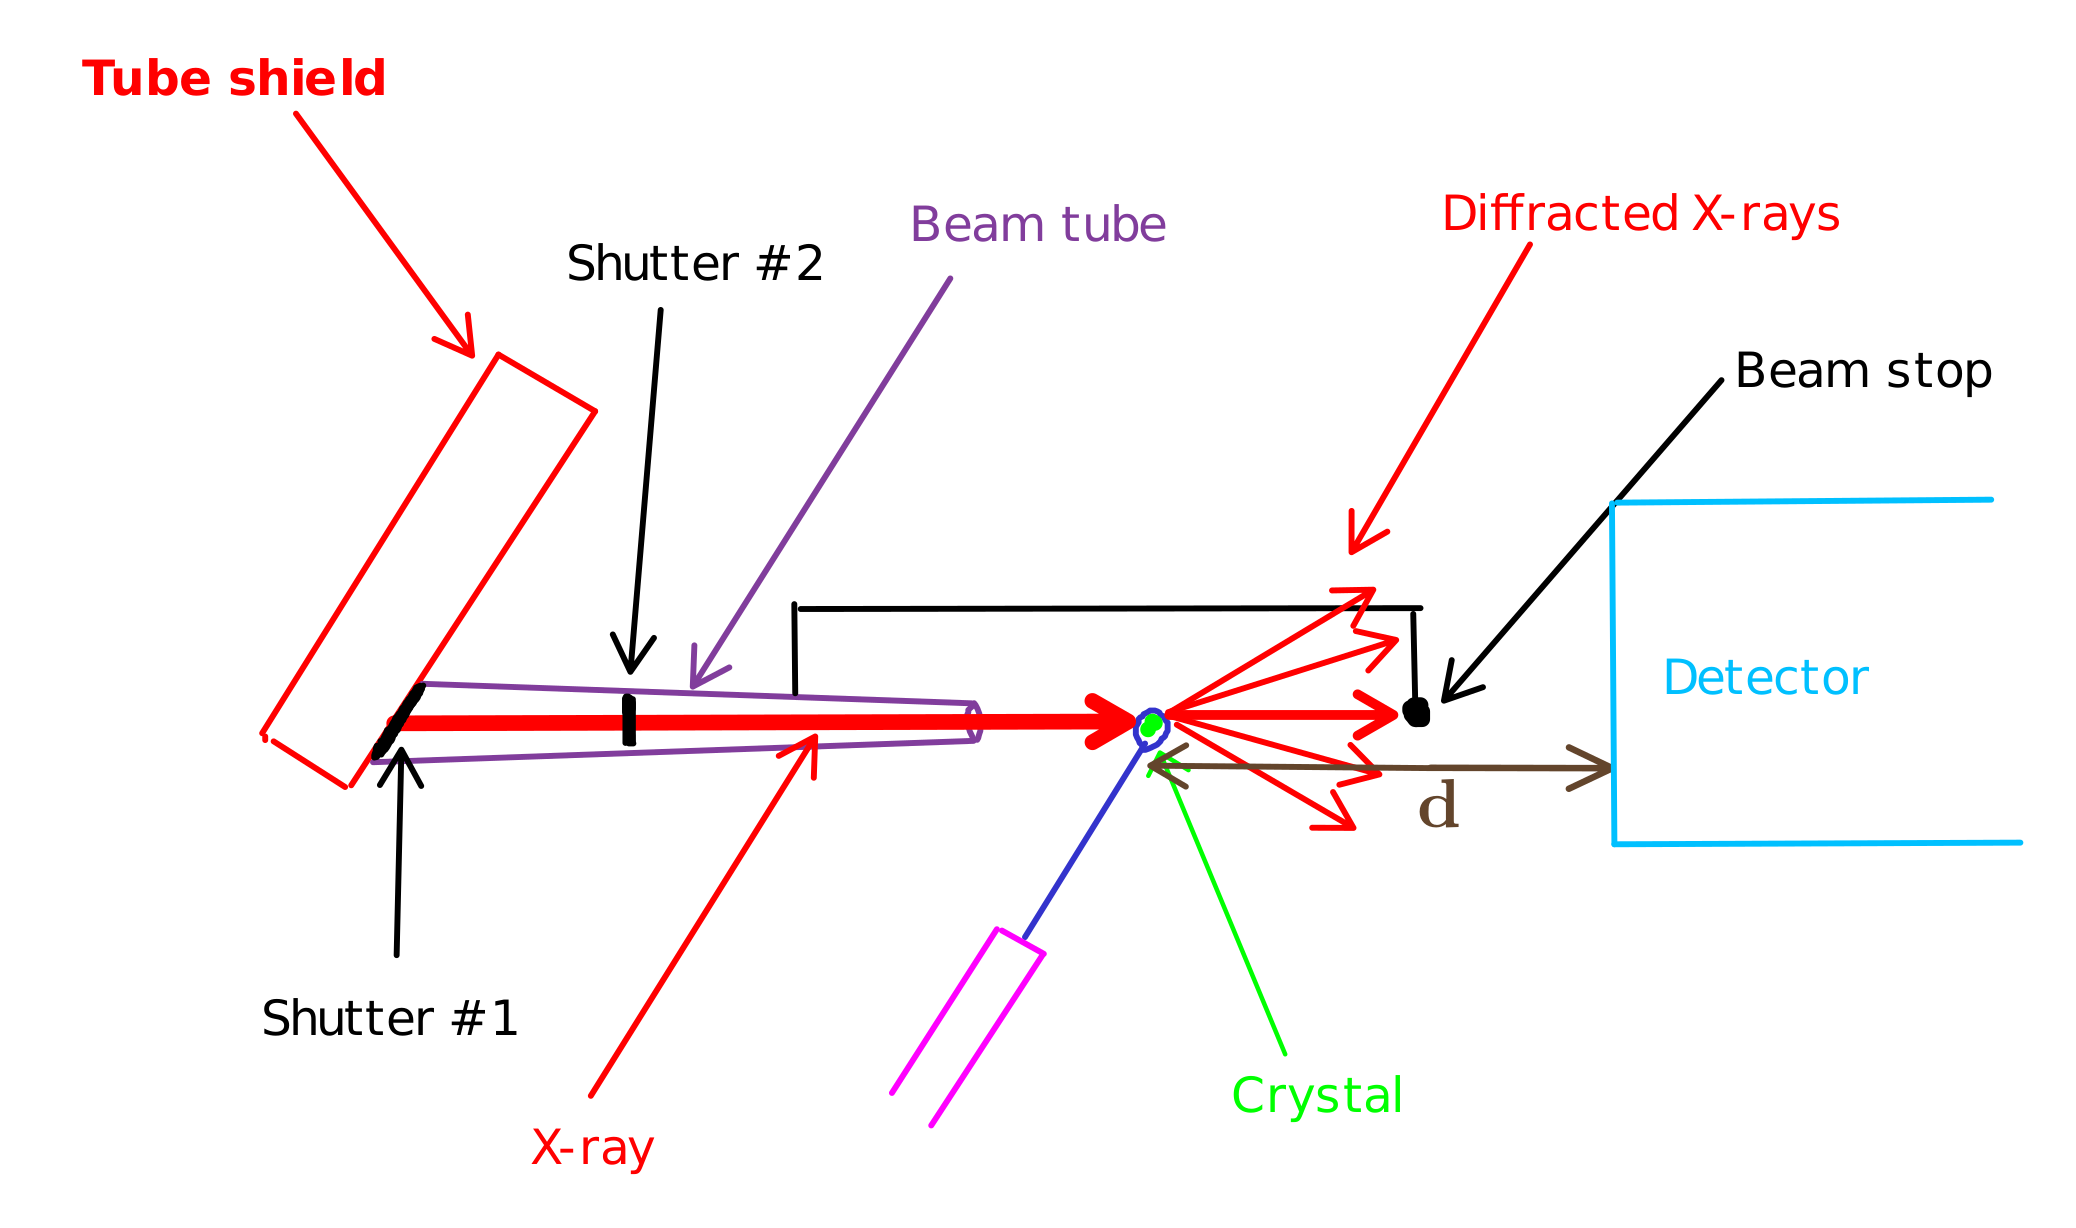
\includegraphics[width=\textwidth]{sc_diffractometer_lateral.png}
	\caption{\label{diffractometer_lateral}Lateral view of a SCXRD diffractometer. See text for details.}
\end{figure}

Figure~\ref{diffractometer_lateral} is a lateral schematic of the diffractometer. The X-rays are generated within the tube shield and are emitted through the transparent Be window. When we physically work with the diffractometer, for example, to mount the crystal, we do not want the X-rays in the diffractometer chamber. Shutter \# 1 on the tube shield is used to stop the X-rays from coming out of the tube shield. The beam pipe contains the beam optics, which consists of the $K_\beta$ filter, collimation optics, as well as another shutter. This shutter controls the exposure time.

The intensity of the generated X-rays is very high, and all of the intensity is not diffracted by the crystal. A portion of the X-ray beam transmits through the crystal and directly hits the detector if it is at $2\theta = 0.$ This high intensity beam can damage the detector. The beam stop prevents the direct beam from falling on the detector. For a typical beam of spot size $\SI{0.5}{mm}$ diameter, the beam stop is $\sim \SI{2}{mm}.$ In Fig.~\ref{fig:rotation_photo}, the dark portion is the shadow of this beam stop.

The distance between the detector and the crystal, denoted by $d,$ is generally kept $4-10~\si{cm},$ and the detector can move back upto $\SI{18}{cm}.$ The intensity of the diffracted beam falls off $\propto \dfrac{1}{d^6}.$ Hence, if $d$ is large, exposure time will increase. $d$ depends on the lattice parameters of the crystal:%
%	
	\begin{subequations}
		\begin{align}
		d \sim \begin{cases}
		\SI{4}{cm} & \text{for } a, b, c < 12-13~\si{\angstrom};\\
		5-6~\si{cm} & \text{for } a, b, c < 12-30~\si{\angstrom};\\
		7-8~\si{cm} & \text{for } a, b, c > \SI{30}{\angstrom}.\\
		\end{cases}
		\end{align}
	\end{subequations}
	
\begin{figure}
	\centering
	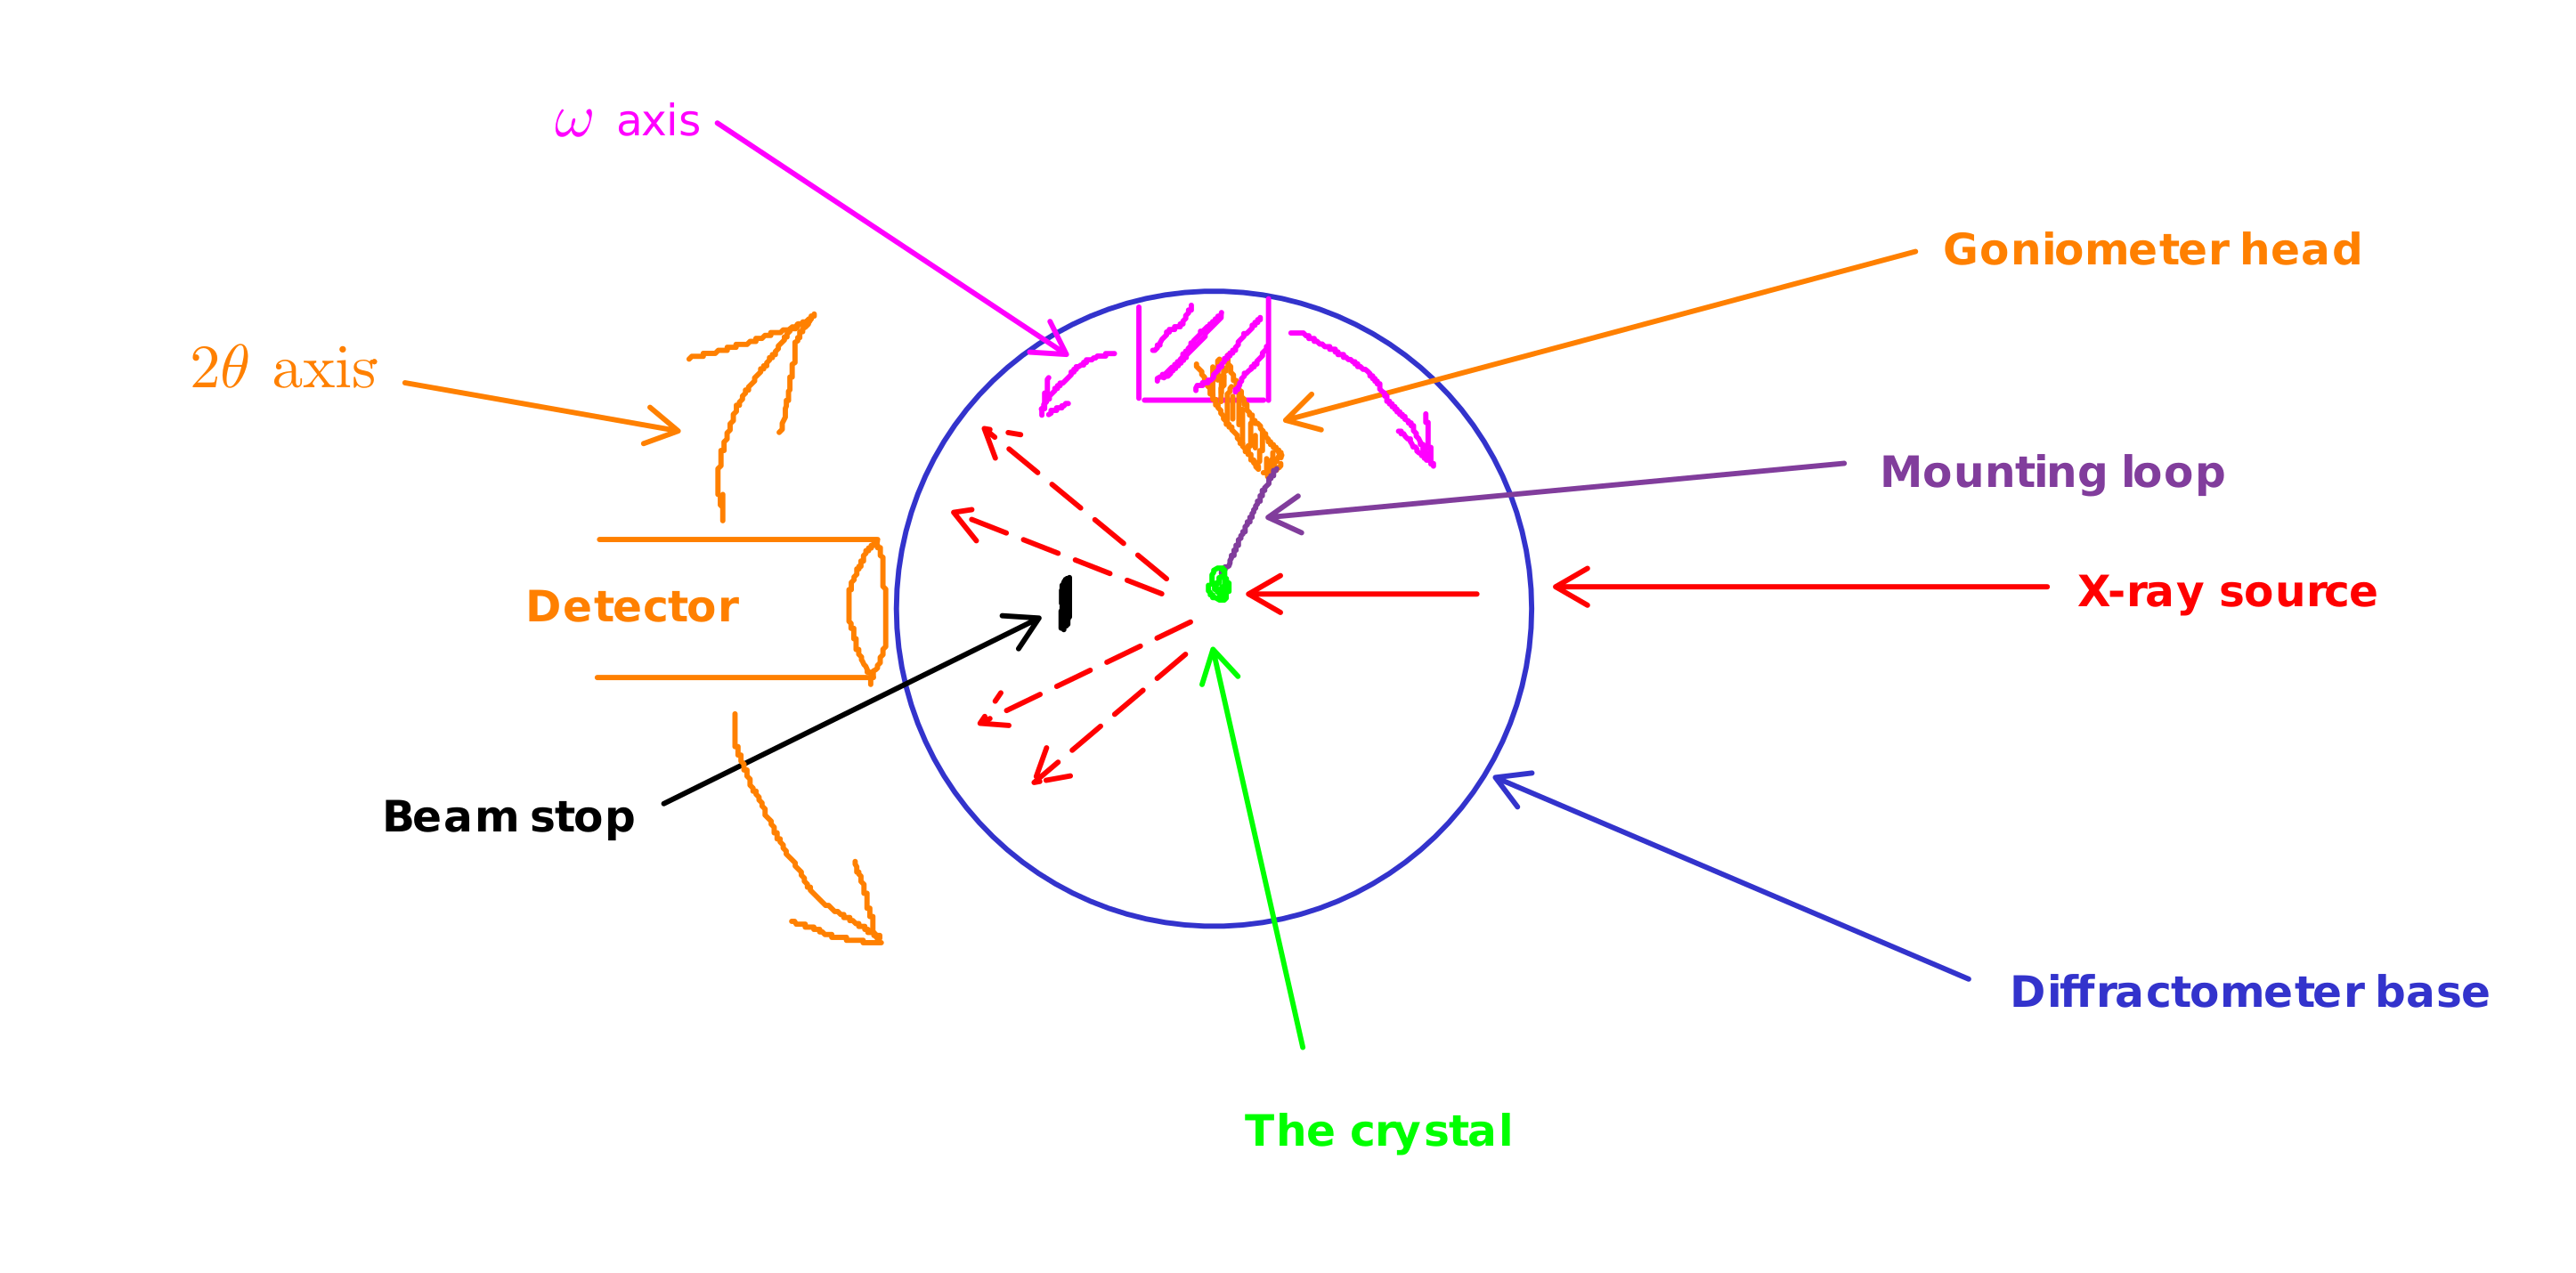
\includegraphics[width=\textwidth]{sc_diffractometer_omega.png}
	\caption{\label{diffractometer_omega}Top view of a SCXRD diffractometer. The $\omega$ axis is the rotation axis of the diffractometer base. $2\theta$ is the angle of rotation of the detector.}
\end{figure}
	
\begin{figure}
	\centering
	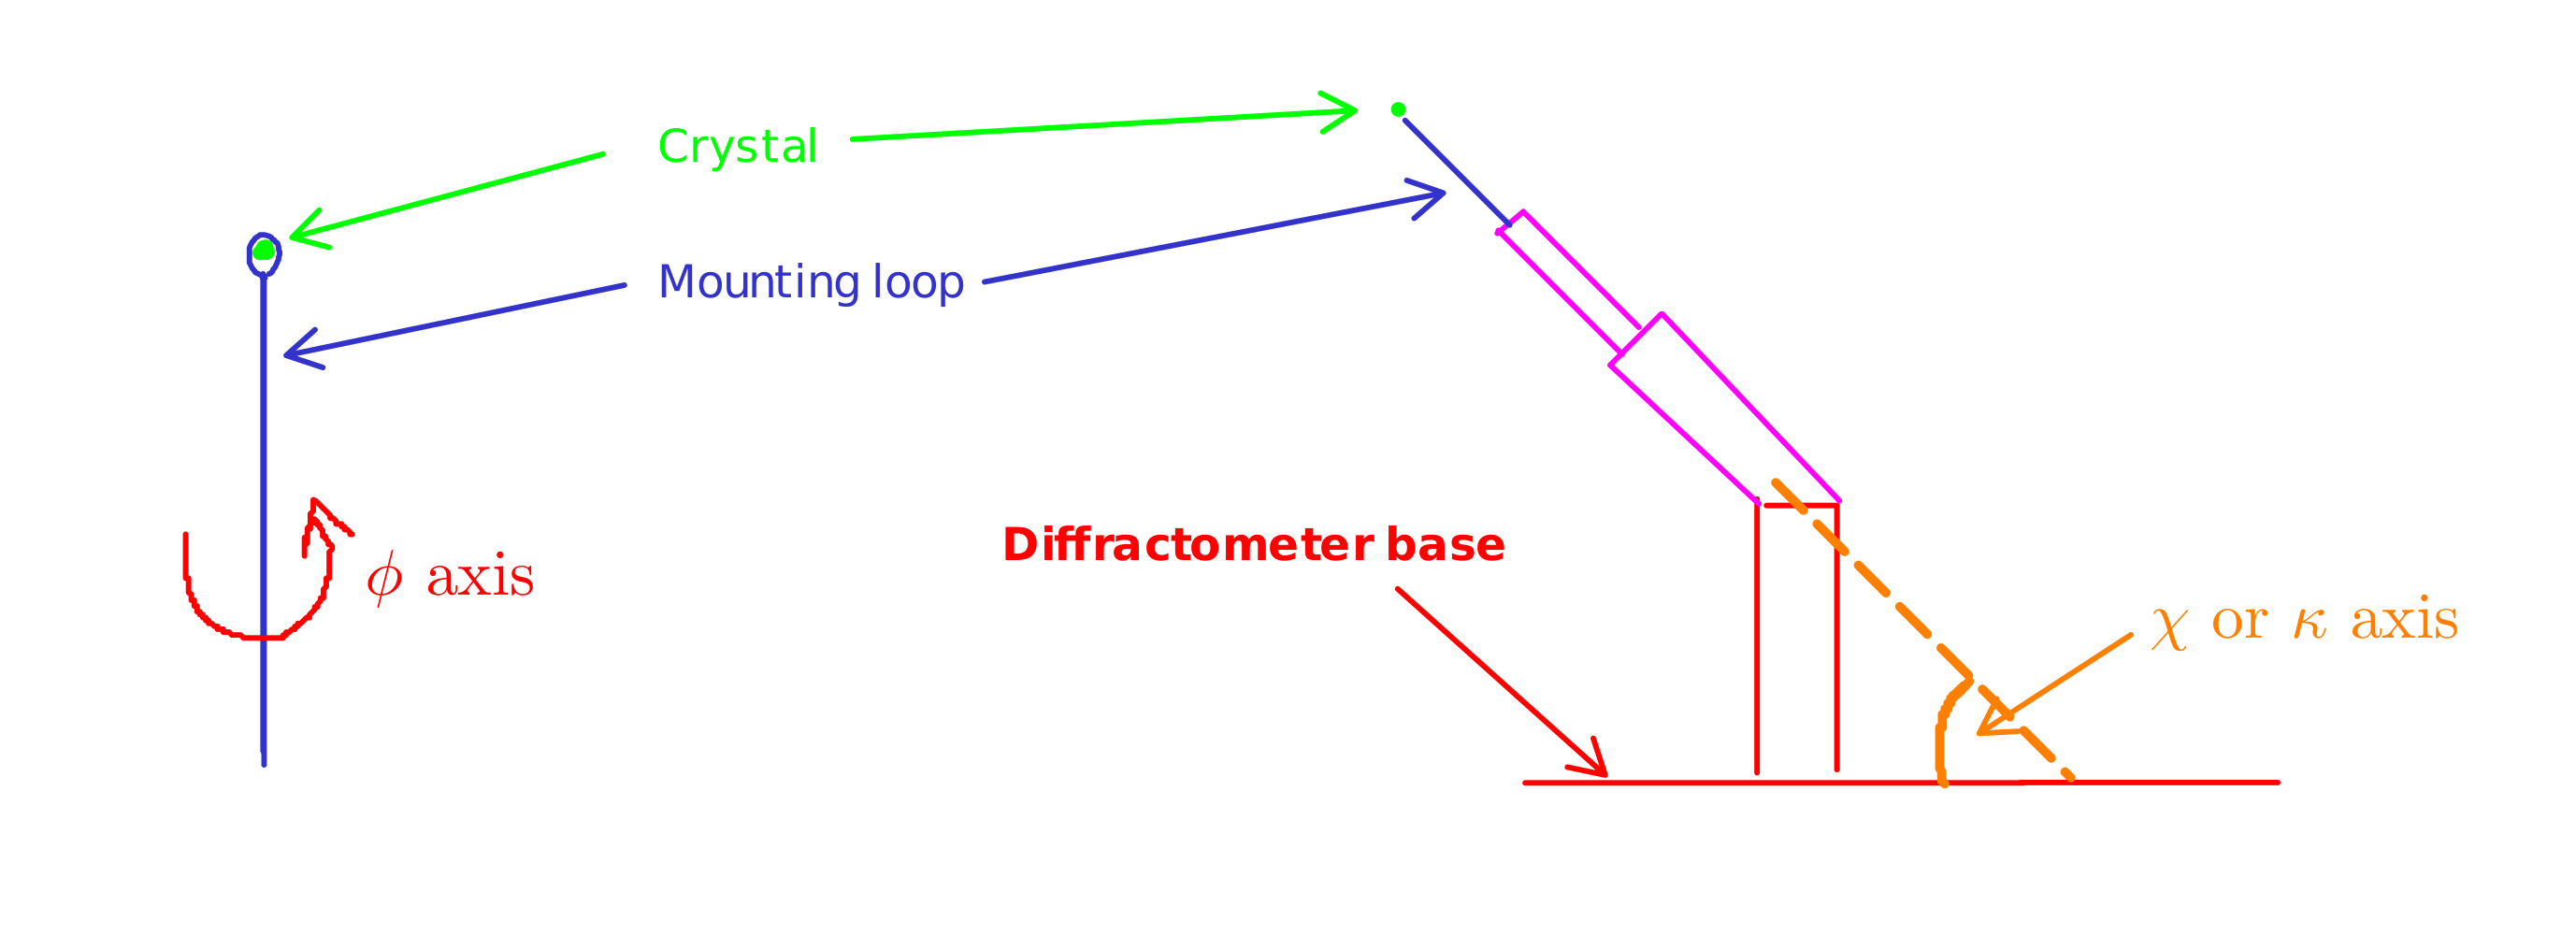
\includegraphics[width=\textwidth]{sc_diffractometer_phi_chi.png}
	\caption{\label{diffractometer_phi_chi}The $\phi$ axis is the rotation axis of the crystal about the mounting loop. If the angle that the goniometer makes with the diffractometer base is fixed, then the angle is termed as the $\chi$ axis, with $\chi = \SI{54.7}{\degree}.$ If this angle can be changed, then the same axis is known as the $\kappa$ axis.}
\end{figure}

\begin{figure}
	\centering
	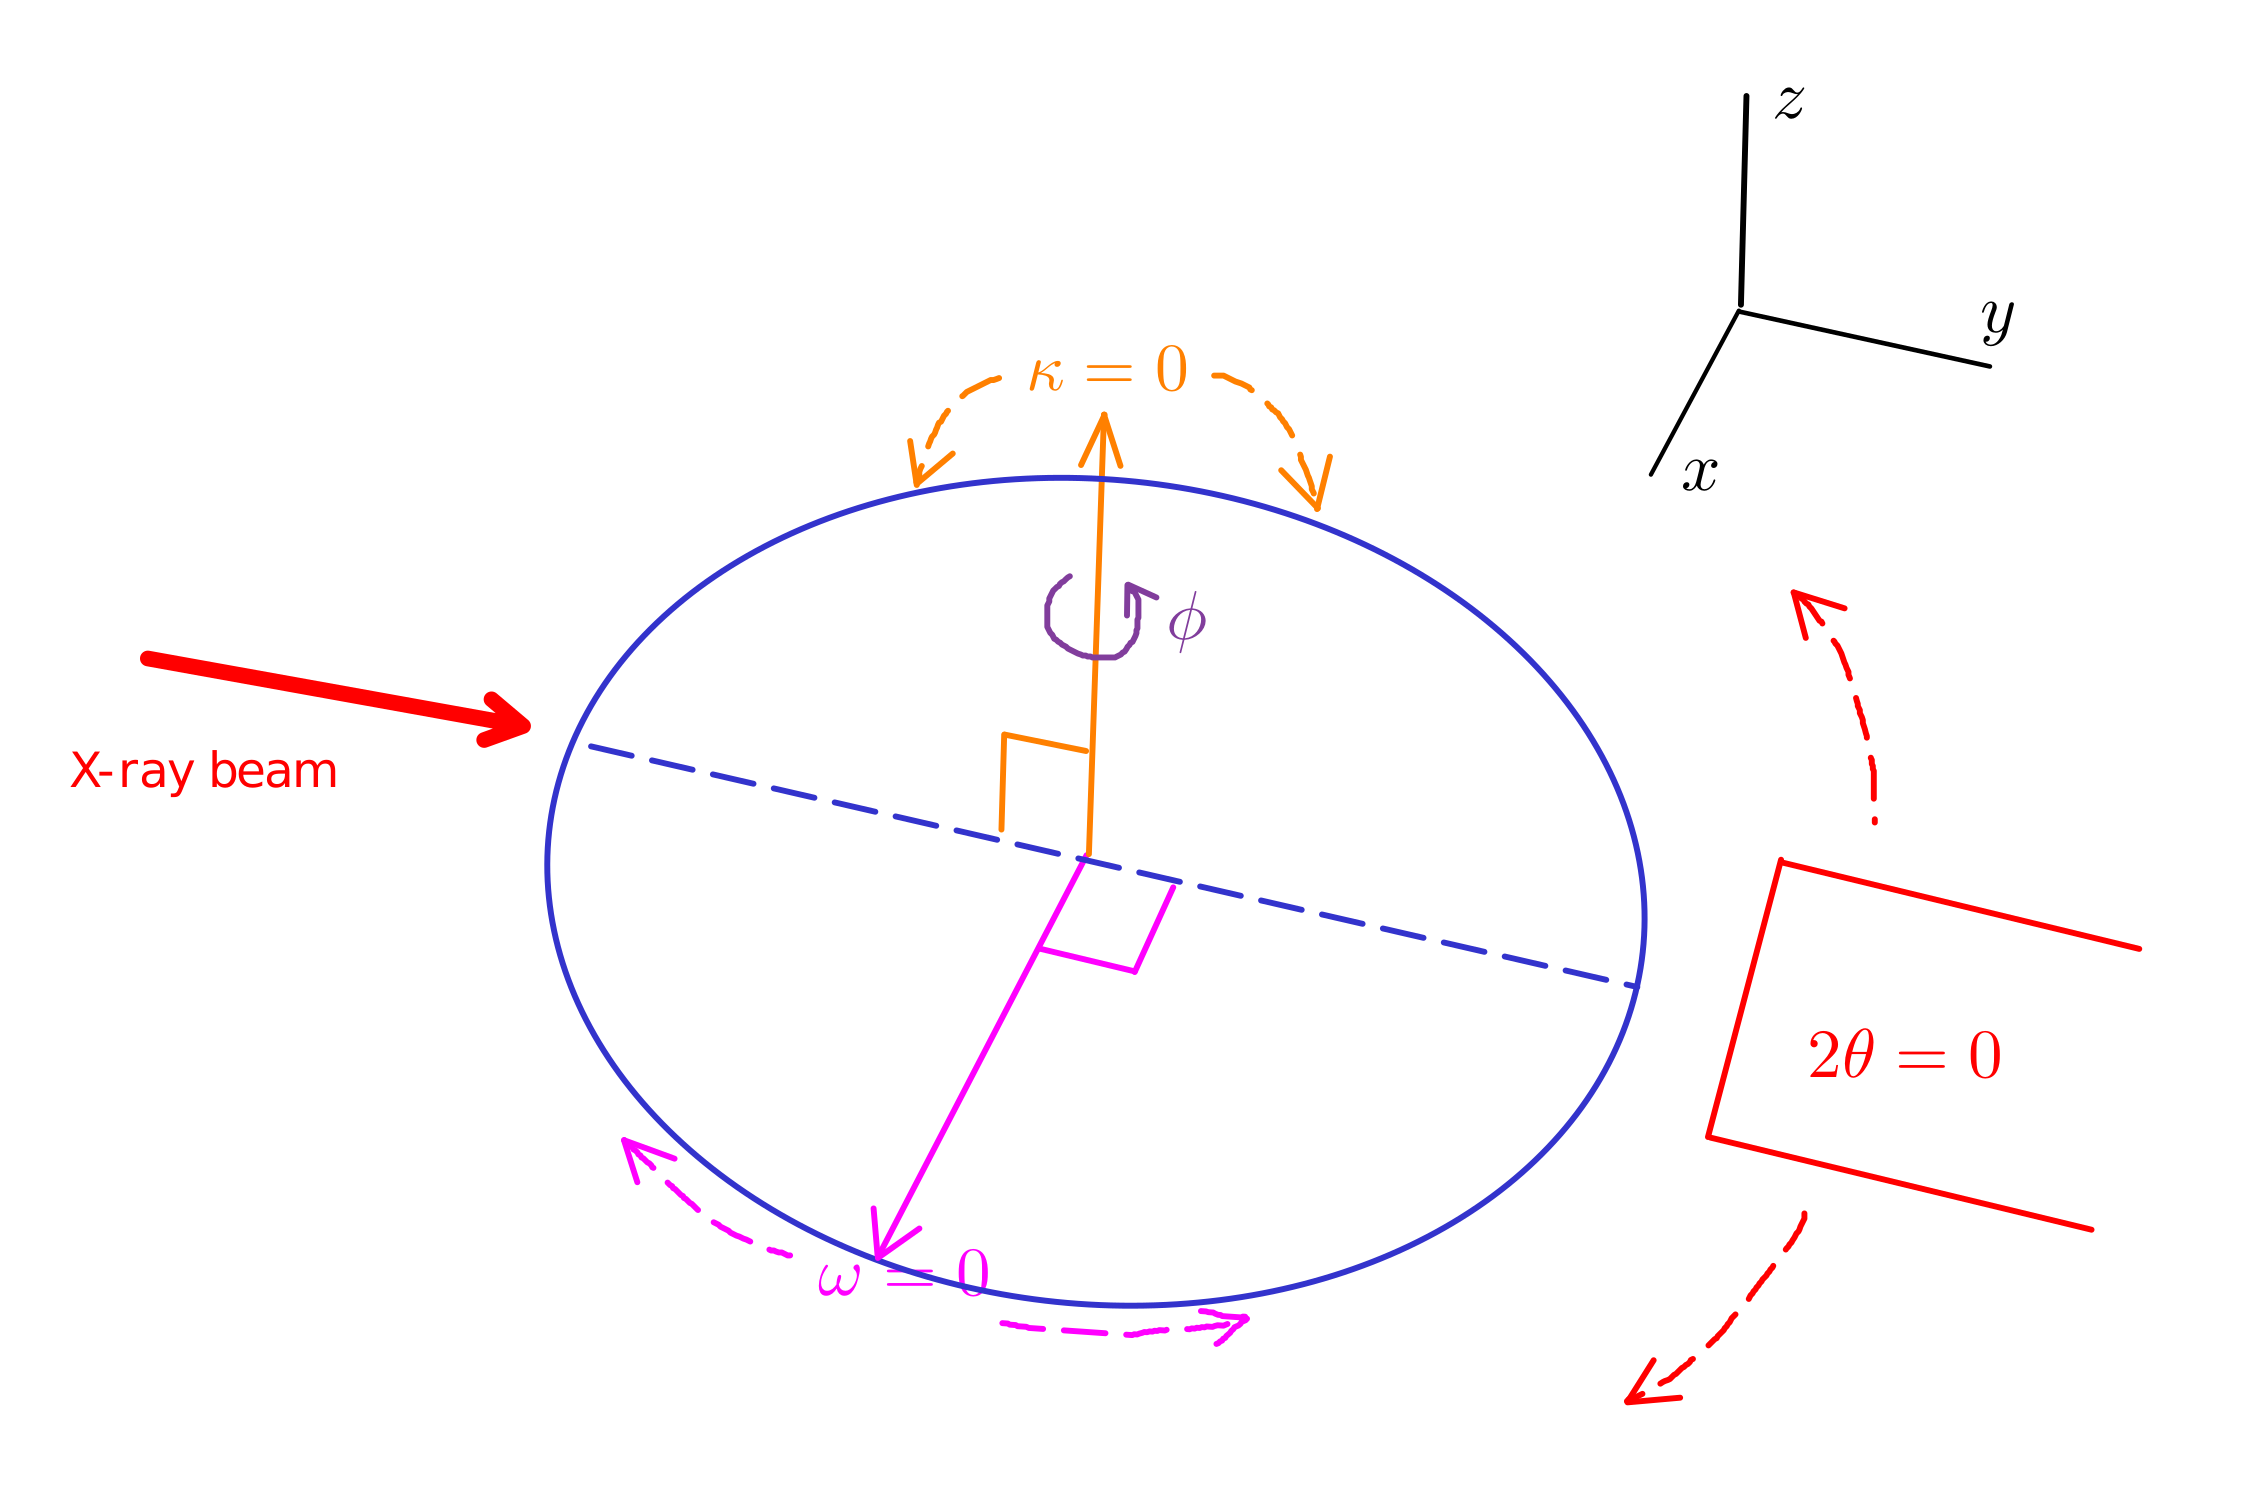
\includegraphics[width=\textwidth]{all_axes.png}
	\caption{\label{diffractometer_all_axes}All the axes of a single crystal diffractometer.}
\end{figure}
 
A diffractometer can have four axes of rotation:%
%	
	\begin{enumerate}%
%	
	    \item $\phi$ axis,
	    
	    \item $\omega$ axis,
	    
	    \item $\chi$ or $\kappa$ axis, and
	    
	    \item $2\theta$ axis.
	    
	\end{enumerate}

These axis are shown in figures~\ref{diffractometer_omega}, \ref{diffractometer_phi_chi} and \ref{diffractometer_all_axes}.\\

Based on this, SCXRD diffractometers can be classified into:%
%	
	\begin{itemize}%
%	
	    \item \ul{2-circle diffractometer}: $\phi$ and $\omega$ can be varied, but $\chi$ and $2\theta$ are fixed. $2\theta$ is fixed at $\SI{30}{\degree}.$ But the coverage area of the detector is such that if it sits at $\SI{30}{\degree},$ it can actually reach $0-60\si{\degree}.$ For $\mathrm{Mo}~K_\alpha$ radiation, the IUCr prescribed minimum $2\theta = \SI{50}{\degree}.$ So, a 2-circle diffractometer works fine for $\mathrm{Mo}~K_\alpha$ radiation. We can, however, not go to higher angles, so this diffractometer is used for routine analysis of crystals.
	    
	    \item \ul{3-circle diffractometer}: $\phi$, $\omega$ and $2\theta$ can be varied. Allows data recording upto high angles.
	    
	    \item \ul{4-circle diffractometer}: $\phi$, $\omega$, $2\theta$ and $\kappa$ can be changed. Reduces data collection time because a large number of reflections can be brought to the periphery of the Ewald sphere.
	    
	\end{itemize}
	
\begin{table}
	\newcounter{sl_no}
	\centering
	\caption{\label{tab:3_circ_diff_angles}Standard measurement angles and exposure time for a 3-circle diffractometer. $\Delta \omega$ is the step size or width in $\omega.$ The full set represents a complete sphere of data; the first two sets are recorded with 200 frames of the third set correspond to a hemisphere of data.}
	\begin{tabular}{|c|C|C|C|C|C|C|C|}
		
		\hline
		
		Sl. No. & 2\theta & \omega & \phi & \multicolumn{1}{c|}{\makecell{$\chi$\\(Fixed)}} & \Delta \omega & \multicolumn{1}{c|}{\makecell{\text{No. of frames}}} & \multicolumn{1}{c|}{\makecell{\text{Exposure time}\\$t$ (in s)}}\\
		
		\hhline{|=|=|=|=|=|=|=|=|}
		
		\stepcounter{sl_no}\arabic{sl_no} & \SI{-30}{\degree} & \SI{-30}{\degree} & 0 & \SI{54.74}{\degree} & \SI{1}{\degree}/\SI{0.5}{\degree}/\SI{0.3}{\degree} & 180/360/600 & 5/10/15\\
		
		\hline
		
		\stepcounter{sl_no}\arabic{sl_no} & \SI{-30}{\degree} & \SI{-30}{\degree} & \SI{90}{\degree} & \SI{54.74}{\degree} & \SI{0.3}{\degree} & 600 & 10\\
		
		\hline
		
		\stepcounter{sl_no}\arabic{sl_no} & \SI{-30}{\degree} & \SI{-30}{\degree} & \SI{180}{\degree} & \SI{54.74}{\degree} & \SI{0.3}{\degree} & 600 & 10\\
		
		\hline
		
		\stepcounter{sl_no}\arabic{sl_no} & \SI{-30}{\degree} & \SI{-30}{\degree} & \SI{270}{\degree} & \SI{54.74}{\degree} & \SI{0.3}{\degree} & 600 & 10\\
		
		\hline
	
	\end{tabular}
\end{table}

	
Data collection strategies vary based on the type of diffractometer and the crystal being studied. Table~\ref{tab:3_circ_diff_angles} lists the standard angles which allow a full sphere of data to be collected using a 3-circle diffractometer. The exposure time is the time period for which the X-ray is allowed to fall on the crystal before its orientation is changed. The crystal is not kept stationary, instead, it is slowly rotated about the $\omega$ axis in steps of $\Delta\omega.$ A large value of $\Delta\omega$ implies that we are slicing the reciprocal lattice into wider slices. If we take $\Delta\omega = \SI{1}{\degree},$ it is recommended that we use a larger exposure time, so that the exposure time per degree remains fixed. Smaller values improve the quality of data. If $\chi$ (i.e. $\kappa$) can be varied, we can get the data faster.

Diffractometers have pre-fixed strategies that are used when an unknown crystal is loaded for the first time. This strategy cannot be edited, but may be extended in some cases. Using this strategy, 20-30 frames are recorded, from which the diffractometer informs us about the lattice parameters $a, b, c, \alpha, \beta$ and $\gamma,$ and the type of lattice (P, I, F, C). From the lattice parameters, we can get the volume of the unit cell, $V.$ $V / Z$ is the volume of the asymmetric unit, i.e. the smallest unit cell that can be used to represent the lattice. This asymmetric unit must contain the total number of atoms.

Let $n$ be the number of non-Hydrogen atoms present in the molecule of interest.%
%
\begin{equation}
\therefore \text{Average atomic volume} = \dfrac{V}{Zn}.
\end{equation}

This average atomic volume should range between $16-20~\si{\angstrom}.$ If the measured value does not fall within this range, we have to check if the asymmetric unit has solvents, and take into account the number of Hydrogen atoms in the solvent. If the value still does not match, we have to discard the crystal and start over again.
	
	\subsection{Detectors}

Three types of detectors are available: charge coupled devices (CCD), CMOS and Direct Photon Counting Detectors.

CCD and CMOS contain photo sites or pixels. When light falls on a pixel, charge accumulates, which gives rise to a potential difference. This potential difference is amplified and then recorded.

In CCD, the pixels are read column-wise one after the other. Hence, it takes time to read all the pixels. CMOS technology, on the other hand, can simultaneously read data from all pixels. Hence, CMOS is preferred over CCD.

Temperature plays a significant role in the quality of data collected. If we carry out the XRD at room temperature of $\sim \SI{300}{K},$ the latice ions will vibrate in all the three directions due to thermal energy. Thus, the electron density associated with each of those atoms will be largely diffused over the plane of the atom. Due to this, the electron planar density is decreased and the diffraction will be weak. Therefore, we generally carry out XRD at $\SI{100}{K}$ using liquid nitrogen cryogen, or at $6-10~\si{K}$ using liquid He.
	
	\subsection{How much data do we have to collect?}

\textbf{Friedel's Law} states that the intensity of diffracted beam from $(hk\ell)$ set of planes and $(\bar{h} \bar{k} \bar{\ell})$ set of planes is equal. Mathematically,%
%	
	\begin{equation}
	I_{hk\ell} = I_{\bar{h} \bar{k} \bar{\ell}}.
	\end{equation}
	
This stems from the fact that the $(hk\ell)$ set of planes is actually the same as the $(\bar{h} \bar{k} \bar{\ell})$ set of planes, with the latter being seen from a different origin. Friedel's Law holds irrespective of whether the crystal is centrosymmetric or not.

\begin{figure}
	\centering
	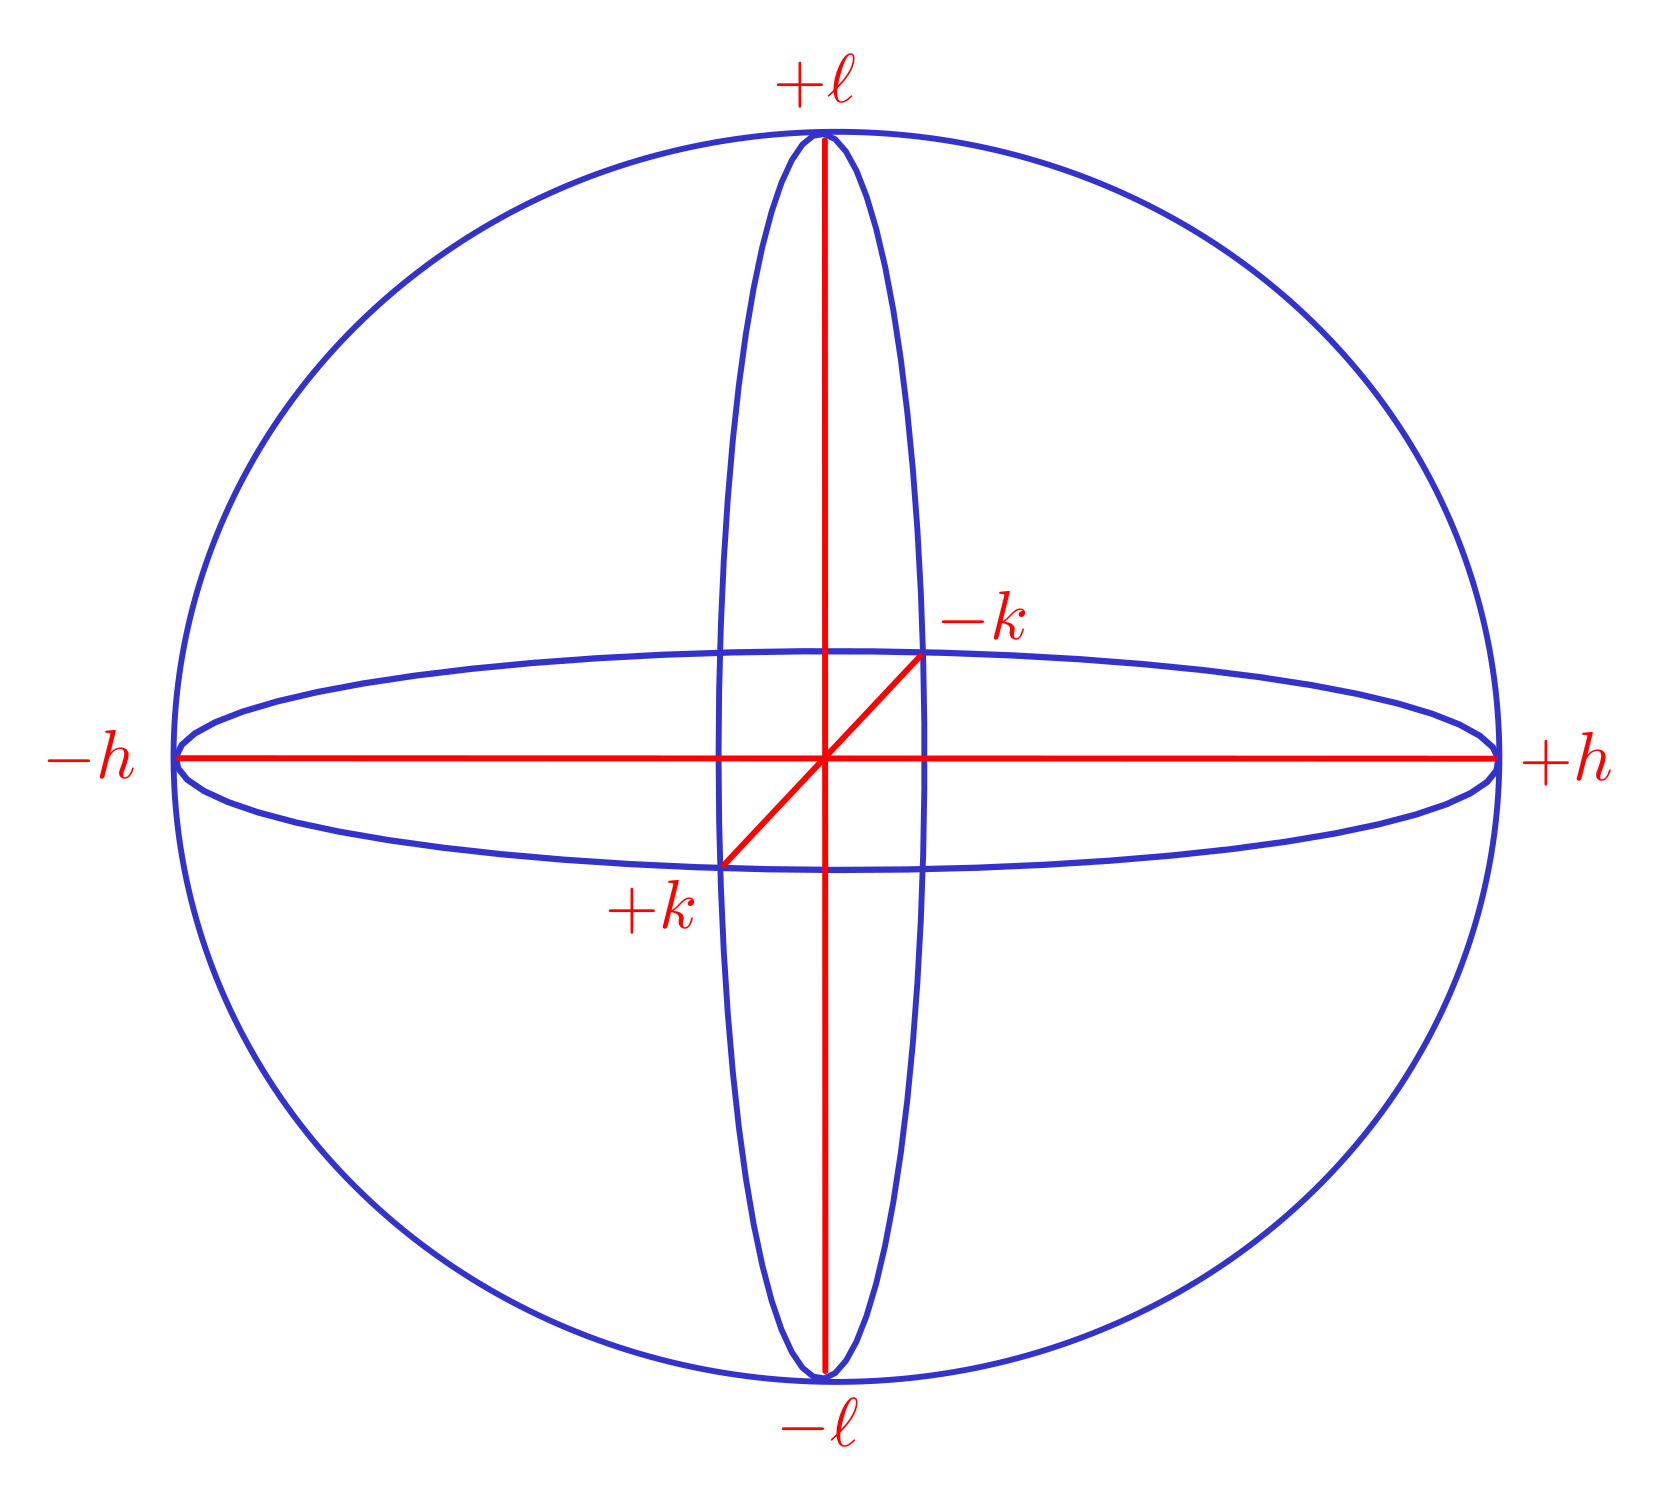
\includegraphics[scale=0.15]{full_sphere.png}
	\caption{\label{fig:full_sphere}Full sphere of data. All of $x$, $y$ and $z$ range from $-\infty$ through $0$ to $+\infty.$}
\end{figure}

A \textbf{full sphere of data} (figure~\ref{fig:full_sphere}) corresponds to%
%	
	\begin{itemize}%
%	
	    \item $h$ from $-\infty$ through $0$ to $+\infty,$
	    
	    \item $k$ from $-\infty$ through $0$ to $+\infty,$ and
	    
	    \item $\ell$ from $-\infty$ through $0$ to $+\infty.$
	    
	\end{itemize}
	
\begin{figure}
	\centering
	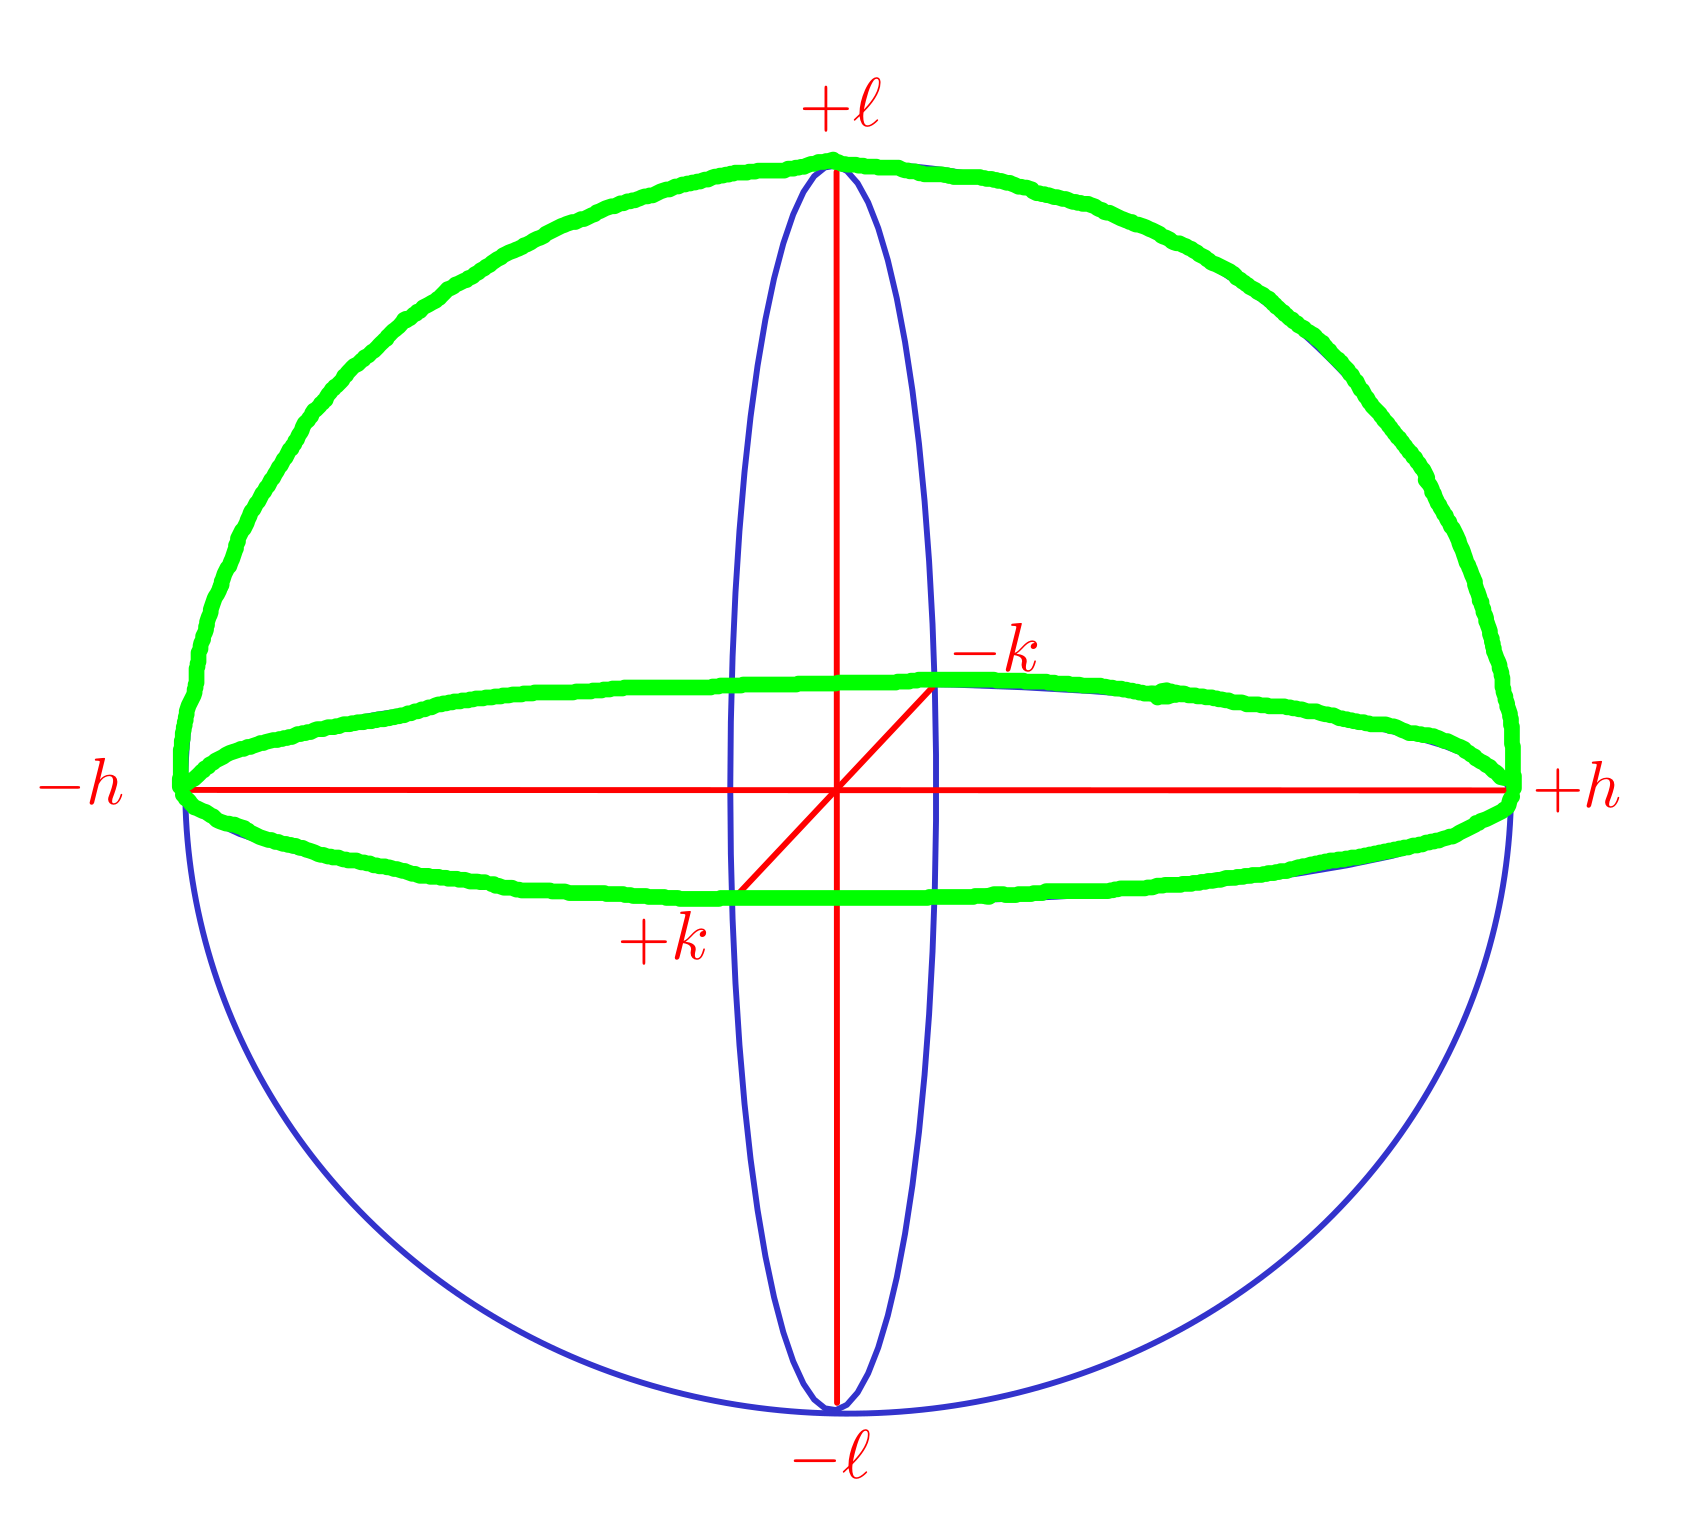
\includegraphics[scale=0.15]{hemisphere_data.png}
	\caption{\label{fig:hemisphere}A hemisphere of data corresponds to the closed region demarcated in green. The lower hemisphere is also equally valid due to Friedel's Law.}
\end{figure}
	
A \textbf{hemisphere of data} (figure~\ref{fig:hemisphere}) implies that one index among $h$, $k$ and $\ell$ will run from $0$ to $+\infty,$ and the other two indices will range from $-\infty$ through $0$ to $+\infty.$
	
The maximum \textbf{Laue symmetry} of a particular crystal system, combined with Friedel's law, tells us how much data is sufficient for a particular crystal system.

A \ul{triclinic system}, for instance, has only two possible crystallographic symmetries: $1$ and $\bar{1},$ and hence, the maximum Laue symmetry is $\bar{1}.$  This is basically a centre of inversion symmetry. Therefore, only Friedel's Law applies here, and we have to record only a hemisphere of data.

\begin{figure}
	\centering
	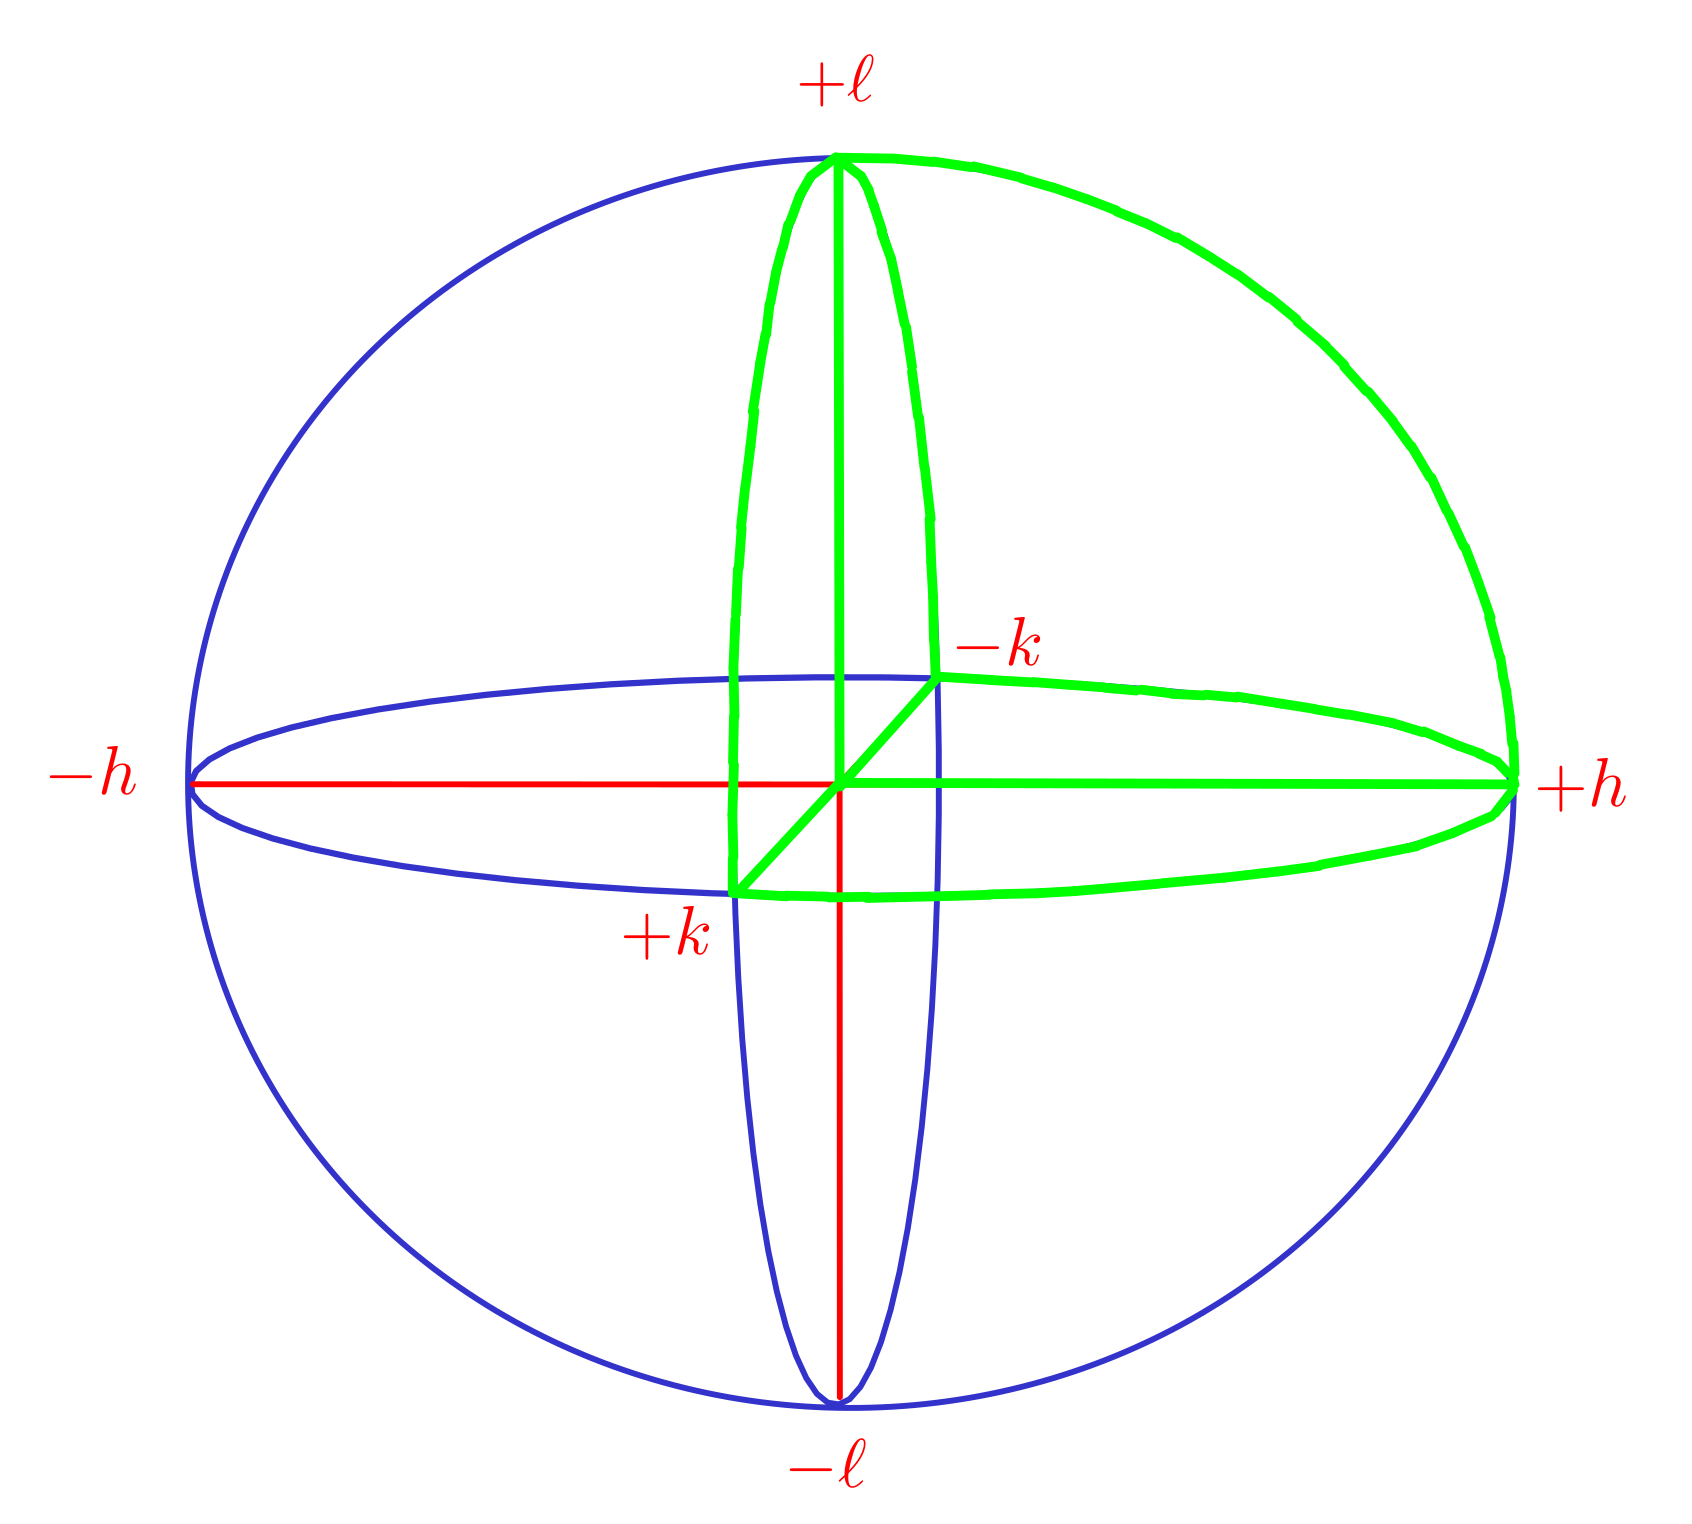
\includegraphics[scale=0.15]{one_fourth_sphere1.png}
	\caption{\label{fig:one_fourth_sphere}For a monoclinic system, only one-fourth data (the demarcated region) is sufficient.}
\end{figure}

For a \ul{monoclinic system}, the maximum Laue symmetry is $2/m,$ which is a 2-fold rotation axis, and a mirror plane $m \perp$ the rotation axis. If we consider $y$ to be the unique axis, such that $2 \parallel y$, then we have two sets of reflections:%
%	
\begin{equation}
\tikzmarknode[is]{a}{I}_{\tikzmarknode[is]{b}{h}kl}
    \equiv I_{\tikzmarknode[is]{c}{\bar{h}} \bar{k} \bar{\ell}}
    \equiv I_{\tikzmarknode[is]{d}{\bar{h}} \tikzmarknode[is]{e}{k} \bar{\ell}}
    \equiv I_{\tikzmarknode[is]{f1}{h} \tikzmarknode[is]{f}{\bar{k}} \ell}
\end{equation}
%
\begin{center}  % <--- for space of image
%
\begin{tikzpicture}[remember picture, overlay]
\draw[ ->, blue]          ([xshift=+1pt] b) |-|[distance=5mm]  (c.south) node[lbl, pos=0.5] {FL};
\draw[ ->, teal]    ([xshift=-1pt] b) |-|[distance=9mm]  (d.south) node[lbl, pos=0.6] {$2 \parallel y$};
\draw[ ->, purple]  ([xshift=+1pt] a) |-|[distance=15mm] (f.south) node[lbl, pos=0.65] {$m \perp y$};
%
\draw[ <->, blue]    (e.south) to[bend right=45, "FL" lbl=north] (f1.south);
\end{tikzpicture}
%
\vspace{10ex}        % <--- additional space for image
%
\end{center}
%	
and%
%
\begin{equation}
\tikzmarknode[is]{a}{I}_{\tikzmarknode[is]{b}{\bar{h}} k \ell}
    \equiv I_{\tikzmarknode[is]{c}{h} \bar{k} \bar{\ell}}
    \equiv I_{\tikzmarknode[is]{d}{h} \tikzmarknode[is]{e}{k} \bar{\ell}}
    \equiv I_{\tikzmarknode[is]{f1}{\bar{h}} \tikzmarknode[is]{f}{\bar{k}} \ell}
\end{equation}
%
\begin{center}  % <--- for space of image
%
\begin{tikzpicture}[remember picture, overlay]
\draw[ ->, blue]          ([xshift=+1pt] b) |-|[distance=5mm]  (c.south) node[lbl, pos=0.5] {FL};
\draw[ ->, teal]    ([xshift=-1pt] b) |-|[distance=9mm]  (d.south) node[lbl, pos=0.6] {$2 \parallel y$};
\draw[ ->, purple]  ([xshift=+1pt] a) |-|[distance=15mm] (f.south) node[lbl, pos=0.65] {$m \perp y$};
%
\draw[ <->, blue]    (e.south) to[bend right=45, "FL" lbl=north] (f1.south);
\end{tikzpicture}
%
\vspace{10ex}        % <--- additional space for image
%
\end{center}
%
where ``FL`` stands for Friedel's Law.

We only need to record one each from these two sets, and the minimum number of reflections required to be recorded is reduced to one-fourth, shown in figure~\ref{fig:one_fourth_sphere}. Thus, the range of $h,$ $k$ and $\ell$ is as follows:%
%	
	\begin{itemize}%
%	
	    \item $k \tendsto 0$ to $+\infty$ (as $y$ is the unique axis), \textit{and}
	    
	    \item $h \tendsto 0$ to $+\infty$ and $\ell \tendsto -\infty$ to $+\infty$, \textit{or}
	    
	    \item $h \tendsto -\infty$ to $+\infty$ and $\ell \tendsto 0$ to $+\infty.$
	    
	\end{itemize}

For an \ul{orthorhombic system}, the maximum Laue symmetry is $mmm \implies m \perp x,\ m \perp y,\ m \perp z.$ Thus, the following reflections are all equivalent:%
%
\begin{equation}
\tikzmarknode[is]{a}{I}_{\tikzmarknode[is]{b}{h}kl}
    \equiv I_{\tikzmarknode[is]{c}{\bar{h}} \bar{k} \bar{\ell}}
    \equiv I_{\tikzmarknode[is]{d}{\bar{h}} \tikzmarknode[is]{e}{k} \ell}
    \equiv I_{h \tikzmarknode[is]{f}{\bar{k}} \bar{\ell}}
    \equiv \tikzmarknode[is]{g}{I}_{h \bar{k} \tikzmarknode[is]{h}{\ell}}
    \equiv I_{\bar{h} k \tikzmarknode[is]{i}{\bar{\ell}}}
    \equiv \tikzmarknode[is]{j}{I}_{h k \tikzmarknode[is]{k}{\bar{\ell}}}
    \equiv I_{\bar{h} \tikzmarknode[is]{l}{\bar{k}} \ell}
\end{equation}
\begin{center}  % <--- for space of image
\begin{tikzpicture}[remember picture, overlay]
\draw[ ->, blue]          ([xshift=+1pt] b) |-|[distance=5mm]  (c.south) node[lbl, pos=0.5] {FL};
\draw[ ->, teal]    ([xshift=-1pt] b) |-|[distance=9mm]  (d.south) node[lbl, pos=0.6] {$m \perp x$};
\draw[ ->, purple]  ([xshift=+1pt] a) |-|[distance=13mm] (g.south) node[lbl, pos=0.65] {$m \perp y$};
\draw[ ->, orange]  ([xshift=-1pt] a) |-|[distance=18mm] (j.south) node[lbl, pos=0.7] {$m \perp z$};
%
\draw[ <->, blue]    (e.south) to[bend right=45, "FL" lbl=north] (f.south);
\draw[ <->, blue]    (h.south) to[bend right=45, "FL" lbl=north] (i.south);
\draw[ <->, blue]    (k.south) to[bend right=45, "FL" lbl=north] (l.south);
\end{tikzpicture}
\vspace{10ex}        % <--- additional space for image
\end{center}
%
and we need to record only one from this set. Thus, the data to be recorded decreases to one-eighth for an orthorhombic system, and we need to only record the region highlighted in figure~\ref{fig:one_eighth_sphere}.

\begin{figure}
	\centering
	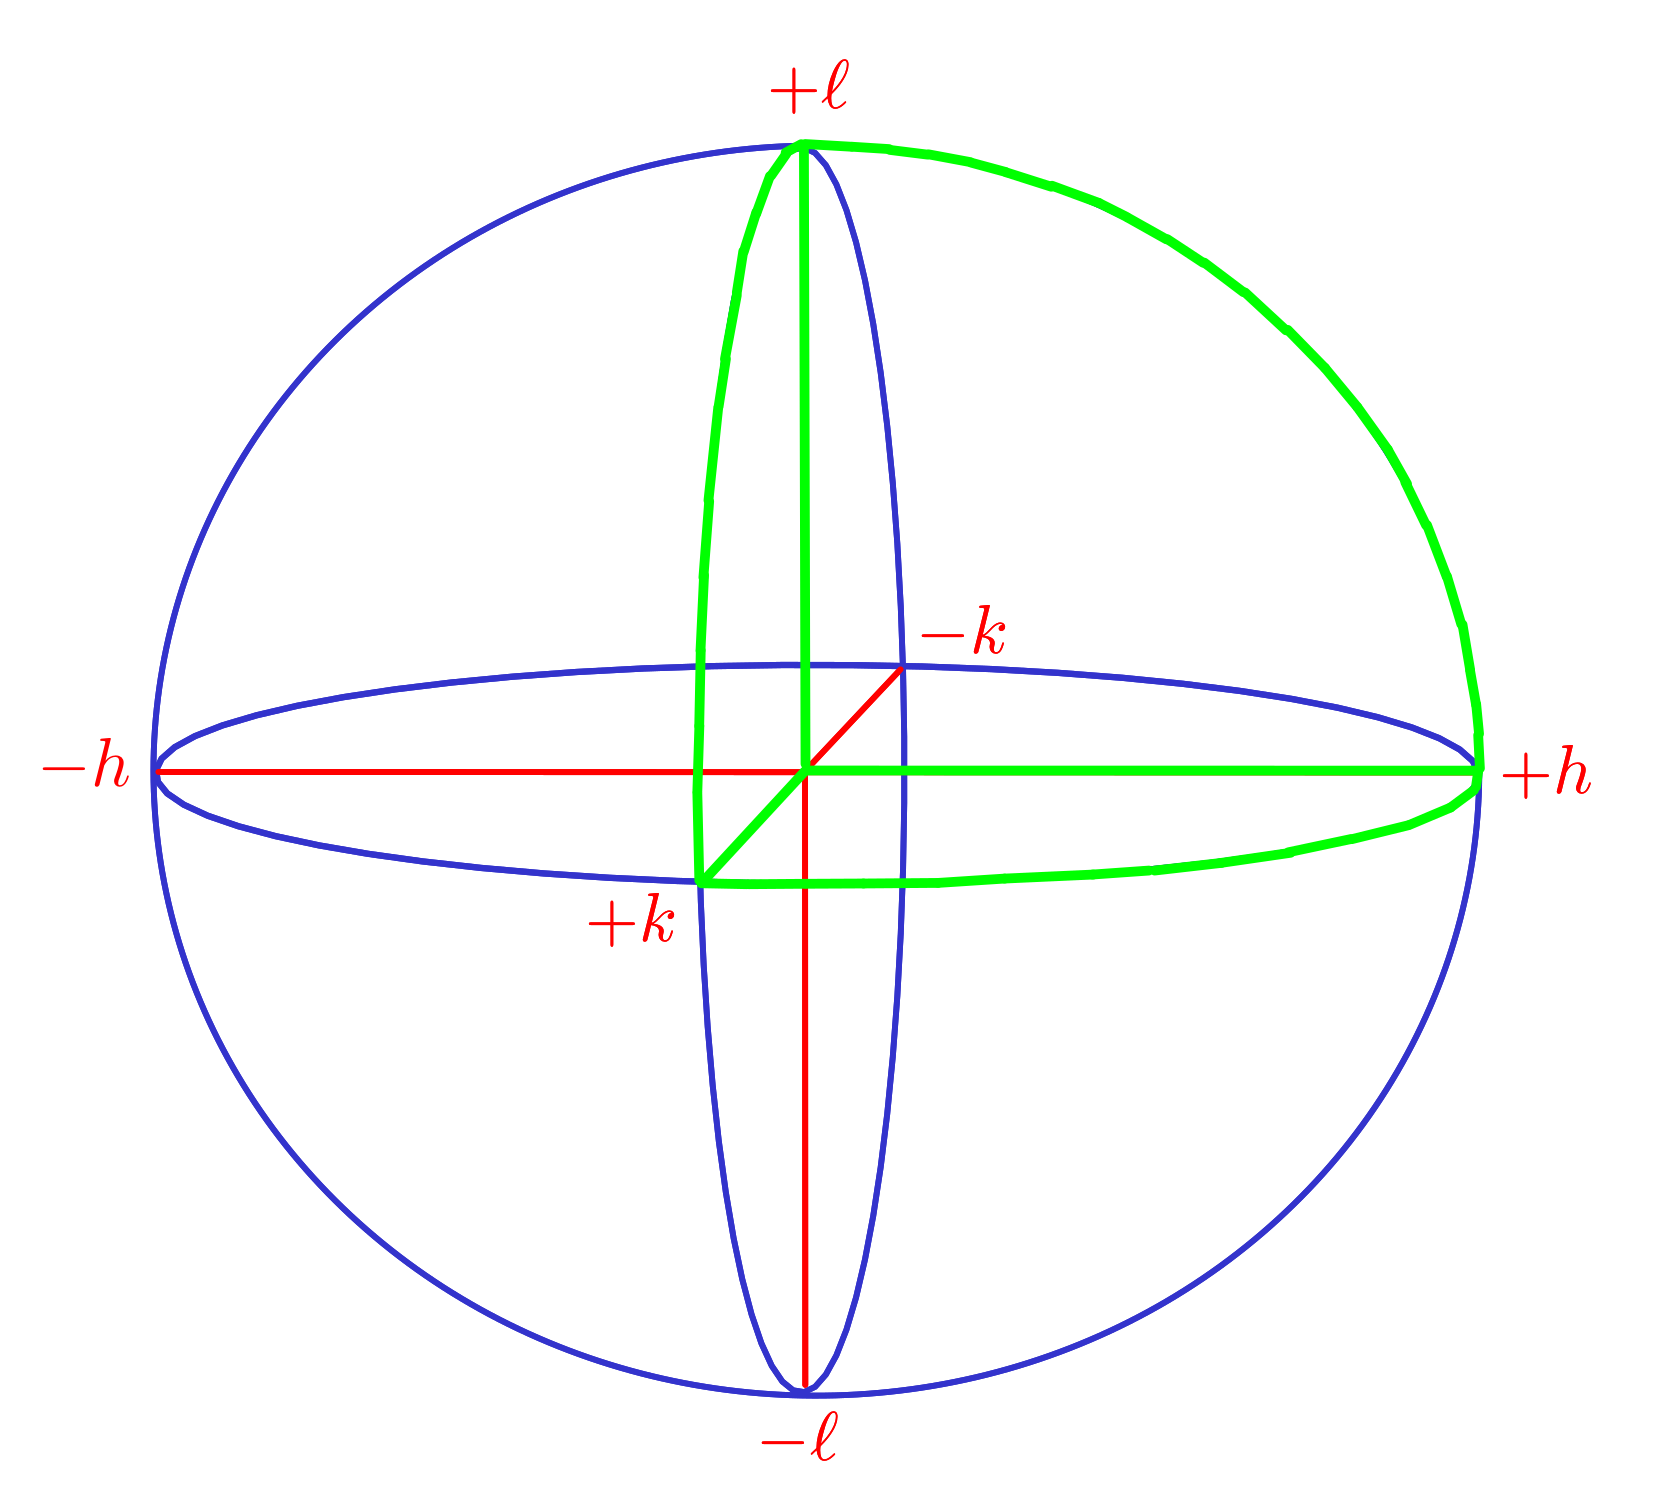
\includegraphics[scale=0.15]{one_eighth_sphere.png}
	\caption{\label{fig:one_eighth_sphere}For an orthorhombic system, only one-eighth sphere data (the region demarcated in green) is sufficient.}
\end{figure}

Understanding how much data we have to collect for different crystal systems was extremely essential even, say, 20 years back. In those days, the detector in the diffractometer used to be a point detector. Such a detector can record only one reflection at a time, and it would take quite a long time to center a reflection at the maxima and then record the intensity. 

When we mount a crystal on the diffractometer and rotate it about the $\phi$ axis, diffraction would be visible from all directions. The detector, however, being a point detector, could only measure in a particular plane. The procedure used was as follows: First, the detector would be moved to the location of a particular reflection. Next, the detector would be moved in very small steps to locate the maxima of the diffracted light. Thereafter, the crystal would be very slowly rotated about the different axes of the diffractometer to maximize the intensity once again. Thus, for recording a particular reflection, it would take 5-7 minutes. If the intensity is weak at that point, it would take at least 15 minutes to get sufficient data. So, without Friedel's Law, one would have to spend more than a week to record all reflections.

Suppose, for a tricilinic system, 10,000 reflections are possible considering all $(hk\ell)$ and $(\bar{h} \bar{k} \bar{\ell}).$ It would take around 6-8 days for this data to be collected. Thanks to Friedel's Law, we know that we have to collect only half of the data rather than the full sphere. If we know whether the crystal is monoclinic, triclinic or orthorhombic, data collection time reduces further.

Even with the advent of modern area detectors, Friedel's Law is still equally useful.
	
	\bibliographystyle{IEEEtran}
	\bibliography{bibliography}
		

\end{document}